%%%%%%%%%%%%% 5 %%%%%%%%%%%%%%%%%%%%%%%%%%%%%%%%%%%%%%%%%%%%%%%%%%%%%%%%%%%%%%%%%%%%%%%%%%%%%%%%%%%%%%%%%%%%%%%%%%%%%%%%
\chapter{Analysis of ANITAIII Flight Data}
%%%%%%%%%%%%%%%%%%%%%%%%%%%%%%%%%%%%%%%%%%%%%%%%%%%%%%%%%%%%%%%%%%%%%%%%%%%%%%%%%%%%%%%%%%%%%%%%%%%%%%%%%%%%%%%%%%%%%%%%
\section{ANITAIII Analysis Overview}%1

	\subsection{Analysis goals}
	The physics event search analysis detailed in this thesis was designed to find ``cosmic ray like'' events specifically.  The flux and energy spectrum of CRs has been well measured, and there are already published observations of cosmic rays from previous ANITA flights. The blinding requirements and associated drawbacks of doing a full blind analysis for previously unobserved impulsive signals, such as in-ice $\nu_{e}$ and $\nu_{\mu}$ interactions, can be greatly diminished by approaching the analysis in this manner.  This analysis is designed to provide the highest possible exposure to a very specific signal, that of modeled and observed CR EAS impulses.  This has the consequence of reducing sensitivity to signals that do not fit into the expectation provided by measurements and models of CR EAS radiation patterns.
	
	This search is expected to be sensitive to two separate astrophysical particle interactions described in Section \ref{sec:SignalsAndBackgrounds}.  UHECRs interacting in the atmosphere and viewed directly or as a reflection off the continental ice sheet will be detectable by design.  In addition, UHE$\nu_{\tau}$ particles transiting through the Earth will also be uncovered.  Their shower profiles are expected to be very similar~\cite{tauEMShowers}, with the primary difference being absolute polarity of the signal.  An upward traveling UHE$\nu_{\tau}$ observed below the horizon would have radiation measured directly, whereas a UHECR viewed below the horizon would be observable in a reflection.  This reflection would induce a polarity flip in the electric field oriented parallel to the surface of the earth.  Since the observed signal is dominated by geomagnetically induced radiation, which at the poles are primarily vertically aligned, the strongest E-field component would be horizontally polarized.
	
	The results of this analysis will be an accounting of the signals found using this search method and the estimated exposure the ANITA-III instrument had during its flight to this type of astrophysical event.  The polarity of the signals will also be identified, offering a measurement of the UHE$\nu_{\tau}$ flux.  Finally, a background estimate that is novel to the ANITA experiment will be introduced and applied to the data.
	
	\subsection{Analysis outline}
	Analysis of the data recorded by the ANITAIII flight instrument requires a significant computational effort to extract a meaningful physics result.  The digital values recorded by the instruments on-board the payload, when properly calibrated and used in conjunction with one another, can establish whether any electromagnetic signals were traversing the payload at the time that the trigger system latched the digitizers.  The combination of geometric antenna offsets and their corresponding timing delays allows the discrimination of signal versus noise, as well as precision reconstruction of any incident signal.  Using a variety of mathematical methods and an understanding of the expected signal, the nearly 85 million waveforms captured during the flight can be pared down to a handful of likely CR candidates, which can then be examined in greater detail.  This chapter details the calculated values, their motivations, and the methods used to conduct the cosmic ray search.
	
	A diagram that depicts the order in which analysis steps are taken, as well as their relavant software packages and intermediate files, is shown in Figure \ref{fig:AnalysisDiagram}. 
	
\begin{figure}
	\centering
	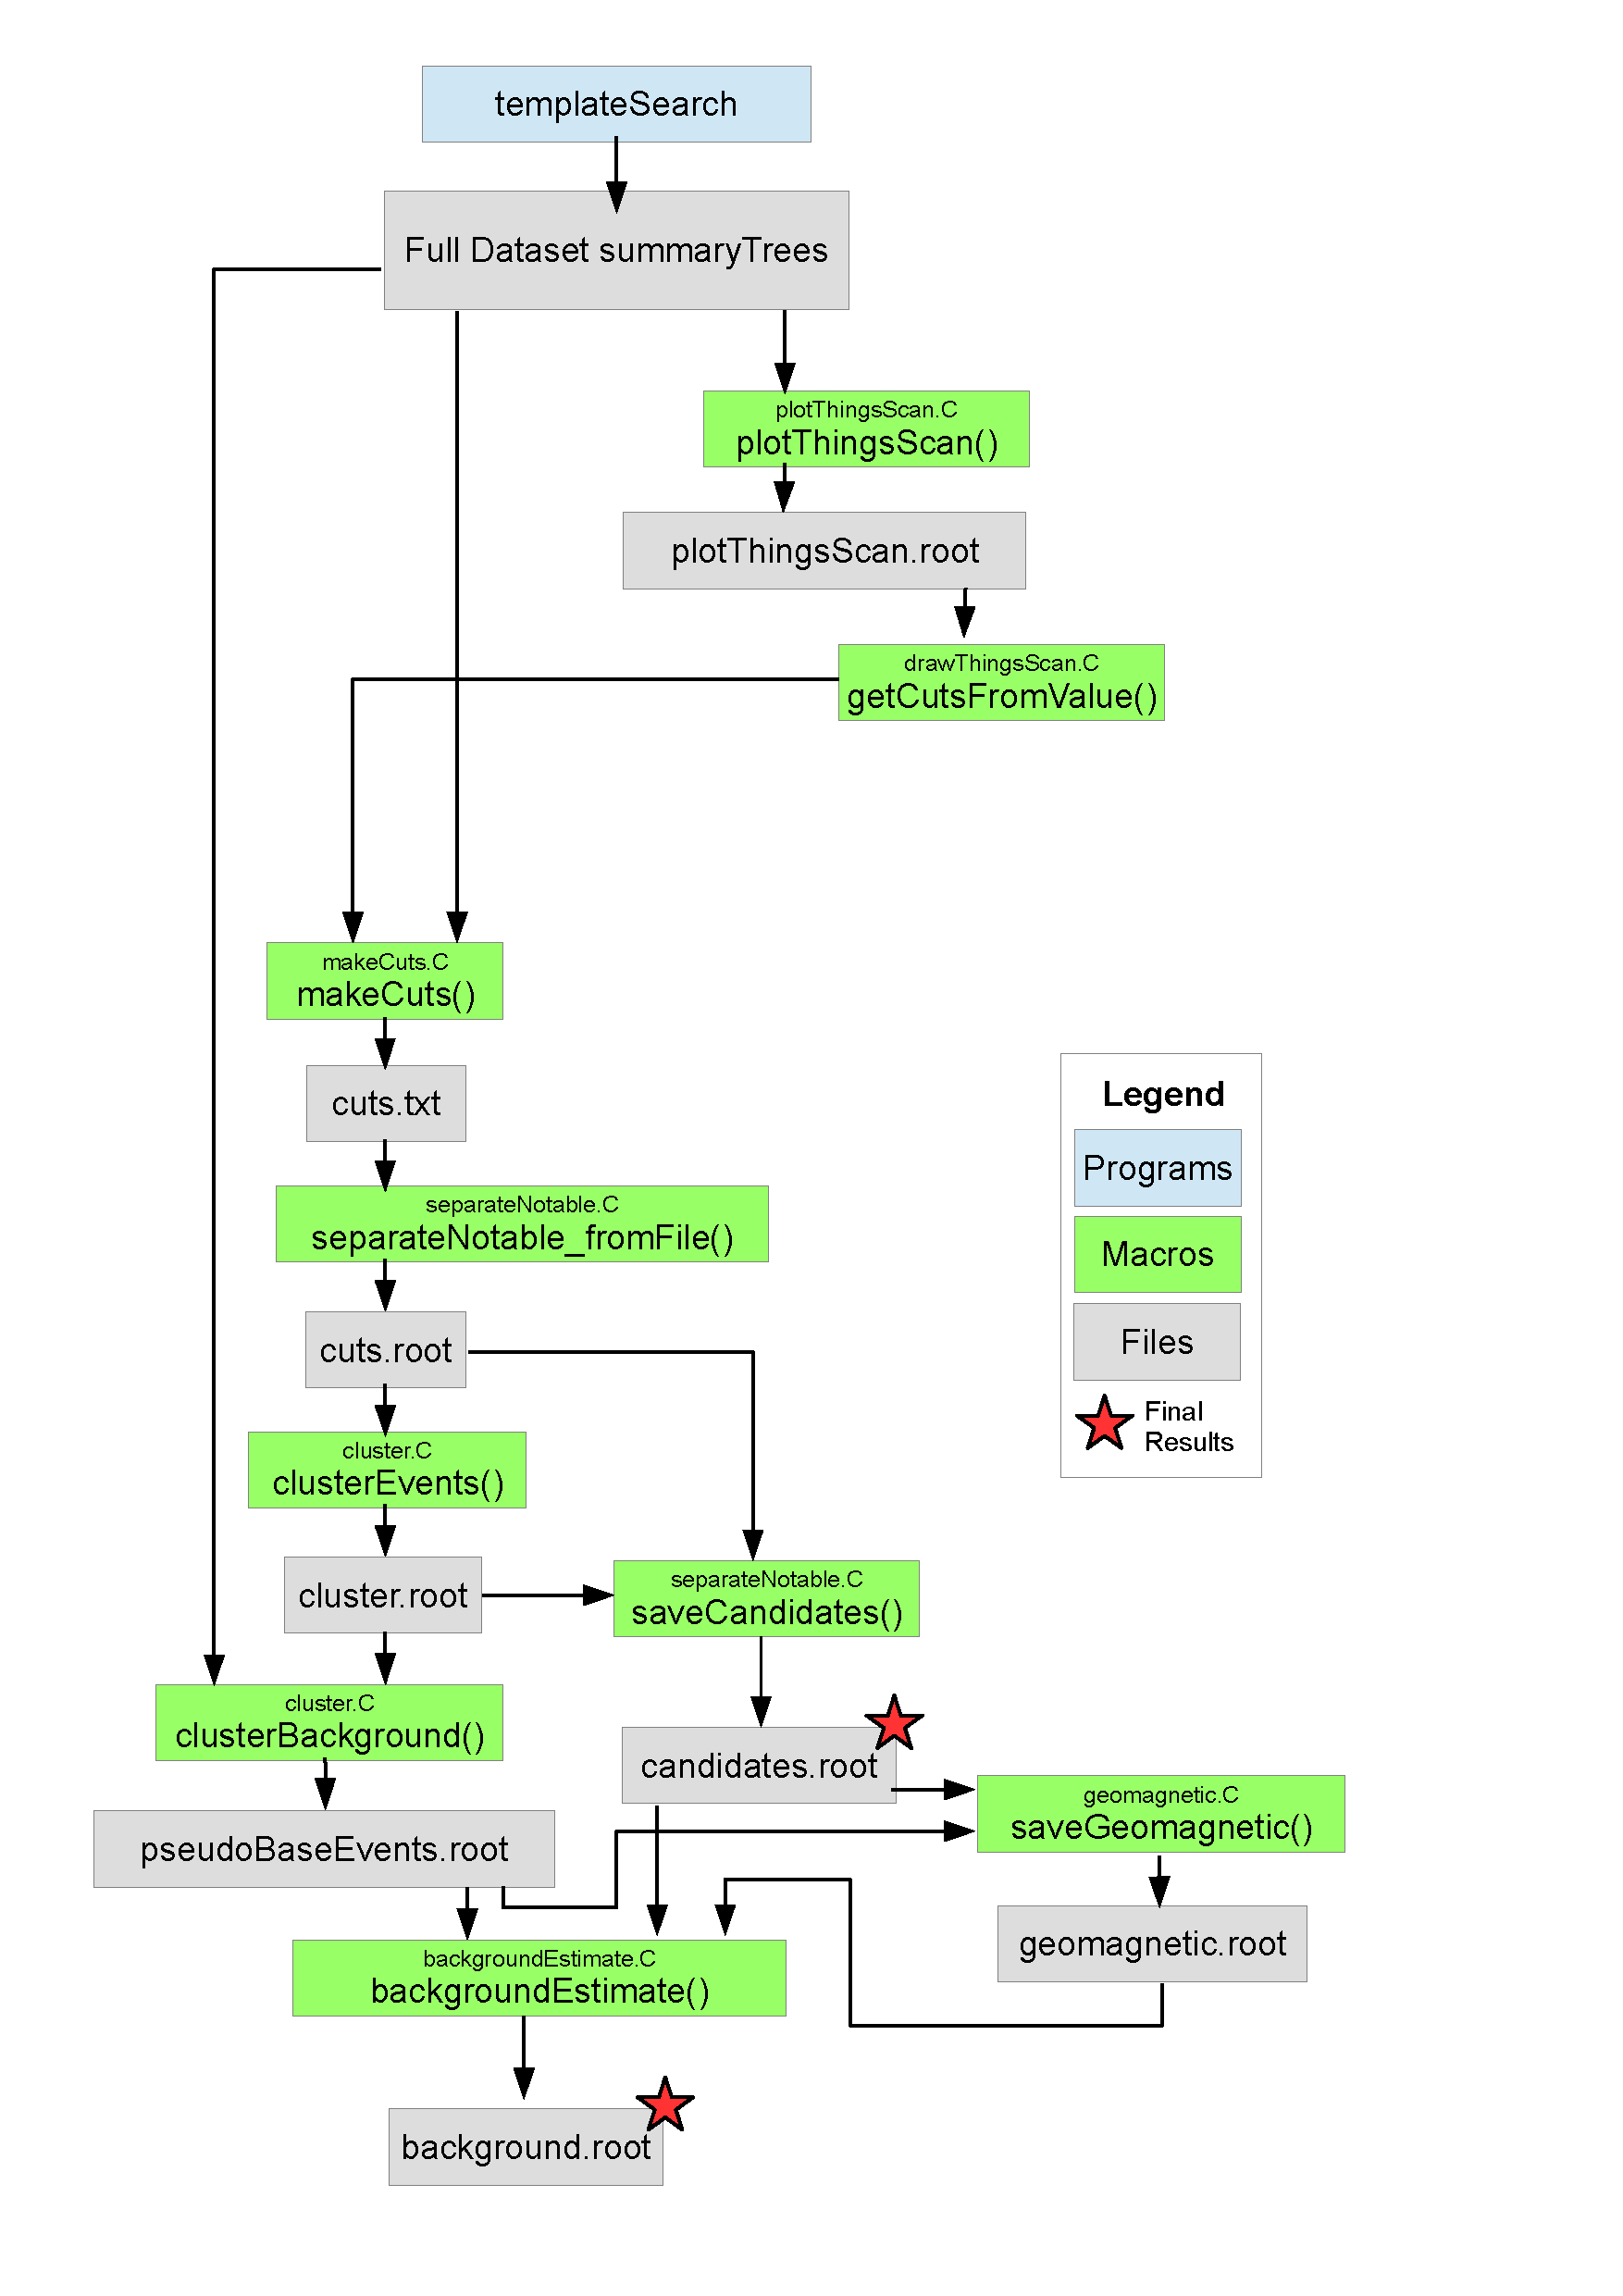
\includegraphics[height=0.8\textheight]{figures/AnalysisDiagram}
	\caption{A diagram depicting the order in which analysis steps are taken, the intermediate storage files saved to disk, and the function names and ROOT macros where the bulk of the code is located.  The calculations and algorithms contained within this code-base is described in detail throughout this chapter.  The storage locations of final results are noted with red stars.}
	\label{fig:AnalysisDiagram}
\end{figure}	
		
%	The data recorded by the ANITAIII flight instrument requires a significant analysis effort to extract a meaningful physics result.  Using the raw digital values recorded from each channel, we can establish the analog electromagnetic environment surrounding the payload during brief moments the trigger system determined a physics event may be occurring.  From this, we can use an  understanding of the physical geometry of the antennas mounted on the payload, including their orientation and electrical responses, to determine the cause of any incident wave patterns read out by the digitizers.  Once these wave patterns are identified and classified, they can be sorted into signal and noise, background thermal or anthropogenic, via a series of procedural cuts.  This section details the process and results of this analysis.
	

\section{Software Package Overview}%2
	The analysis was done with a variety of software packages created by the ANITA collaboration.  The relevant packages used for the analysis described in this thesis are described in the following section.  They range from tools for interfacing with raw data written to disk, to ANITA specific calibration and interferometric mapping, to this-thesis specific packages for template correlation, clustering, and background estimation.  The packages are described in order of dependency, with most independent packages listed first.
	
	The cosmic ray search was done primarily in C++ using libraries from the ROOT Data Analysis Framework~\cite{ROOT}.  ROOT, developed at CERN, provides a variety of data storage objects and plotting functions optimized for physics experiments.

	\subsection{ROOT FFTW interface: libRootFftwWrapper}
		Fourier transforms were done using the the Fastest Fourier Transform in the West (FFTW) package.  This package is not designed to be used with the ROOT objects that the remainder of the packages are based around, and so an interface library, named libRootFftwWrapper is used~\cite{libRootFftwWrapper}.  This package not only provides an interface however, it also includes a large number of ANITA related numerical recipes.

	\subsection{Event Reader Software: eventReaderRoot}
		The data taken by the ANITAIII instrument is written in a compressed C++ binary class format to disk.  This data format requires minimal computational load and very fast write speeds, with minimal storage space overhead.  This data format requires a standardized class structure that is stored in the eventReaderRoot code library~\cite{eventReaderRoot} in order to accurately read and extract any values.  The raw data taken in flight is converted to ROOT objects, which increases data read speed and enforces data quality, with the tradeoff of slightly increased storage space and a one time computationally complex conversion.  The eventReaderRoot library also stores information about each flight, such as the number of antennas and their mapping to RF channel, as well as tools for applying the calibration constants to waveforms.

	\subsection{Coordinated Analysis Framework: AnitaAnalysisFramework}
		In order to facilitate active collaboration between multiple analyzers, much of the analysis software was consolidated into a library named the Anita Analysis Framework~\cite{anitaAnalysisFramework}.  It provides a standardized set of C++ classes for storing and calibrating digitized LABRADOR waveforms in memory, implementing filtering algorithms, implementing agreed-upon common analysis tools, and a shared output format.
		
		This framework, most importantly, provides a C++ summary class with agreed upon reduced quantity values of interest.  This object, named the AnitaEventSummary, is created for each event taken during the flight, and is designed to be filled by any analysis routine with all values required to do a full physics analysis of the flight data.  This prevents computationally burdensome calculations used in calibration and interferometry from being repeated multiple times.
				
				%crab
	\subsection{University of Chicago Event Analyzer: UCorrelator}
		The data taken by the ANITA instrument requires processing to be useful in a physics analysis, and many of the computational techniques can be shared across multiple analyses.  For this analysis, I have used, and collaborated, to the UCorrelator software package developed primarily by Cosmin Deaconu at the University of Chicago~\cite{UCorrelator}.  With the addition of my own bug-testing and feature expansion, this package has been used to do the base-level numerical computations for this analysis.
		
		
	\subsection{Event Display: anitaMagicDisplay}
		The anitaMagicDisplay package \cite{anitaMagicDisplay} allows a user to quickly and easily display many of the most relevant raw and reduced data values for any event in the flight.  The package provides a Graphical User Interface (GUI) that can simultaneously display waveforms captured from the entire instrument sorted in various ways.  It also includes dynamically selectable filtering strategies, maps and summaries of multiple interferometric reconstruction techniques, and payload orientation information.  
		
	\subsection{Miscellaneous utility functions: anitaEventCorrelator}
		A separate library that includes some additional important functionality is anitaEventCorrelator~\cite{anitaEventCorrelator}.  The most important class in this code is UsefulAdu5Pat, which takes raw GPS sensor information, as well as Earth geometry and Antarctic topographical information, and provides a method for mapping spherical payload coordinates to a point on the continent, and vice-versa.
		
		
	\subsection{Thesis analysis specific: benCode}
		The eclectic accumulation of code used in this analysis is stored in a variety of libraries, macros, and compiled programs collectively named benCode~\cite{benCode}.  Though there are many offshoot routines for debugging and the determination of specific values of interest, the main path for the analysis is summarized in Figure \ref{fig:AnalysisDiagram}.

	
	
	
\section{Dataset and Blinding Procedure}%3
	
	\subsection{Dataset for analysis}
		The ANITAIII instrument was put into flight configuration on December 9th 2014, which marks the beginning of the run numbering.  However, due to non-optimal launch conditions, the payload was not launched for another week.  During this time, the system remained on, taking data at a reduced rate for last minute data validation and bug fixes.  The successful launch on December 17th 2014 at 19:23 UTC is shown in Figure \ref{fig:AnitaLaunchAltitude}.  The pre-amplifiers were turned on midway through the ascent in order to protect them from the high powered anthropogenic noise at the launch facility. Run 130 is the first run at altitude with all systems operating in final flight configuration.  Run 439 was the final run recorded to disk before the instrument was powered down for descent.  The final event was taken on January 9th 2015 at 05:52 UTC.
			
\begin{figure}
	\centering
	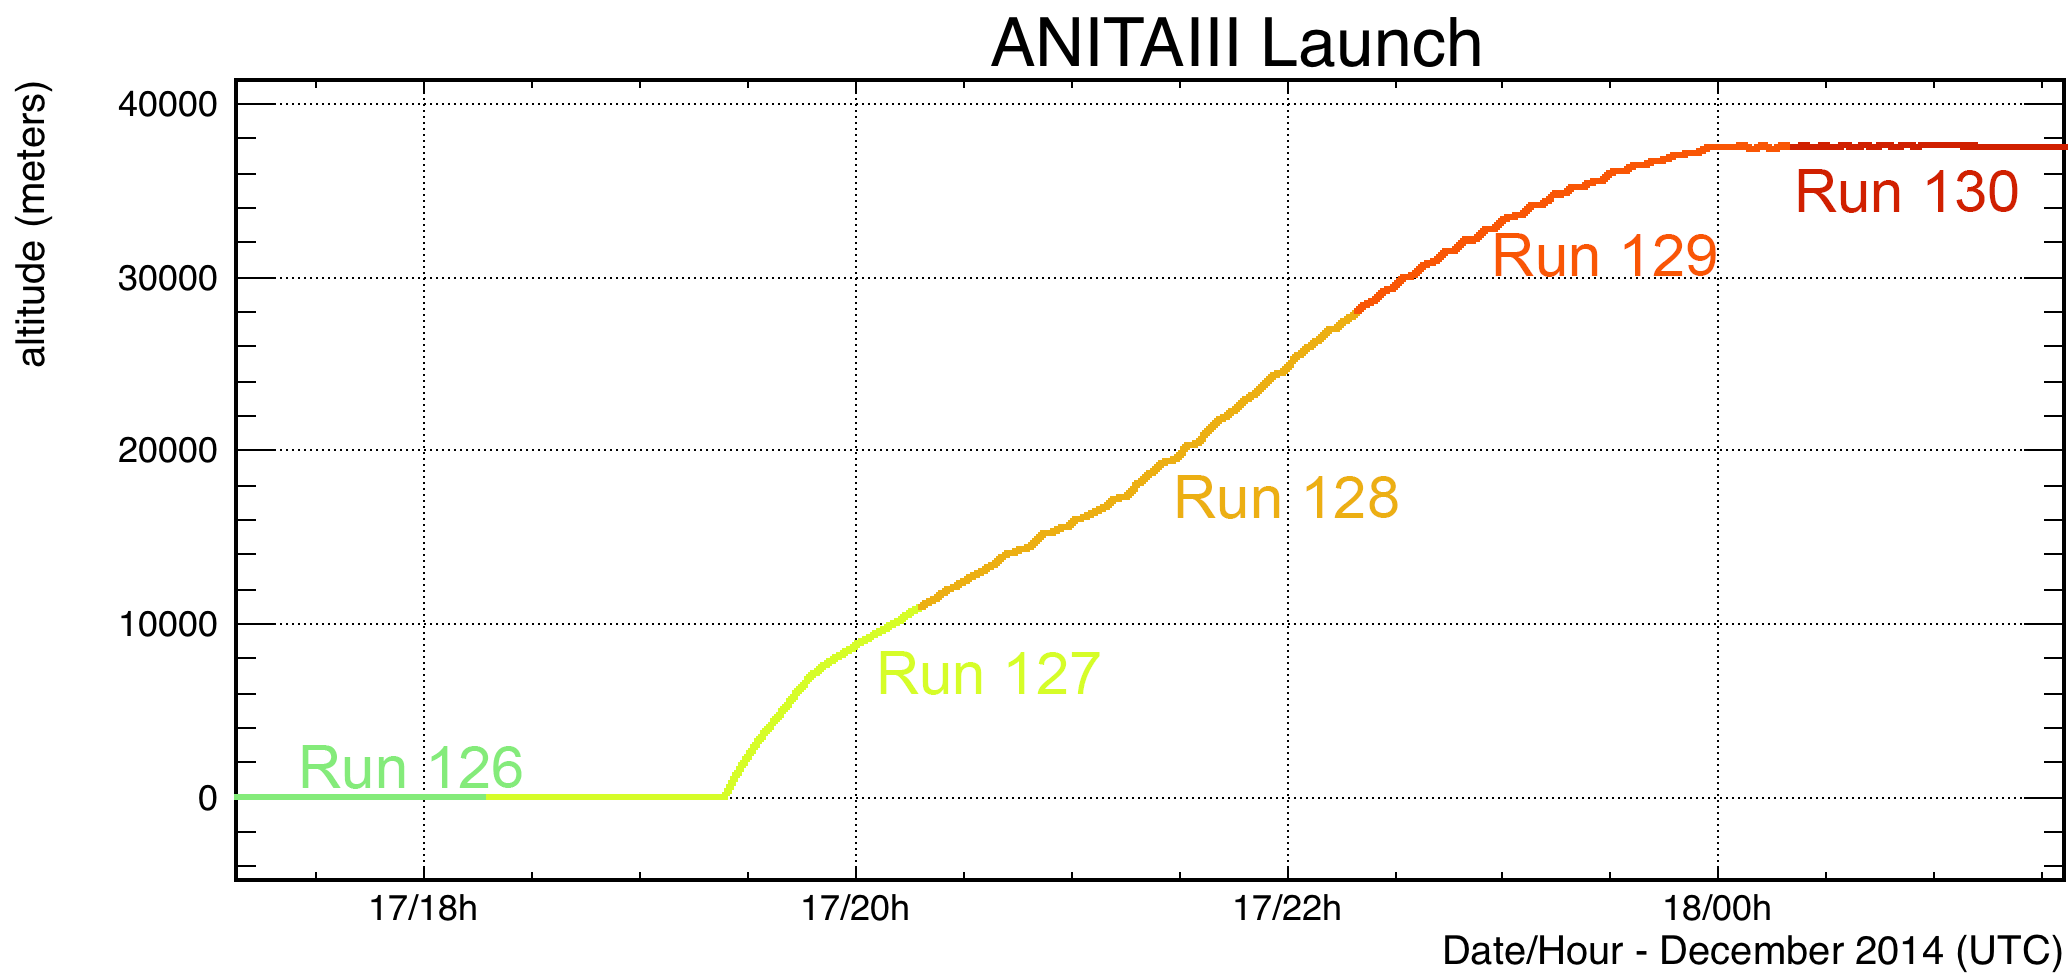
\includegraphics[width=\textwidth]{figures/LaunchAltitude}
	\caption{Altitude data captured by the on board GPS on launch day.  Colors refer to the run number of that data.  Run 130 is the first run where the instrument was in full data-taking configuration and at float altitude.}
	\label{fig:AnitaLaunchAltitude}
\end{figure}	

		During the 22 days and 10 hours of active data collection at altitude, between run 130 and run 439, ANITAIII captured 78,630,542 events.  Runs 257 through 263 contain no data due to a bug in the Prioritizer daemon causing the Ramdisk to fill, and preventing the acquisition software from recording events.  This outage occurred on Christmas day, and resulted in an 11 hour data blackout, from December 25th at 17:13 to December 26th at 04:28.
		
		For the cosmic ray analysis, only events that fired the horizontally polarized L3 trigger are considered. The geomagnetic radiation that is predicted to dominate the electromagnetic emission of an EAS is expected to be mostly horizontally polzarised. 41,566,966 events fall into this dataset.  360,055 events fired both the horizontal and vertical L3 trigger, however they are not treated in any unique manner.
		
		Additionally, the payload initialized a digitization twice per second regardless of the RF trigger, once initiated by the GPS second and once initiated by the CPU.  There were 3,551,509 of these ``minimum bias'' events recorded during the flight.  These events are also processed and used to determine the background noise environment during the flight and set cuts on thermal background.
		
	
	\subsection{Philosophical reasoning for blinding and past methods}
		Much discussion took place within the collaboration in order to prevent unwanted analyzer bias from being a significant effect of any analysis result.  Unconscious bias is an inherently human trait, the cold unfeeling rules of nature do not bend to the whims of our emotions or desires.  However, by allowing analyzers to pick and choose methods and procedures and cuts, it is possible that a result may unwittingly reflect those same desires and emotions.  For example, an ambitious physicist, who desires to further his career, may see the opportunity to do so through an exciting and controversial result that makes other scientists take note of his work.  On the other extreme, an exhausted physicist, who does not want to defend a controversial result, could ``play it safe'' and tune his analysis to find a result in agreement with other experiments.  Both these biases are undesirable, but both could be subtly effecting results though no fault of either scientist.
		
		The solution to this problem is to introduce a method in which the result is entirely outside of the experimenters control until all analysis procedures are complete.  In previous ANITA analyses, this was accomplished by ``hiding'' 90\% of the signal data, only allowing analyzers to use a 10\% fraction of the full set to tune their cuts.  Once the cuts were set to meet a desired background rejection fraction, the reminder of the events that did \textit{not} meet the cut requirements would be revealed.  A statistical method, known as the ABCD method, could be used to estimate the number of background events within the signal box from purely random statistical fluctuations.  Any number of events in excess of this background estimate would then be considered signal.  This method had several drawbacks. First, an inability to determine signal from background on an event by event basis leaves a possibility that the most interesting events are background.  Additionally, it allows anthropogenic background to escape observation within the 10\% data set, requiring it to be removed manually by hand later, re-introducing bias.
		
	\subsection{ANITAIII CR blinding technique}
		For the ANITAIII CR search, it was decided that a 10\% - 90\% blinding requirement was unnecessary.  The energy spectrum and flux density of CRs are measured well up to the UHE range and the estimated number of observable events for the flight is much larger than one.  Additionally, both ANITAI and radio extension projects at terrestrial cosmic ray observatories have measured the radio EAS signature of a CR interaction with the atmosphere.  The ANITAIII results have also been subject to a fully blind analysis previously in a neutrino search that reported 4 transient events matching signal.  For this reason, a novel and more lax blinding procedure was agreed to for this search.

		The signal of greatest interest in this analysis is a regenerated tau neutrino transiting through the earth and hadronically decaying in the atmosphere.  Though the primary particle is different from a CR EAS, the shower will evolve in a similar fashion and produce a similar radio pulse.  The defining characteristic of this signal is a polarity with the same sign as a direct EAS shower observation, but with an incidence angle below the horizon (beyond misreconstruction uncertainty).  To prevent any bias in this signal channel, the polarity of all events has been randomly inverted.  This will create a random distribution of polarities, and prevent an analyzer from determining whether any particular event is of interest.
		
		Additionally, only signals that triggered the horizontally polarized L2 trigger are analyzed to preserve the integrity of the neutrino search.  Observations of CR EAS signals are expected to be primarily horizontally polarized, while in-ice neutrino interactions are expected to have primarily vertically polarized observed signals.  This also helps to reduced the computational workload, as each polarization trigger accounted for approximately half of the overall events.
		
			
		
\section{Digital filtering}%4
	The stored digital waveforms can be improved by the removal of well understood background signals.  Anthropogenic digital communications often take the form of circularly polarized constant wave (CW) sources, and are presently superimposed in much of the data.  Their sources include both manned and unmanned bases distributed throughout the continent, as well as orbiting satellites visible above the horizon.  These CW signals have a significant effect on both the trigger circuit and the post-flight analysis of digitized data. A spectrogram of a period of the flight can be seen in Figure \ref{fig:spectrogram}, with the CW peaks from satellite noise clearly visible at 220MHz and 380MHz.

\begin{figure}
	\centering
	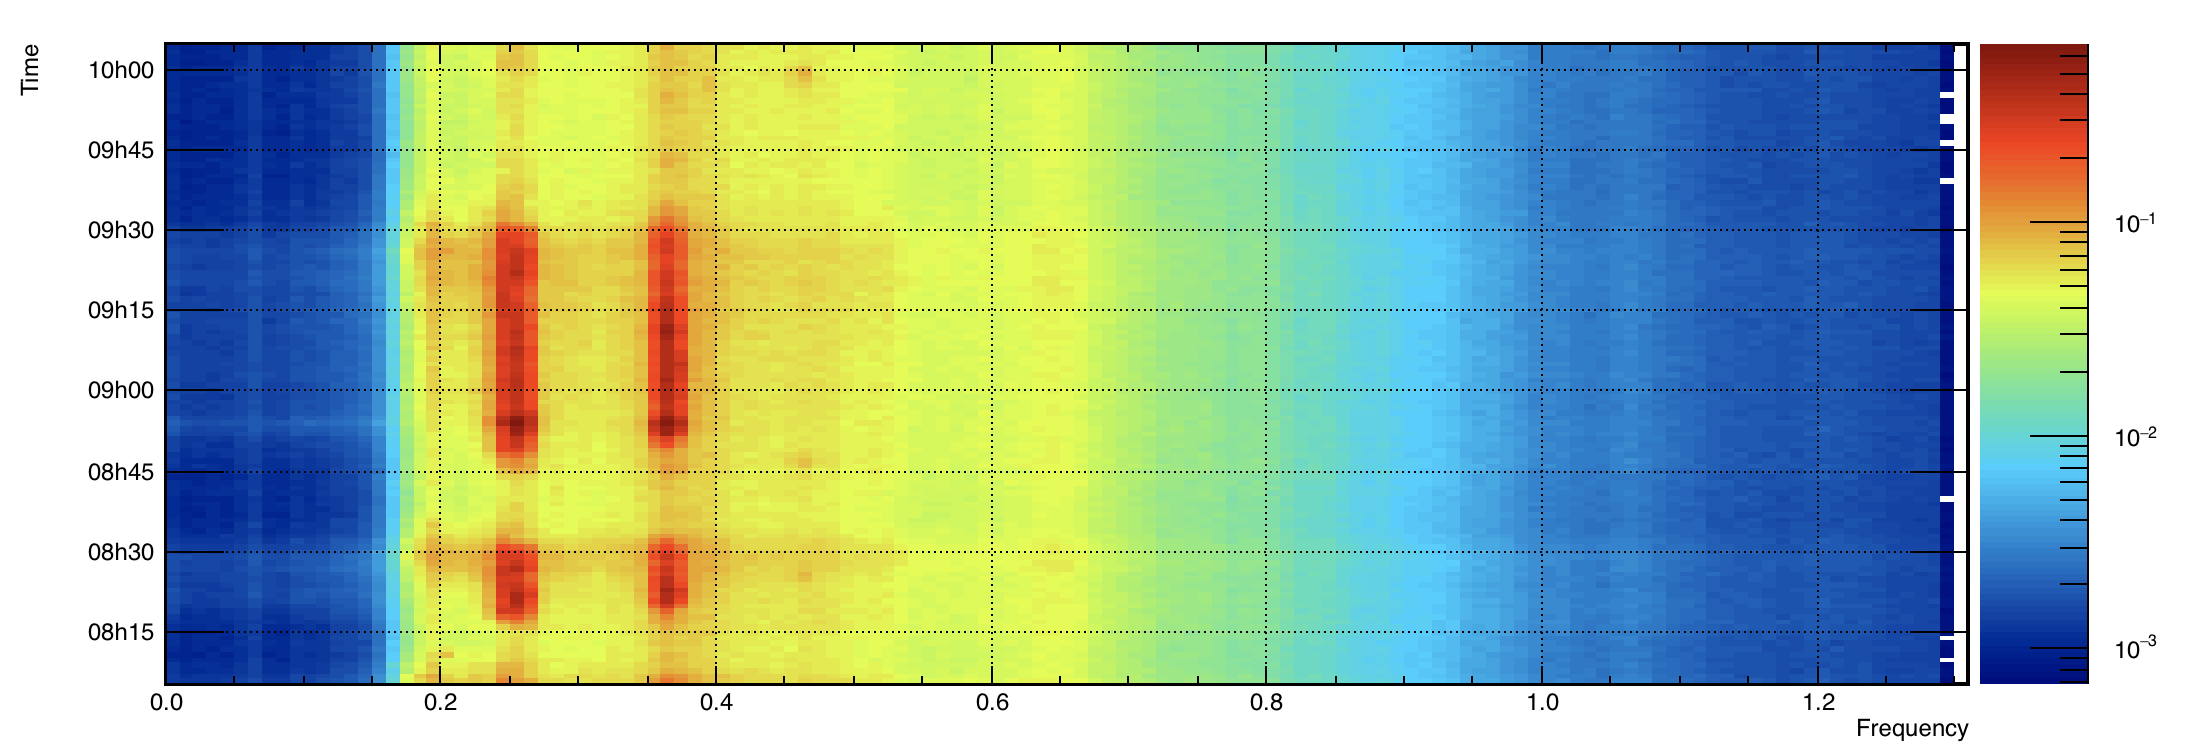
\includegraphics[width=\textwidth]{figures/spectrogram}
	\caption{A spectrogram of the measured RF signal from a single antenna pointed north during the beginning of run 371.  The Z-axis is linear power.  The red regions at 220MHz and 380MHz are frequency bands with high power due to orbiting satellites.} 
	\label{fig:spectrogram}
\end{figure}

	The effect these CW signals have on the trigger is twofold.  Firstly, they compress the tunnel diode by increasing the total power of the input signal, pushing the diode response out of its square-law range.  Additionally, CW sources force an increase in the threshold voltage used on the comparator circuit used to trigger on the signals in order to maintain an acceptable global trigger rate.  In many cases, the amount of power from CW sources forces mulitple phi sectors to self-mask, as no DAC threshold setting can appropriately limit the L2 trigger rates from a specific phi sector.  These negative effects cause a decrease in the sensitivity of the instrument to physics events with low signal power, and decrease the overall instrumented volume.  For the ANITAIV flight, a programmable analog notch filter board was flown to eliminate these effects, designed using the known CW frequencies observed in the ANITAIII flight.

	
	Despite these two effects, impulsive candidate signals can still be measured while superimposed on the CW source.  In these cases, the CW causes the interferometric image to be ``pulled'' towards the source of the signal while also presenting false peaks in the image.  To remediate the effects of these signals on the pointing and post-flight analysis, we can apply a digital filter that removes specific frequency bands.
	
	
	\subsection{Sine Subtraction Filtering}
		The filtering technique used in this analysis has been dubbed sine-wave subtraction.  Digital Finite Impulse Response (FIR) filters introduce dispersion, which will negatively effect the reconstruction accuracy and final SNR of any incident physics signal.  To alleviate this, a method was developed which involves procedurally fitting the phase, amplitude, and frequency of a sine wave to each waveform, then subtracting that sine wave from the signal.  This is repeated iteratively until the resulting subtracted wave does not have a large fractional power decrease.  This acts to remove single frequency bands from each channel without adding a significant amount of dispersion, nor diminishing physics signal or thermal noise power.  The drawback of this method is that it requires multiple fits per waveform, which is computationally expensive.  The computations for this filtering strategy takes approximately half of the total computation time.  The framework and coding of the SineSubtract algorithm was done by Cosmin Deaconu.  

	The sine subtraction works by iteratively fitting a sine wave to each captured waveform individually, minimizing on the amplitude, phase, and frequency.   To aid in computational efficiency, the range of frequencies and amplitudes that the fit could minimize over were adaptively altered based on a previously generated full flight frequency spectrogram.  This adaptive component has a configurable ``exponent'' variable that controls how strictly   This best-fit function is then subtracted from the waveform, yielding data with a single frequency component removed.  This process is repeated until the ratio of the power subtracted from the waveform over the total power in the original waveform is below some configurable threshold a specified sequential number of times.  For this analysis, a ratio of 0.1 was used, and 3 failed iterations were allowed.  The key used to generate this filter in the AnitaAnalysisFramework is ``sinsub\_10\_3\_ad\_2''.  
	
	An example of the effect that the filtering has on the interferometric map of a calibration pulser event can be seen in Figure \ref{fig:SineSubtractMaps}.  An example of the sine fit and removal over five iterations for a single waveform of the same event can be seen in \ref{fig:SineSubtractExample} 
	
\begin{figure}
	\centering
	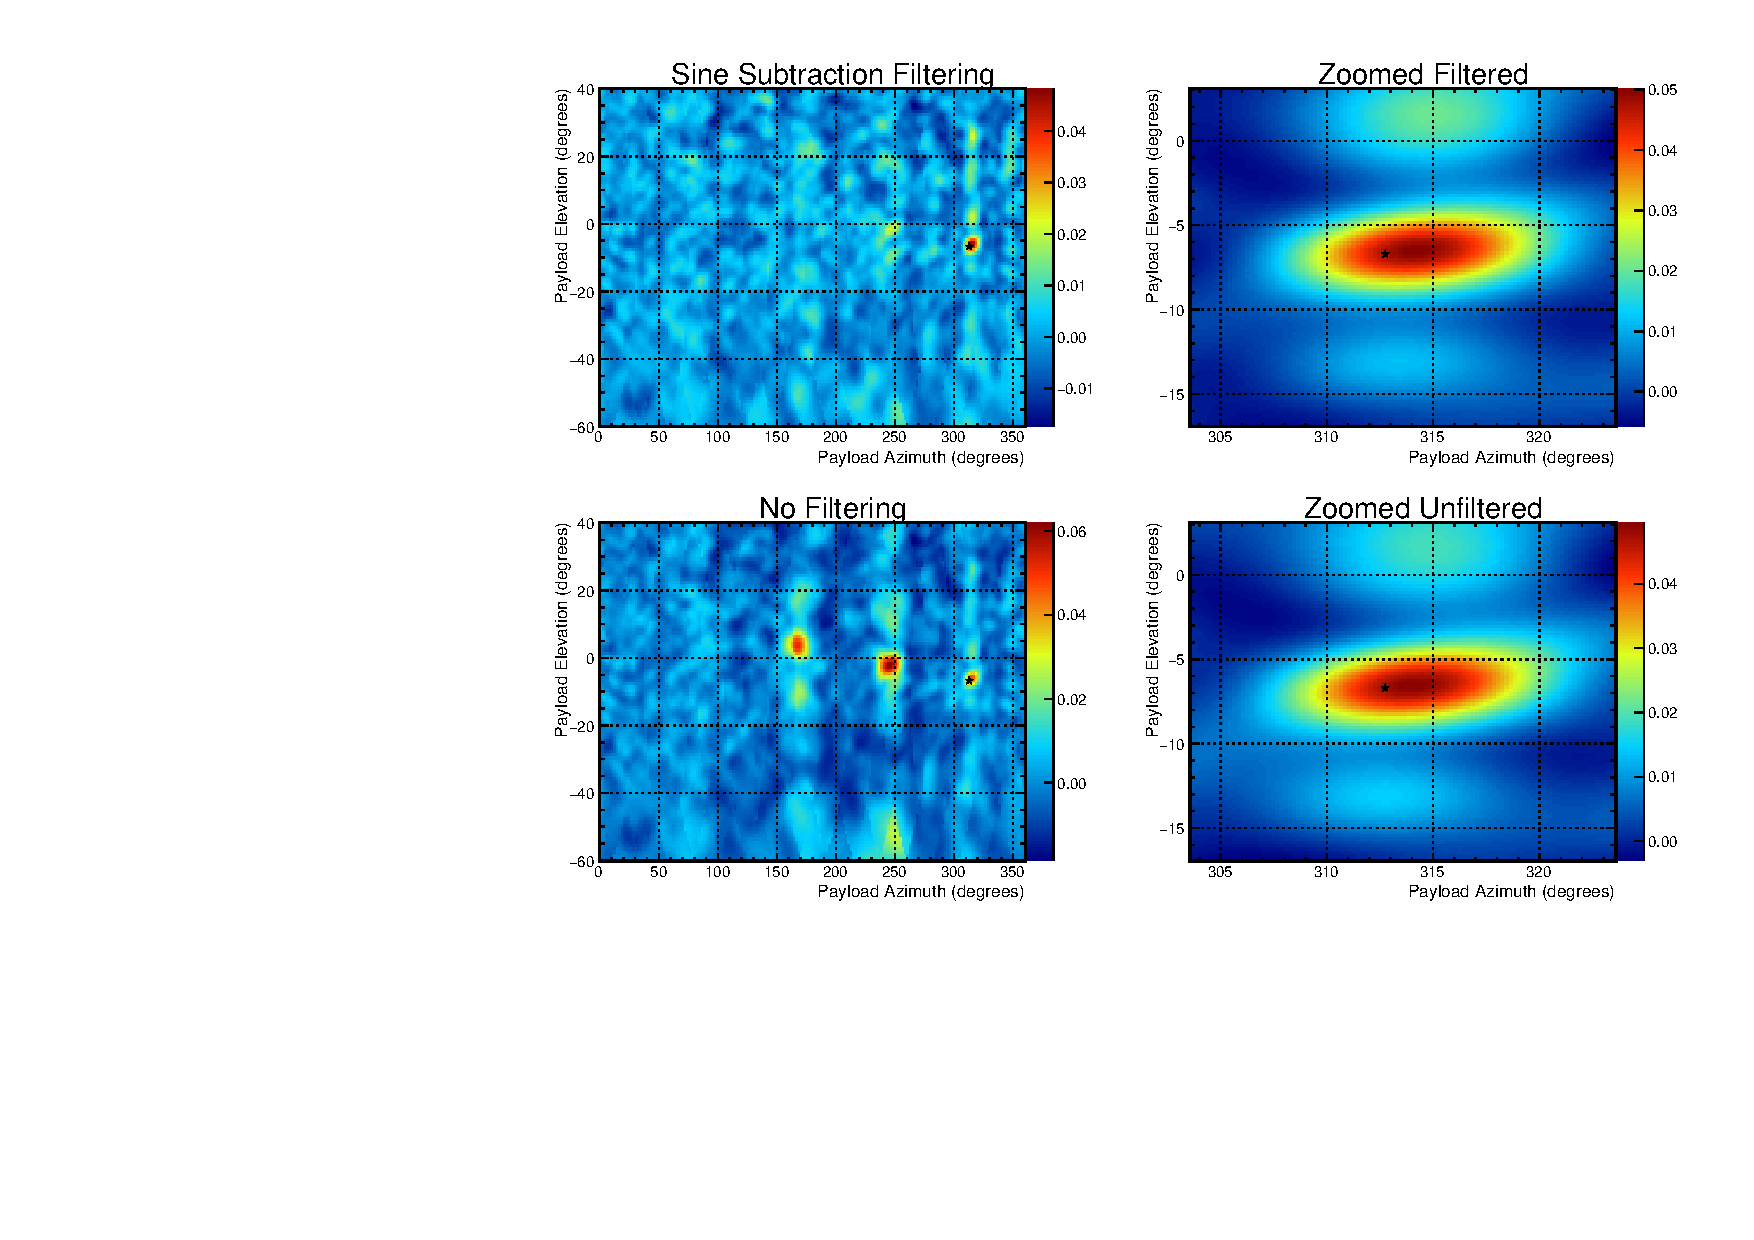
\includegraphics[height=0.5\textheight]{figures/SineSubtractMaps}
	\caption{The effect that sine subtraction filtering has on interferometric mapping.  This particular event, 56765803, is a WAIS pulser event.  35.9\% of the initial power was removed in the filtering process.  Without filtering on this event, the peak of the interferometric map is not pointed at WAIS divide (denoted by the black star).} 
	\label{fig:SineSubtractMaps}
\end{figure}

\begin{figure}
	\centering
	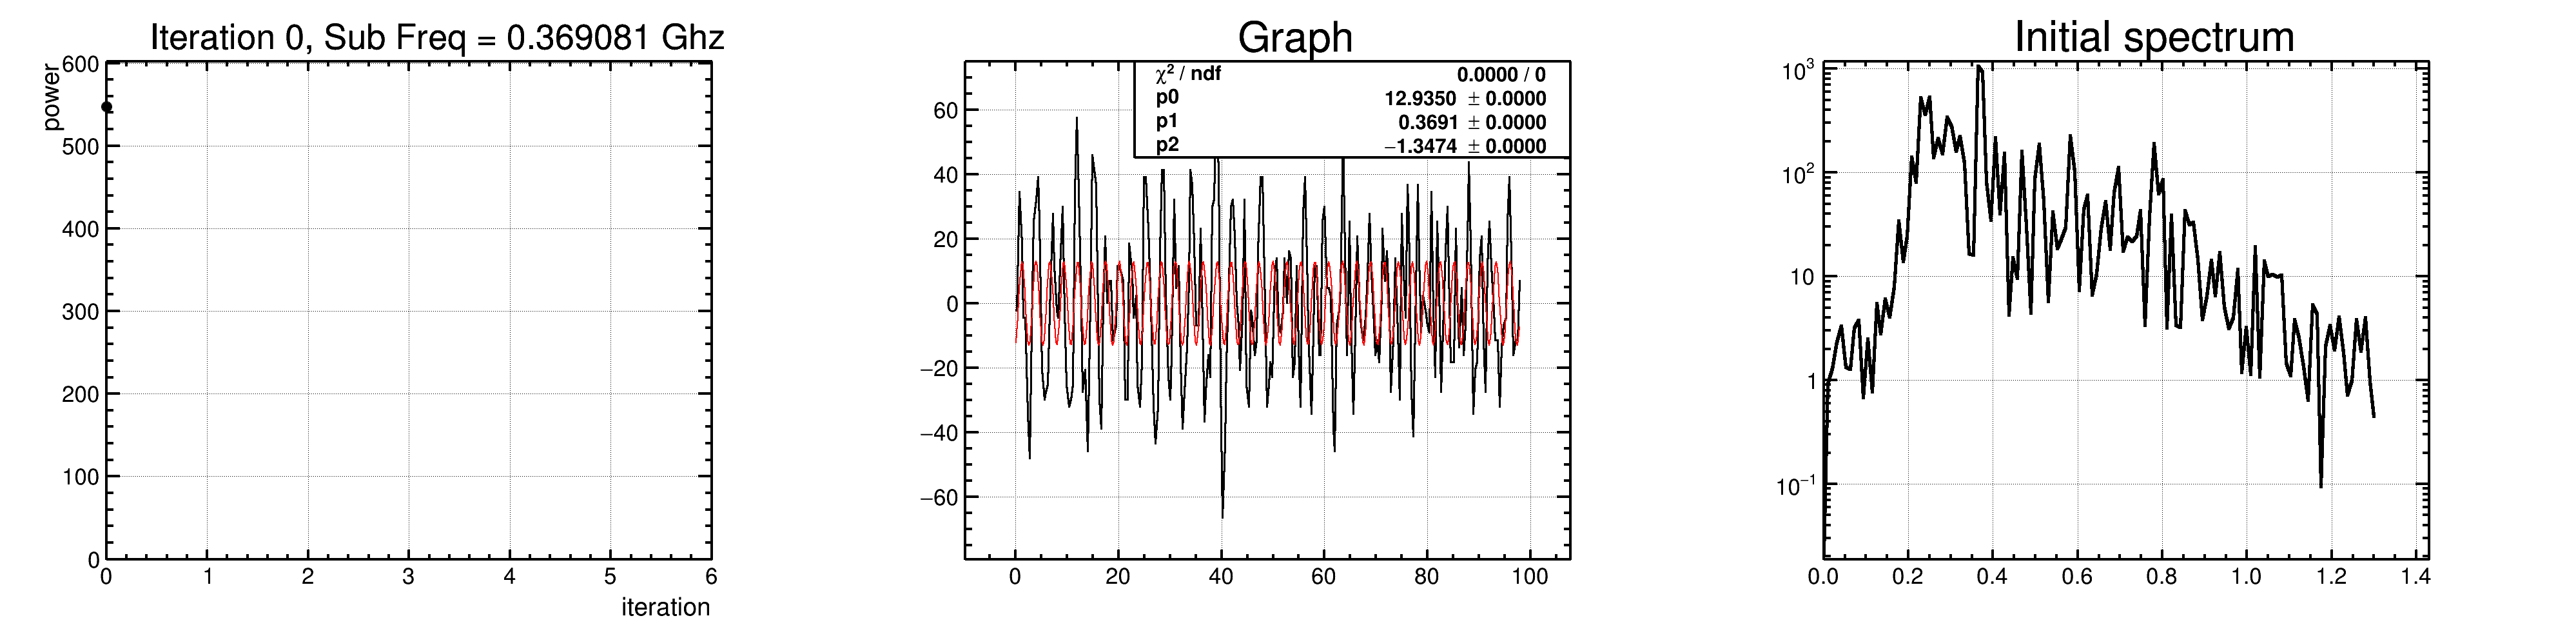
\includegraphics[height=0.13\textheight]{figures/sineSubtract_0}		
	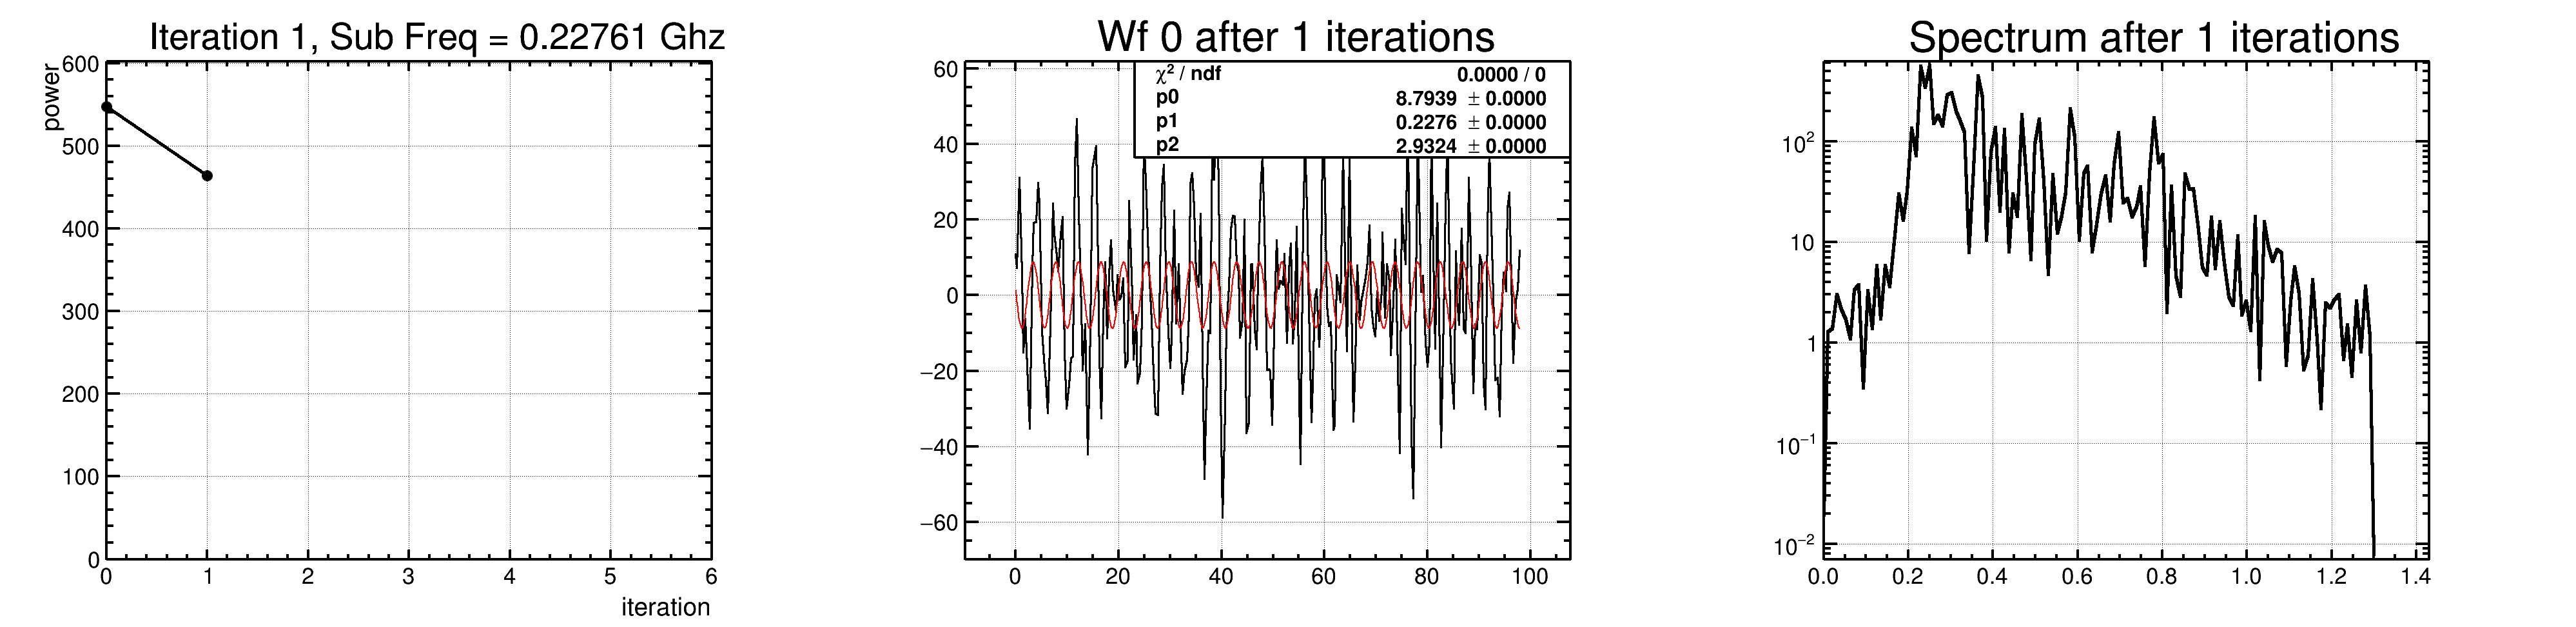
\includegraphics[height=0.13\textheight]{figures/sineSubtract_1}
	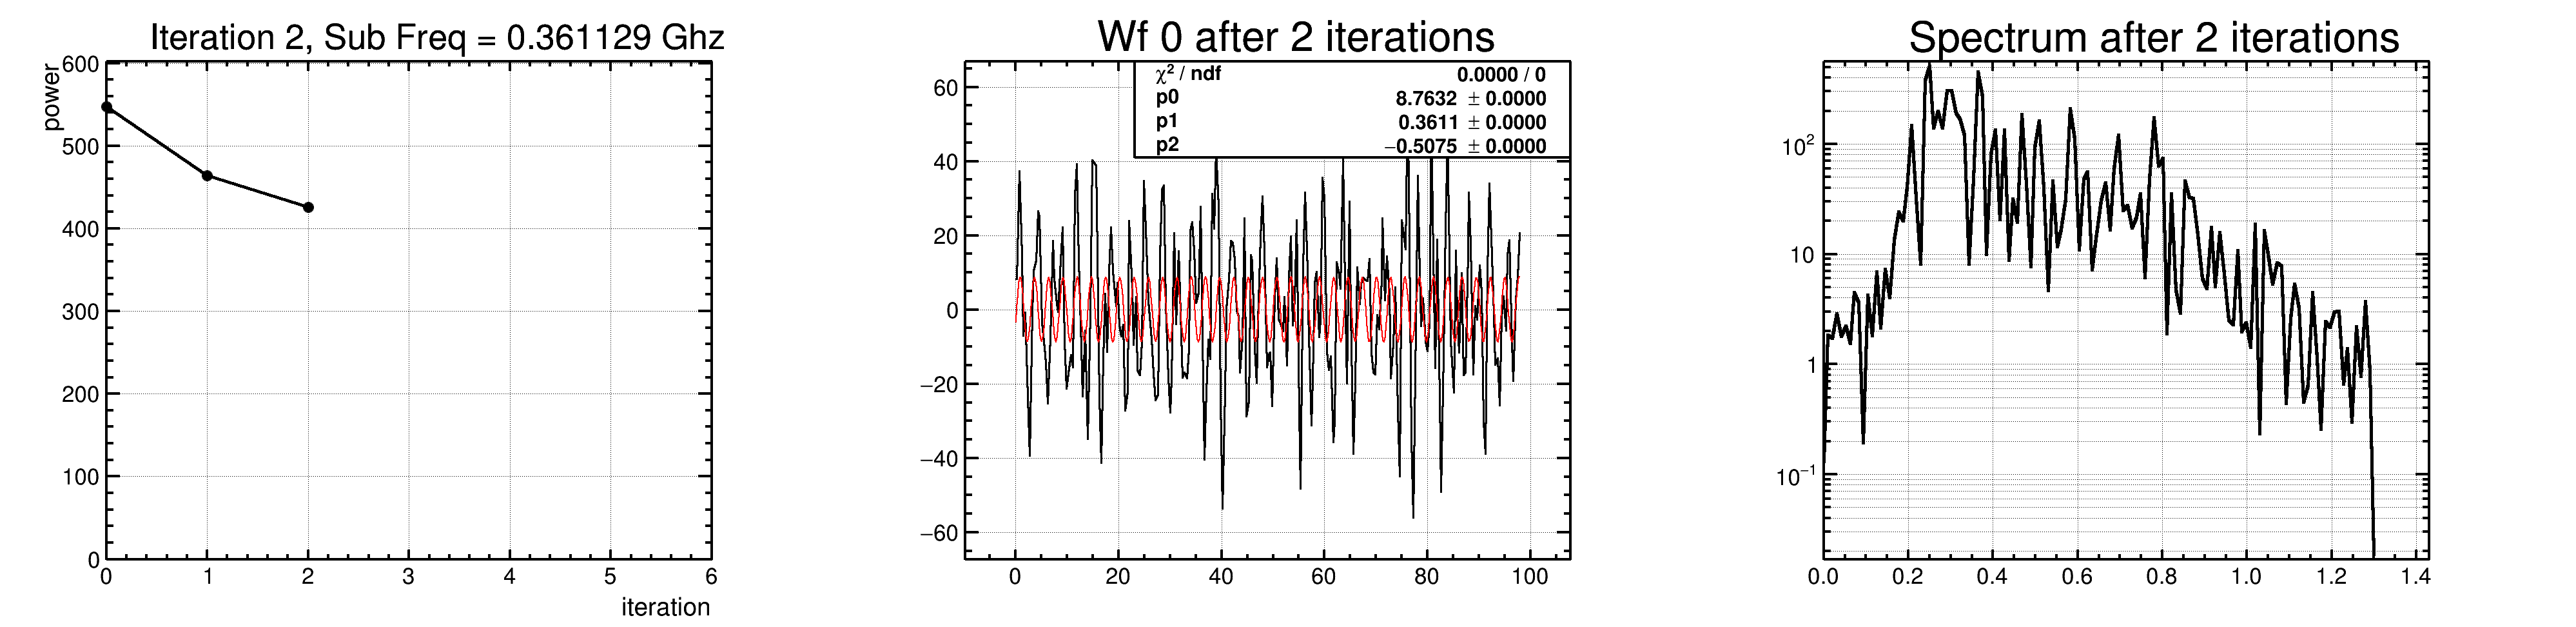
\includegraphics[height=0.13\textheight]{figures/sineSubtract_2}
	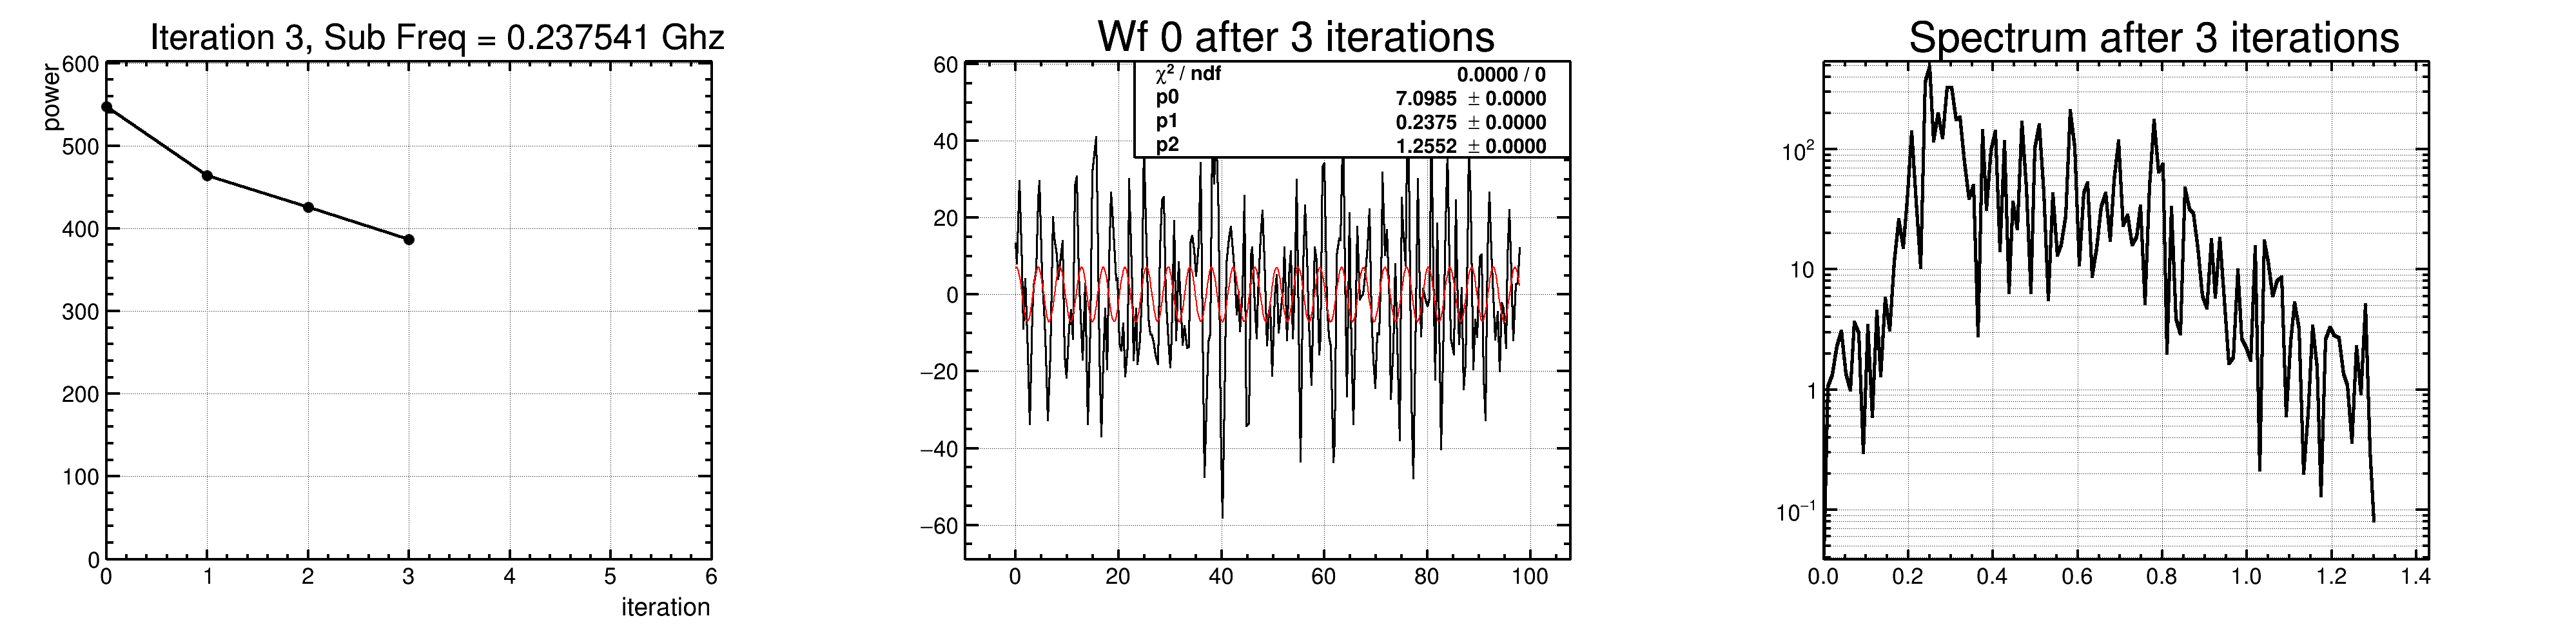
\includegraphics[height=0.13\textheight]{figures/sineSubtract_3}
	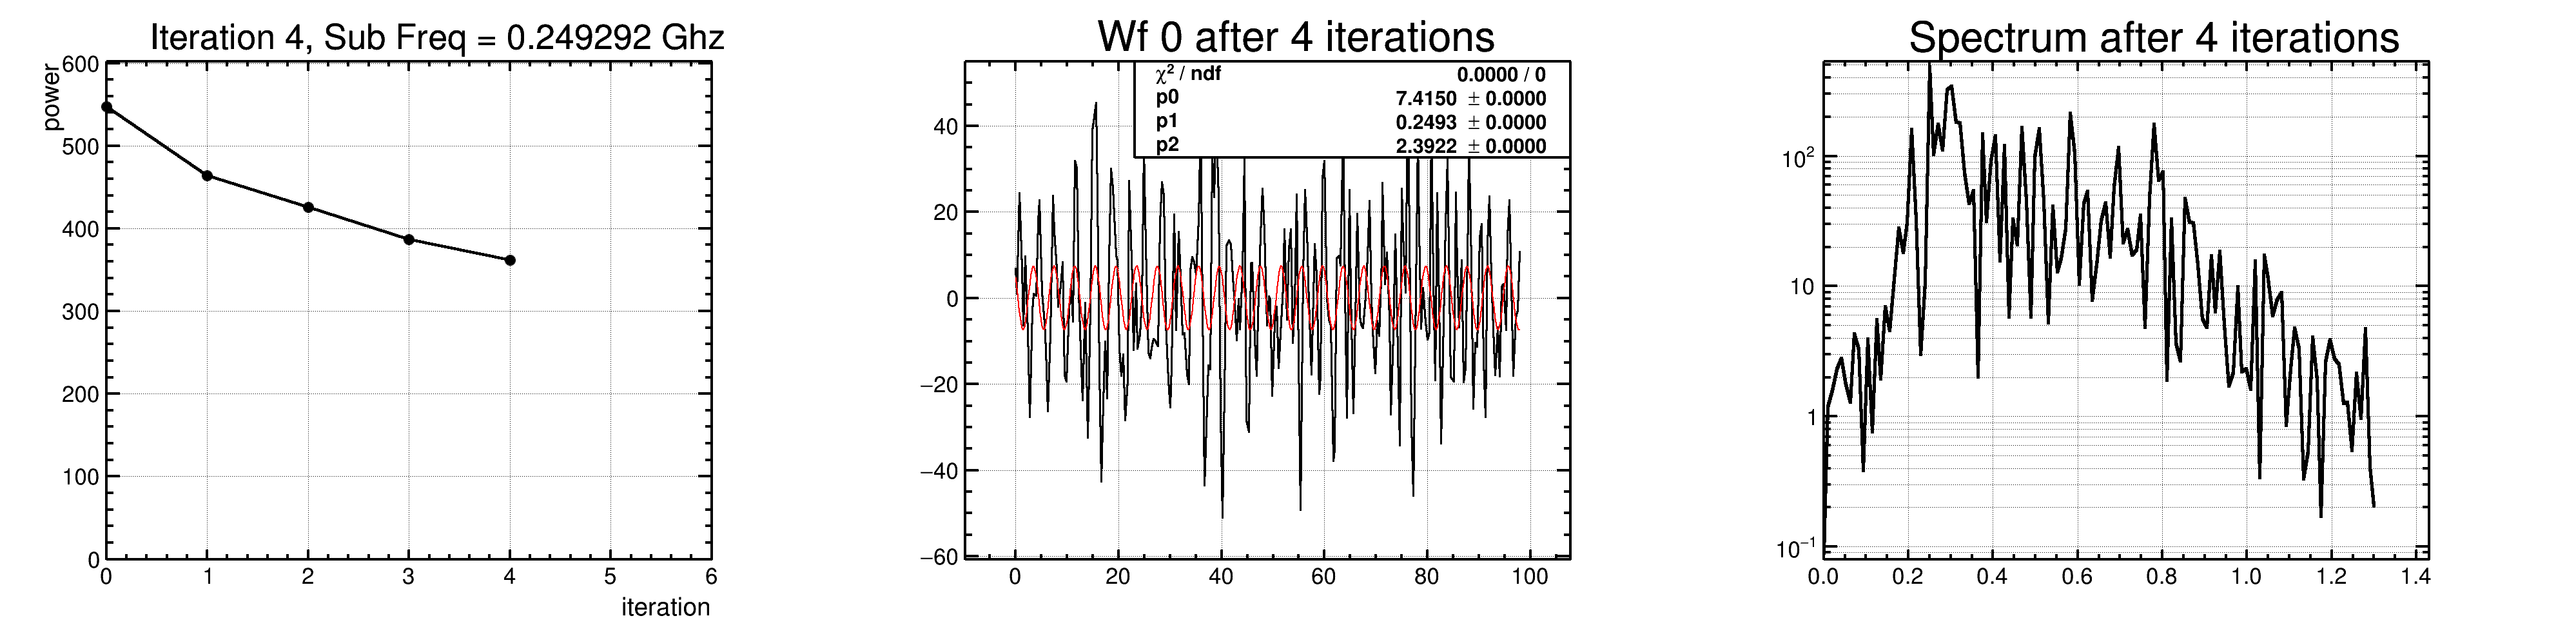
\includegraphics[height=0.13\textheight]{figures/sineSubtract_4}
	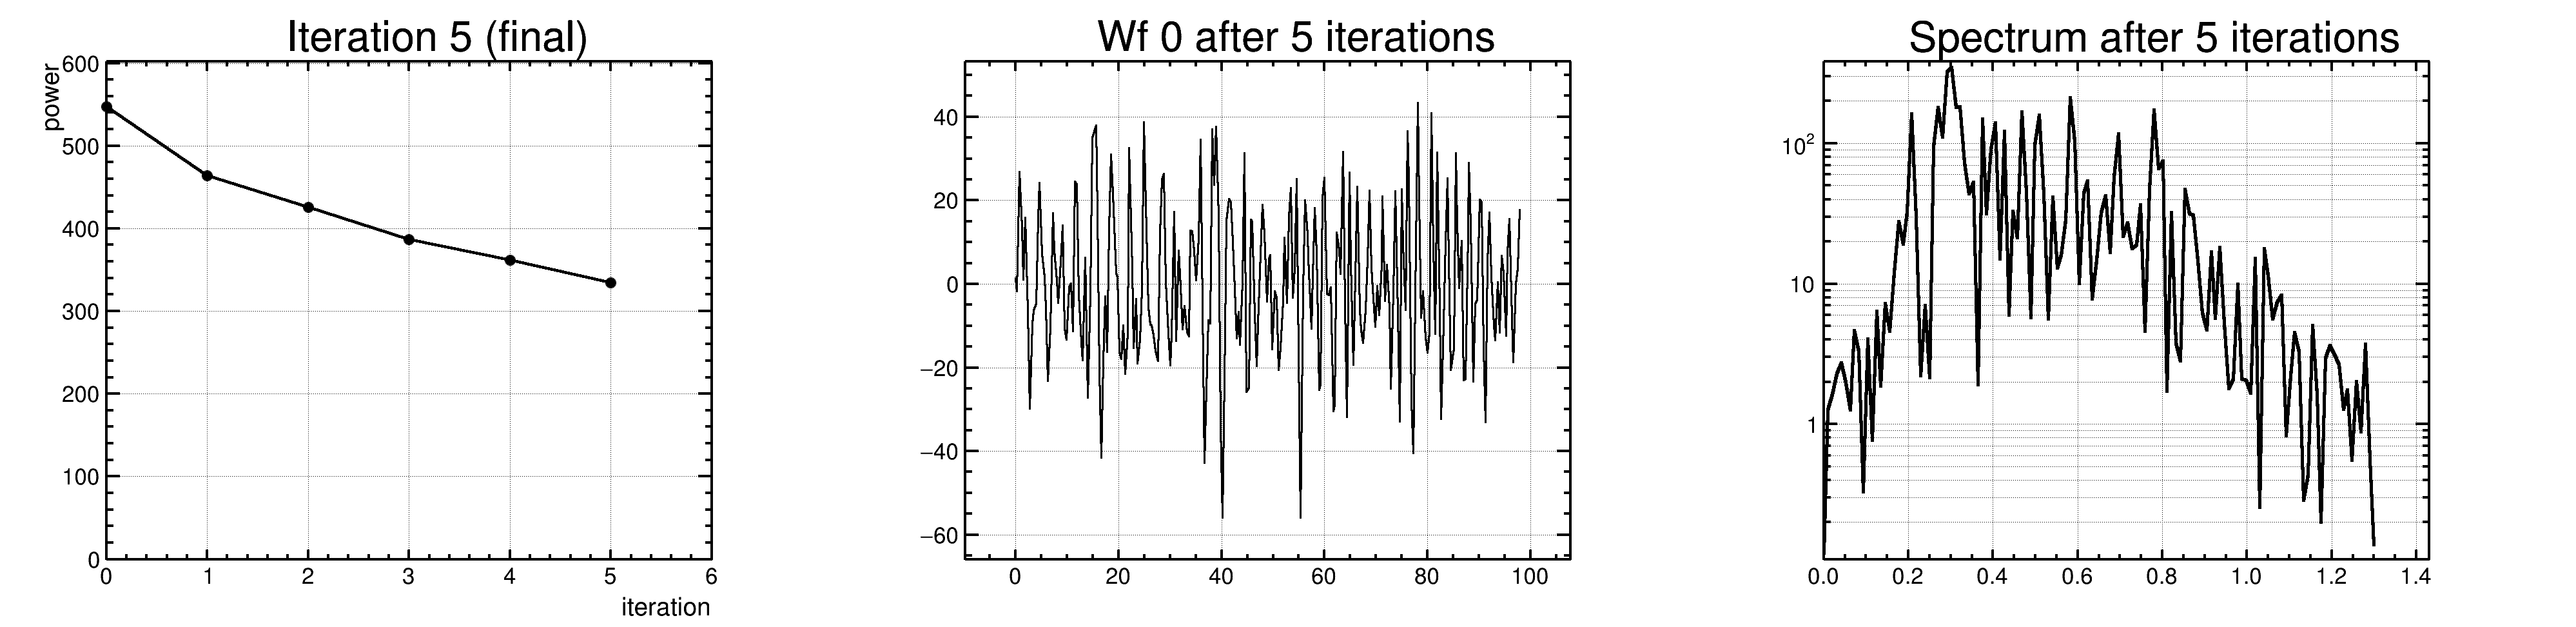
\includegraphics[height=0.13\textheight]{figures/sineSubtract_5}
	\caption{The effect that sine subtraction filtering has on a single waveform for event 56765803.  The top-most set of plots is the initial waveform, and the bottom-most set is the final ``filtered'' waveform. (Left) The amount of power removed per iteration.  (Middle) In black is the waveform used for the fit, and in red is the fit sine wave function.  Also visible are the final fit parameters.  From top to bottom they are the amplitude, frequency (in GHz), and phase.  (Right) The spectral power of the corresponding waveform prior to the sine wave being subtracted.} 
	\label{fig:SineSubtractExample}
\end{figure}

\section{Waveform Reconstruction}%5
	To extrapolate the measured signal on the ANITA instrument back to a physics signal or background noise event, we must combine the various waveforms captured around the instrument.  By summing the values various waveforms with specifically determined time offsets, it is possible to determine the level of coherence of the electromagnetic environment.  Once an arrival direction is determined it is possible to reconstruct the signal, averaging out the random thermal and electronic noise.
	
	By correlating the waveforms captured between various antenna pairs it is possible to establish time delays in which multiple channels maximally constructively interfere.  Known as interferometry, a radio astronomy technique, it makes use of the known physical separation vector between the antennas and the propagation delay for any incident plane wave.\cite{interferometry}  By overlaying the correlation values for multiple baselines, it is possible to generate a map of likely pointing directions.  ANITA has three vertical tiers of antennas, each separated from each other, and at least three co-pointing phi sectors that are expected to observe events from any angle.  Using the combined baseline offsets from these antennas, it is possible to overlay 9 different interferometric maps to create a pointing map.  By finding the peak of this map, a vector pointing away from the payload can be traced to the ice, where a map of the vertical height of the continent can be used to create a map of events on the ground.
	
	\subsection{Interpolation}
		As discussed earlier, the waveforms have a nominal sampling rate of 2.6GS/s, yielding a mean timing separation of 385ps.  This presents an issue, namely that baseline timing delays between antenna pairs are not quantized in multiples of this value.  In order to accurately overlay the recorded waveforms of different channels, upsampling the signal to a higher rate with a lower time separation between points is required.  Additionally, the variation in time separation between samples caused by process parameter spread in the LABRADOR ASICs presents computational difficulties for Fourier analysis of signals.
		
		There are several methods that can take unevenly sampled waveforms as an input, and output an evenly sampled approximation of the signal by extrapolating between points, a process called interpolation.  An Akima spline iteratively fits a cubic polynomial to a range of sampled points, then uses that fit to determine the intermediate points.  Akima splines do a good job at determining an equivalent evenly sampled waveform, but introduces spectral distortion when used for increasing the sampling frequency.  Another method of interpolation, which I'll call Fourier domain upsampling, computes the complex Fourier transform of a waveform, appends zeros to the end until the desired frequency is reached, then calculates the inverse Fourier transform of that extended frequency domain signal.  This method introduces no in-band spectral distortion, though for computational simplicity it must be performed on an evenly sampled waveform.  A comparison of these two methods in interpolating a raw, 2.6GS/s, unevenly sampled LAB output waveform to an evenly sampled 10GS/s waveform is shown in Figure \ref{fig:interpolation}.
		
		The methodology used in this thesis for interpolation is to use an Akima spline to evenly sample the recorded waveforms, then using the Fourier domain upsampling technique to increase the sampling rate by a factor of three, to 7.8GS/s.
		
\begin{figure}
\centering
	\includegraphics[width=0.9\textwidth]{sigChain_upsample}
	\caption{An example from channel 01BH of even resampling and up-sampling the original unevenly sampled LABRADOR digital readout.  The peak of the impulse is shown zoomed, while a view of the entire waveform can be seen in the inset frame showing the macro-consistency of the methods.  The method used in this analysis is  FFT up-sampling.  Despite undershooting some points, it minimally distorts the spectral power and phase response of the signal.}
\label{fig:interpolation}
\end{figure}		
	
	\subsection{Radio Interferometric Mapping}
		Interferometric mapping is a method developed to compare measured time domain waveforms captured by antennas with a physical baseline offset with the goal of determining likely incoming plane wave direction.\cite{interferometry}  This is accomplished by calculating the timing offsets expected from each direction of a pair of antennas in elevation and azimuth, computing the correlation function of the two waveforms, then building an interferogram by weighting each direction in relation to the correlation value at that specific timing offset.  The number of unique permutations for $N$ antennas choosing two at a time is given by the binomial coefficient, shown in Equation \ref{eqn:binomial}
		
	\begin{equation}
	{{N}\choose{2}} = \cfrac{N!}{2(N-2)!}
	\label{eqn:binomial}
	\end{equation}
		
		For the analysis inthis theis, $N=15$ antennas were used, yielding 105 baseline pairs per map point.  An example of four antennas yielding six single baseline pairs and the subsequent interferometric map can be seen in Figure \ref{fig:mapCreation}.
		
\begin{figure}
\centering
	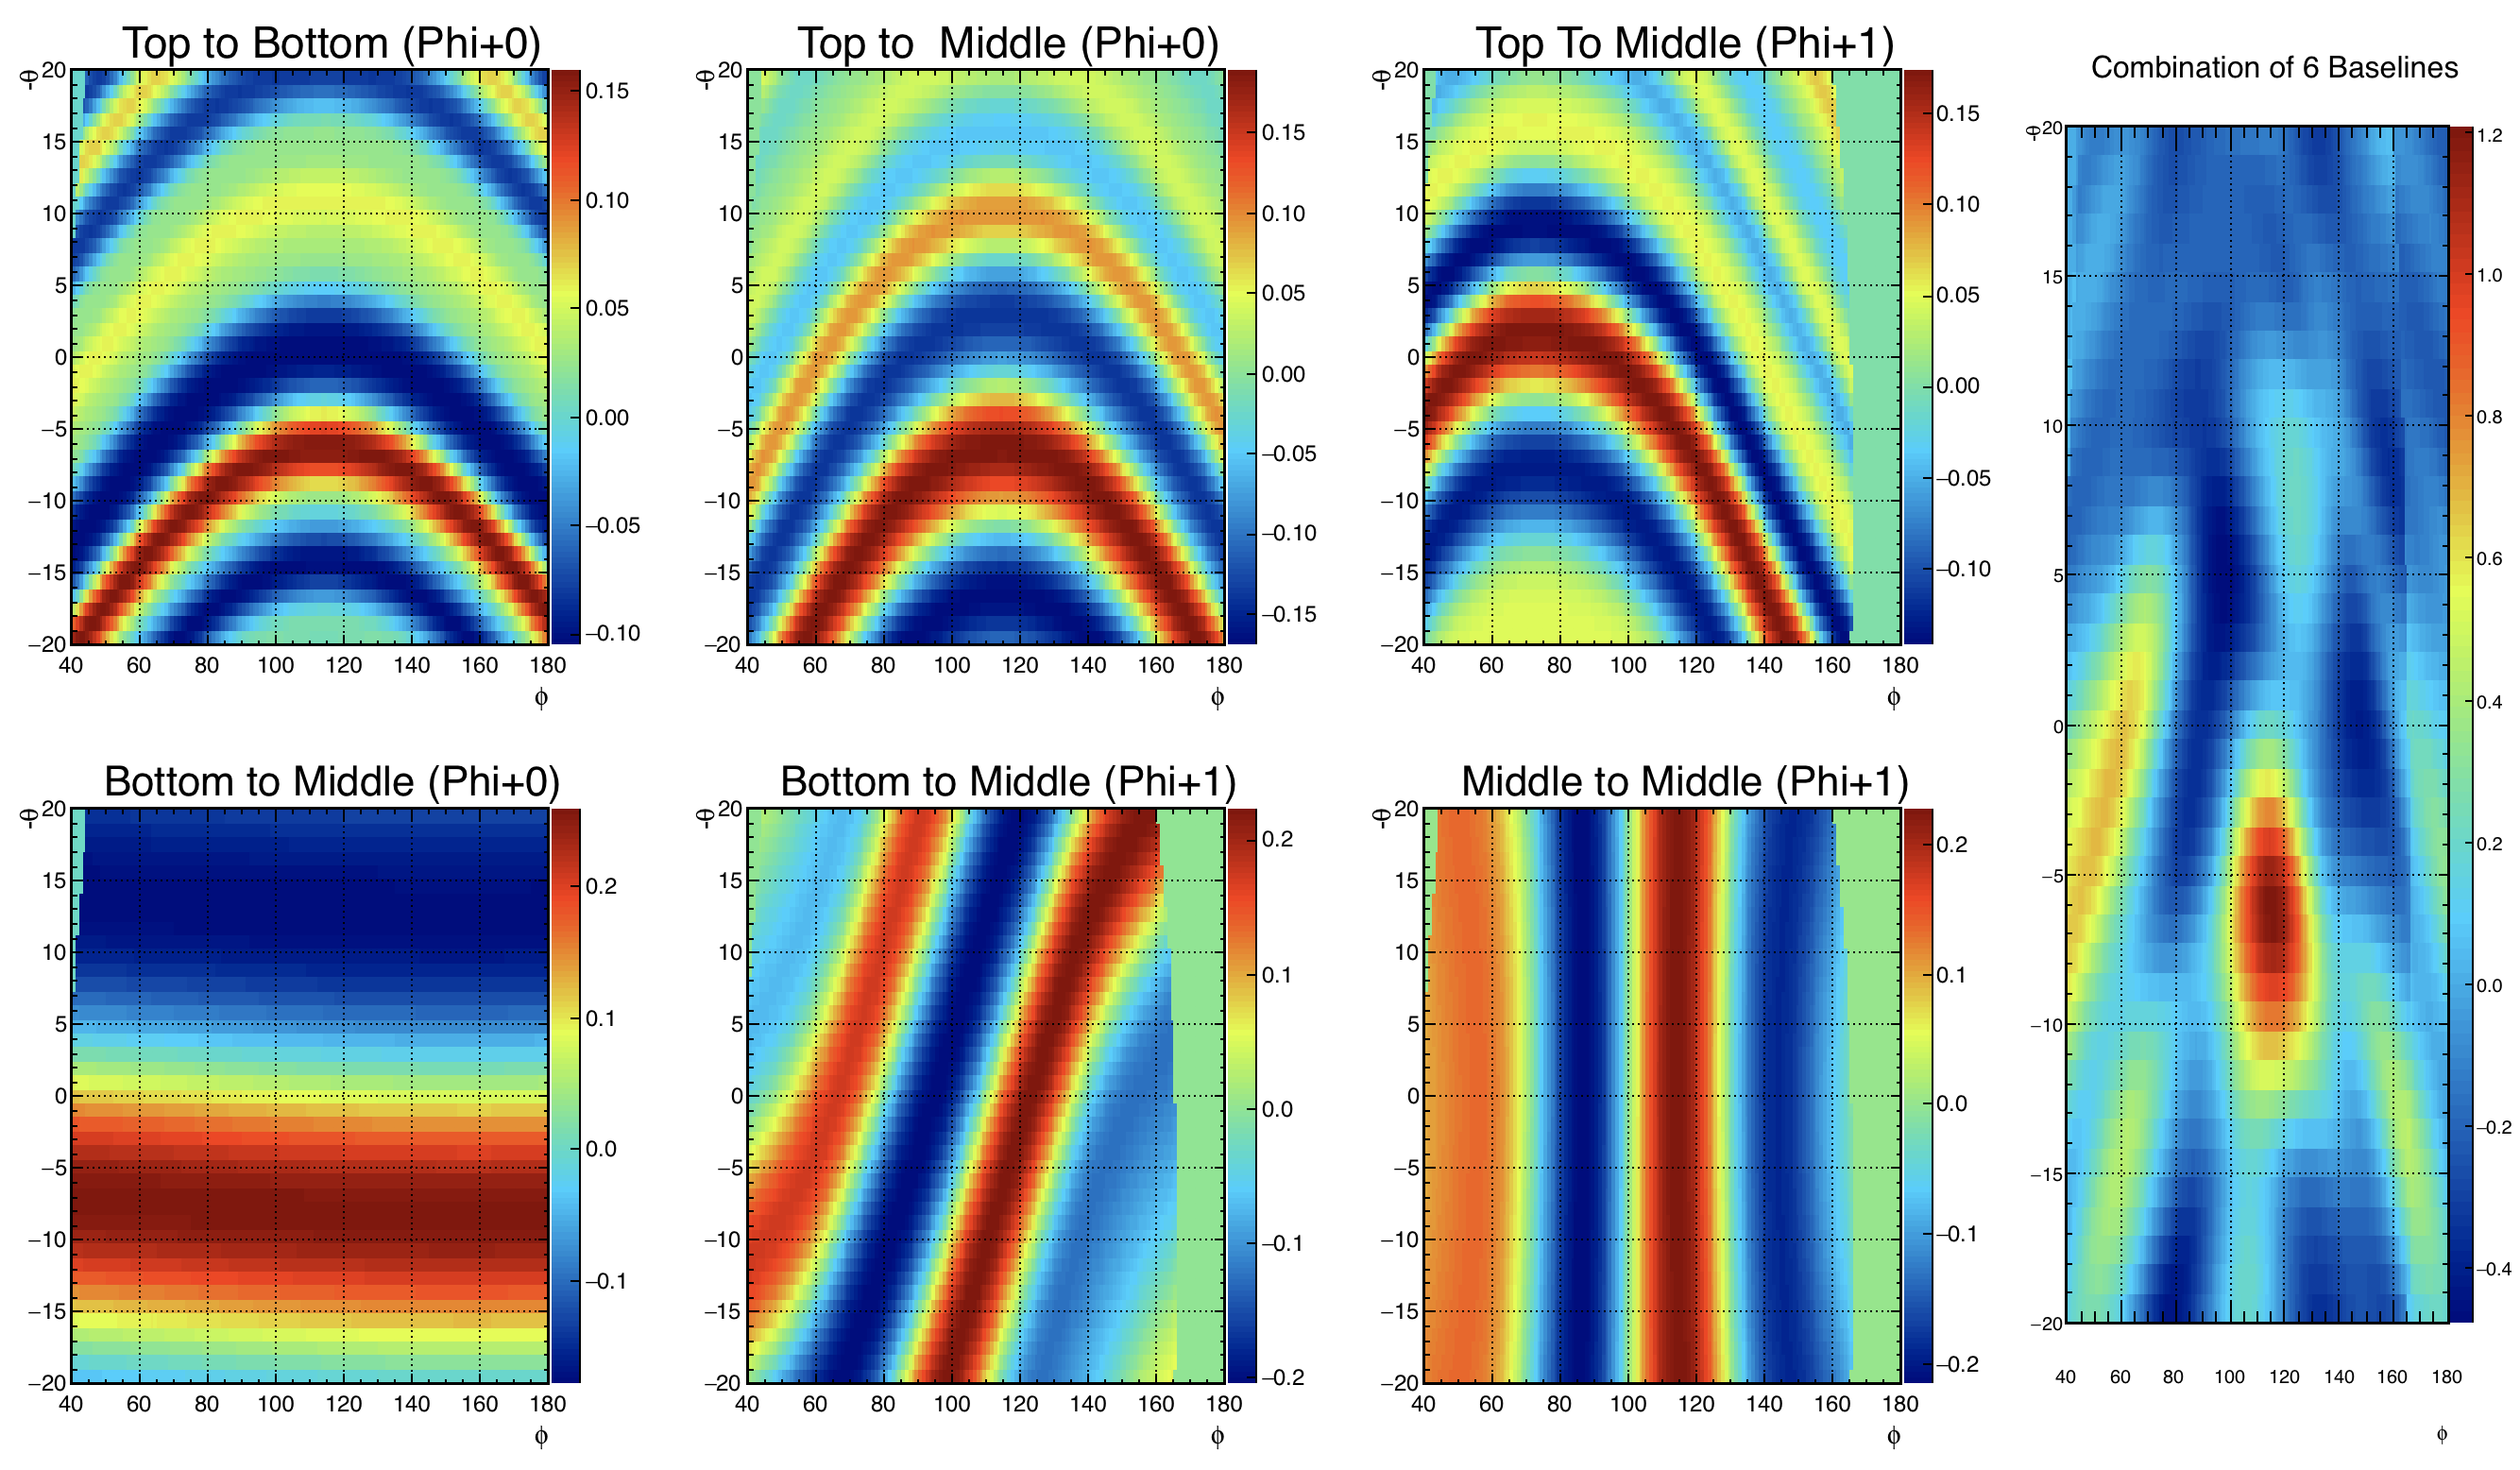
\includegraphics[width=0.9\textwidth]{interferometricMapCreation}
	\caption{Six interferograms for single baseline correlation offsets between four antennas, and their combined full interferometric map.  The signal being reconstructed for this image is a WAIS pulser event.  The four antennas used are all three in the phi sector pointing nearest the incident pulse, as well as the middle ring antenna in the neighboring phi sector.  Maps created in the full analysis combine interferograms from 15 antennas}
	\label{fig:mapCreation}
\end{figure}
		
		
	\subsection{Coherent Waveform Sum}
		The electronic and thermal noise present in each channel limits the sensitivity of the instrument to EAS signals with low power.  Since the power within the radiation of an EAS shower varies linearly with the energy of the particle, low energy showers, which have a higher flux rate, will have signal to noise ratios approaching one.  Additionally, polarization information and frequency content are effected by any noise present in the system.  Averaging waveforms from multiple channels will reduce this incoherent background noise by a factor of $\sqrt{N}$.  After determining the peak interferometric pointing direction, it is possible to align the channels that received signal from an incident radiation field and average them together.  An example of this is shown in Figure \ref{fig:coherentSum}.
		
		For this analysis 15 antennas, comprising 5 phi sectors, are used to construct the coherently summed waveform.  The 15 antennas are chosen based on the peak of the interferometric map, so that the closest 5 phi sectors are included.  
		
		The waveforms are then delayed based on the physical offsets between the phase centers of the antennas and a zero-point defined at the center of the payload, and added together with that timing offset preserved.  This preserves the absolute timing information of the signal, since all coherently summed waveforms will have the same reference point.
		
		
	\subsection{Signal to Noise Ratio (SNR)}
		The Signal to Noise Ratio (SNR) is a measure of the ratio of powers between the coherent signal present in the waveform  and the average noise power of that same waveform.  This value is calculated by dividing the average of positive peak ($V_+$) and negative peak $(V_-$) voltages of the coherently summed waveform, and dividing it by an average of the root mean squared (RMS) of the  past one minute of minimum bias waveforms for the channels that are used in the coherent sum.  Equation \ref{eqn:SNR} describes this calculation.
		
	\begin{equation}
	SNR = \frac{V_{+}-V_{-}}{\sum^{60}_{i=0} V_{rms,i}}
	\label{eqn:SNR}
	\end{equation}
	
	In this thesis when I refer to SNR, I mean the value that is calculated from the voltage and timing calibration signal as stored to disk.  This includes the dispersion of the signal chain and antennas, as well as the additional cascaded electronic noise introduced by the amplifiers.  The SNR of the incident electric field will have a different value.
	
	
	\subsection{Ray Tracing to Continent}
		 The location that an interferometric map peak points to on the ice can be determined by tracing a vector pointing in the peak direction back to the continent.  To do this, it is important to have an accurate topographical map of both the Earth's surface, as well as the ice sheet that covers it.  These maps are provided by the Radarsat Antarctic Mapping Project Digital Elevation Model Version 2(RAMPDEMv2)~\cite{RAMPDEM}.  RAMPDEMv2 provides topography as referenced to the geoid model of the earth.  Without a correct topological information, events would point to areas that are shadowed from view by mountainous terrain.  An example of pointing to various topographical models, and description of the technique, are shown in Figure \ref{fig:traceBackToContinent}
		 
\begin{figure}
	\centering
	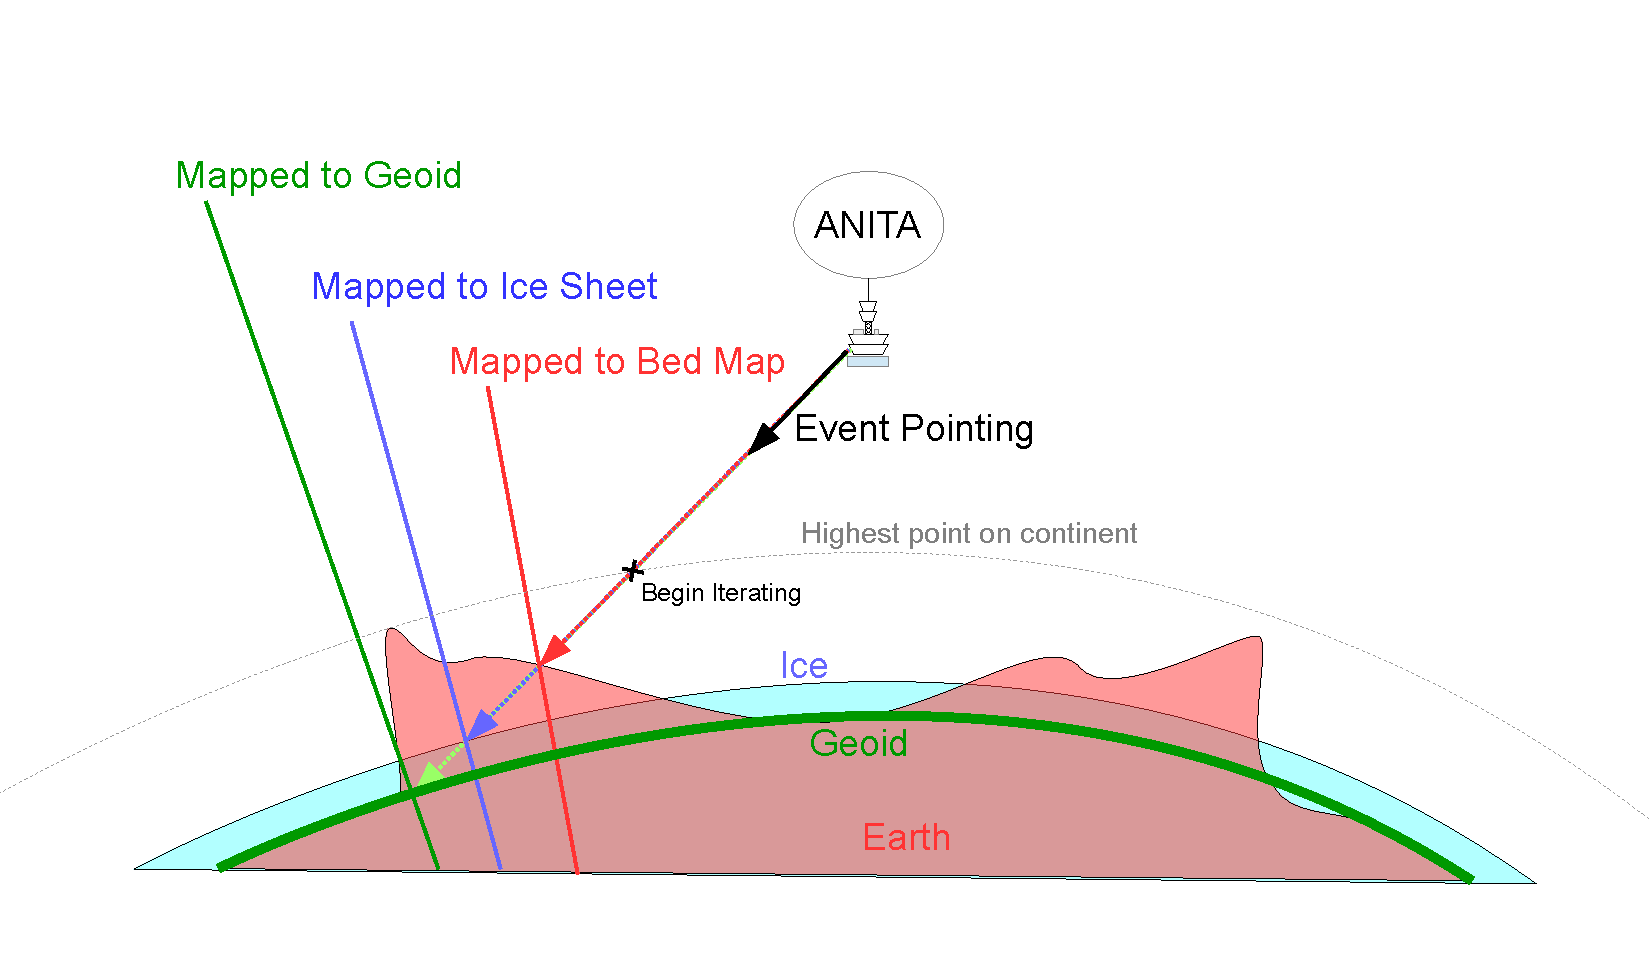
\includegraphics[height=0.5\textheight]{figures/traceBackToContinent}
	\caption{A diagram showing how events are traced back to the continent.  First the latitude and longitude of an event at the highest altitude on the continent (Mt. Vincent at 5000m) is determined.  Then the vector is iteratively lengthened until it intersects with a topographical dataset provided by RAMPDEMv2.  This is done for both a map of ice field heigh, and a bedrock map.  The latitude, longitude, and altitude trace back to the continent is then saved for the event for the top two peaks.} 
	\label{fig:traceBackToContinent}
\end{figure}	 
		
	\subsection{Immediate Pointing Cuts}
		Real physics signals have a small range of elevation angles where their detection is most likely.  The highest probability incident direction for an EAS is near the horizon, however noise events will point more evenly in all directions.  Using this knowledge, we can cut out events that have very steep elevations.  A distribution of event pointing direction can be seen in Figure \ref{fig:elevationAngle}.

\begin{figure}
	\centering
	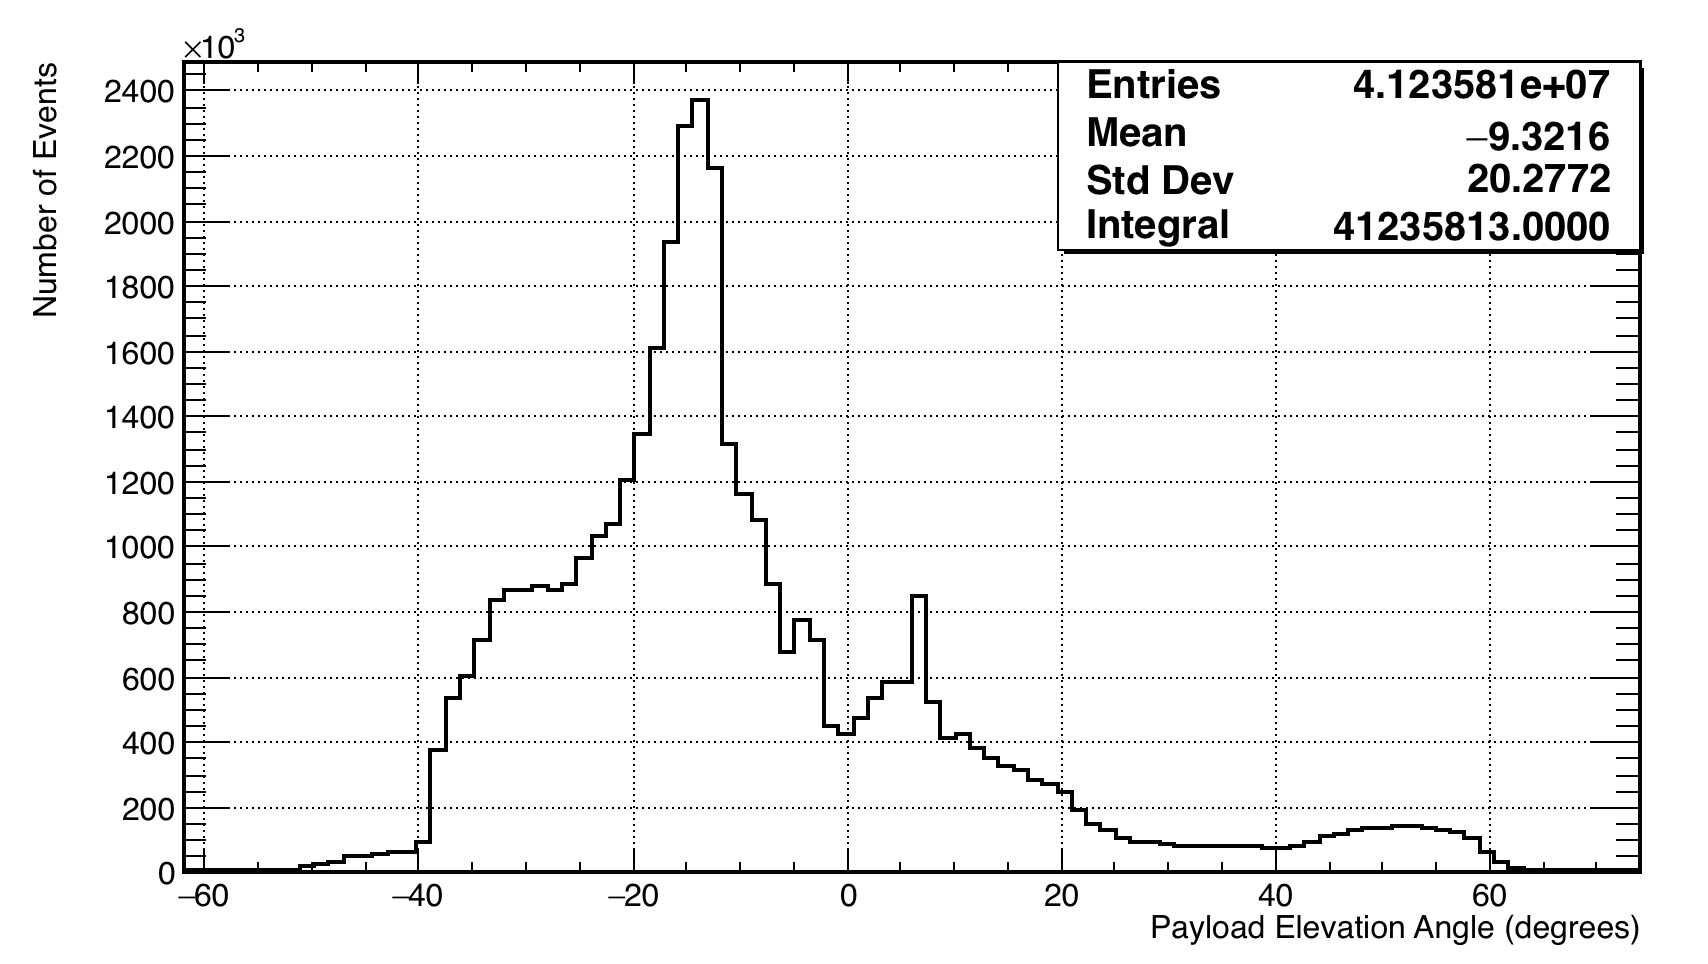
\includegraphics[width=\textwidth]{figures/elevationAngle}
	\caption{The distribution of elevation angles of the first interferometric peak for all waveforms.  Zero points perpendicular to the vertical payload vector, and negative values denote events that point ``downwards'' from the payload.  The horizon, which depends on surface height and payload altitude, has an average value of around -6 degrees.  The most common source above the horizon is the sun.} 
	\label{fig:elevationAngle}
\end{figure}	 
		


\section{De-dispersion}%6
	The antenna, filters, cables, and amplifiers are responsible for introducing a frequency dependent gain and group delay to the observed signals.  These elements act to disperse the power in the signal across tens of nanoseconds from what was emitted from the relativistic shower at the critical angle as a highly impulsive, picosecond length essential delta-function like electromagnetic field transient.  The impulse response, or complex phasor representation of this dispersive effect, was measured for the signal chain immediately preceding the flight for each of the 96 channels, and for all 48 antennas in a controlled manner in Palestine the summer beforehand.  These two effects are then combined and used to determine a whole system impulse response that relates the measured ADC values at the LABRADOR digitizer to an electric field incident at the payload.  By reversing the dispersive process, via Weiner deconvolution (described below), we can both increase the instantaneous power of a signal and compare it directly to the electric field radiation output of high energy particle shower simulations such as COREAS or ZHAires.


	\subsection{Generation of transfer function}
		The transfer function of the system was painstakingly developed and utilized a variety of both time domain and Fourier transformed frequency domain manipulations.  These each introduce their own errors, as many of them require assumptions about the incoming signal.  I detail the full process of generating the transfer function in Appendix A.


	\subsection{Signal to noise ratio of impulse response}
		Any band limited deconvolution process requires a knowledge of the signal to noise ratio of the transfer function as a function of frequency ($SNR(f)$).  Since the transfer function merely relays the amplitude and phase differences between an input and output signal (represented in either a complex phasor or a time domain waveform), one must also have an understanding of the total power contained within the input and output signals.  If, for example, both the input and output signal contained very little power out of a specified band pass, it could be wrongly assumed from a transfer function that the signal chain was able to pass frequencies that are out of the band pass.
		%The "signal" and "noise" of this must therefore be defined, as the spectral power has multiple sources.  
		
		
	\subsection{All-Pass Deconvolution}
		The impulse response used to deconvolve waveforms has been colloquially named the All-Pass deconvolution method.  An ideal deconvolution, one that uses both phase and amplitude information to remove the instrument response, is poorly defined outside the instrument bandwidth.  Since the instrument blocks any signal outside this frequency range, reversing the procedure introduces what is in essence a "divide by zero" error that grossly amplifies signal power outside the band.  The simplest way to avoid this is to disgard the frequency dependent amplitude information, and only correct for the phase.  Due to the relatively flat spectral response of the ANITA system, this is a good first approximation.  The resulting waveform "stacks" signal power from all in-band frequencies on top of one another, increasing the observed peak to peak signal to noise ratio and offering a larger separation between signal and noise events during analysis cuts.



\section{Template Correlation}%7
	Though any physics experiment that aims to separate background events from signal events requires that a general understanding of characteristics inherent to either group, measurements and simulations of UHECR induced EAS signatures provide a waveform template that can be used to strongly cut on signal events.  The simplest assumption, that an EAS will produce a broad spectrum, short duration, electromagnetic pulse, drives both the overall design of the payload, as well as several of the analysis cuts.  Determining a normalized correlation between a template and the coherently summed waveform provides an additional constraint beyond simply requiring impulsivity, and also requires that the gain and phase characteristics of an incident wave are in agreement with an EAS signal.

	\subsection{ZHAires Shower Modeling}
		Simulating the radio emission of cosmic ray air showers is accomplished by using the ZHS extension to the AIRshower Extended Simulations (AIRES) package.\cite{AlvarezMuñiz2012325}  Concatenated, these two packages make up the ZHAires simulation framework.  This framework, developed by Jaime Alvarez-Muniz, Washington Rodrigues de Carvalho Jr. and Enrique Zas, generates a time varient electric field for a configurable incident particle at some instrumentation point in the atmosphere.  Recent work, with ANITA specifically in mind, has further extended the simulation to accurately depict reflections off the ice sheet.
		
		Simulations provide an important method to determine the overall sensitivity of the ANITA instrument to air shower events as a function of incident angle, energy, and payload location.  Due to the coherent beamed characteristic of air shower radio emmission, specifically a peak at the critical Cherenkov angle from the shower axis, ANITA is only sensitive to a small fraction of showers that occur within its field of view.
		
		The spectral content of EAS radiation falls off sharply as a function of offset from the critical Cherenkov angle.  Without being within a few degrees of the peak coherence angle, low frequency radiation, below the band of the ANITA instrument, dominates the spectrum.  This was shown in Figure \ref{fig:EASSignalPower}

	
	\subsection{Templates}
		It is possible to generate several different templates that accurately represent an observable EAS signal on the payload.  Additionally, templates can be developed from averaging together calibration pulser or other anthropogenic signals of interest.  For this analysis, the template used for a cut value was a simulated EAS electric field measured at 0.175 degrees outside the critical coherence angle, convolved with the instrument impulse response.  Figure \ref{fig:templates} shows a comparison between the 9 CR templates, as well as the impulse response template and averaged WAIS pulser template.  The WAIS pulser template was used to establish cut efficiency on WAIS pulses, as they do not have the same phase structure as EAS signals.
		
\begin{figure}
	\centering
	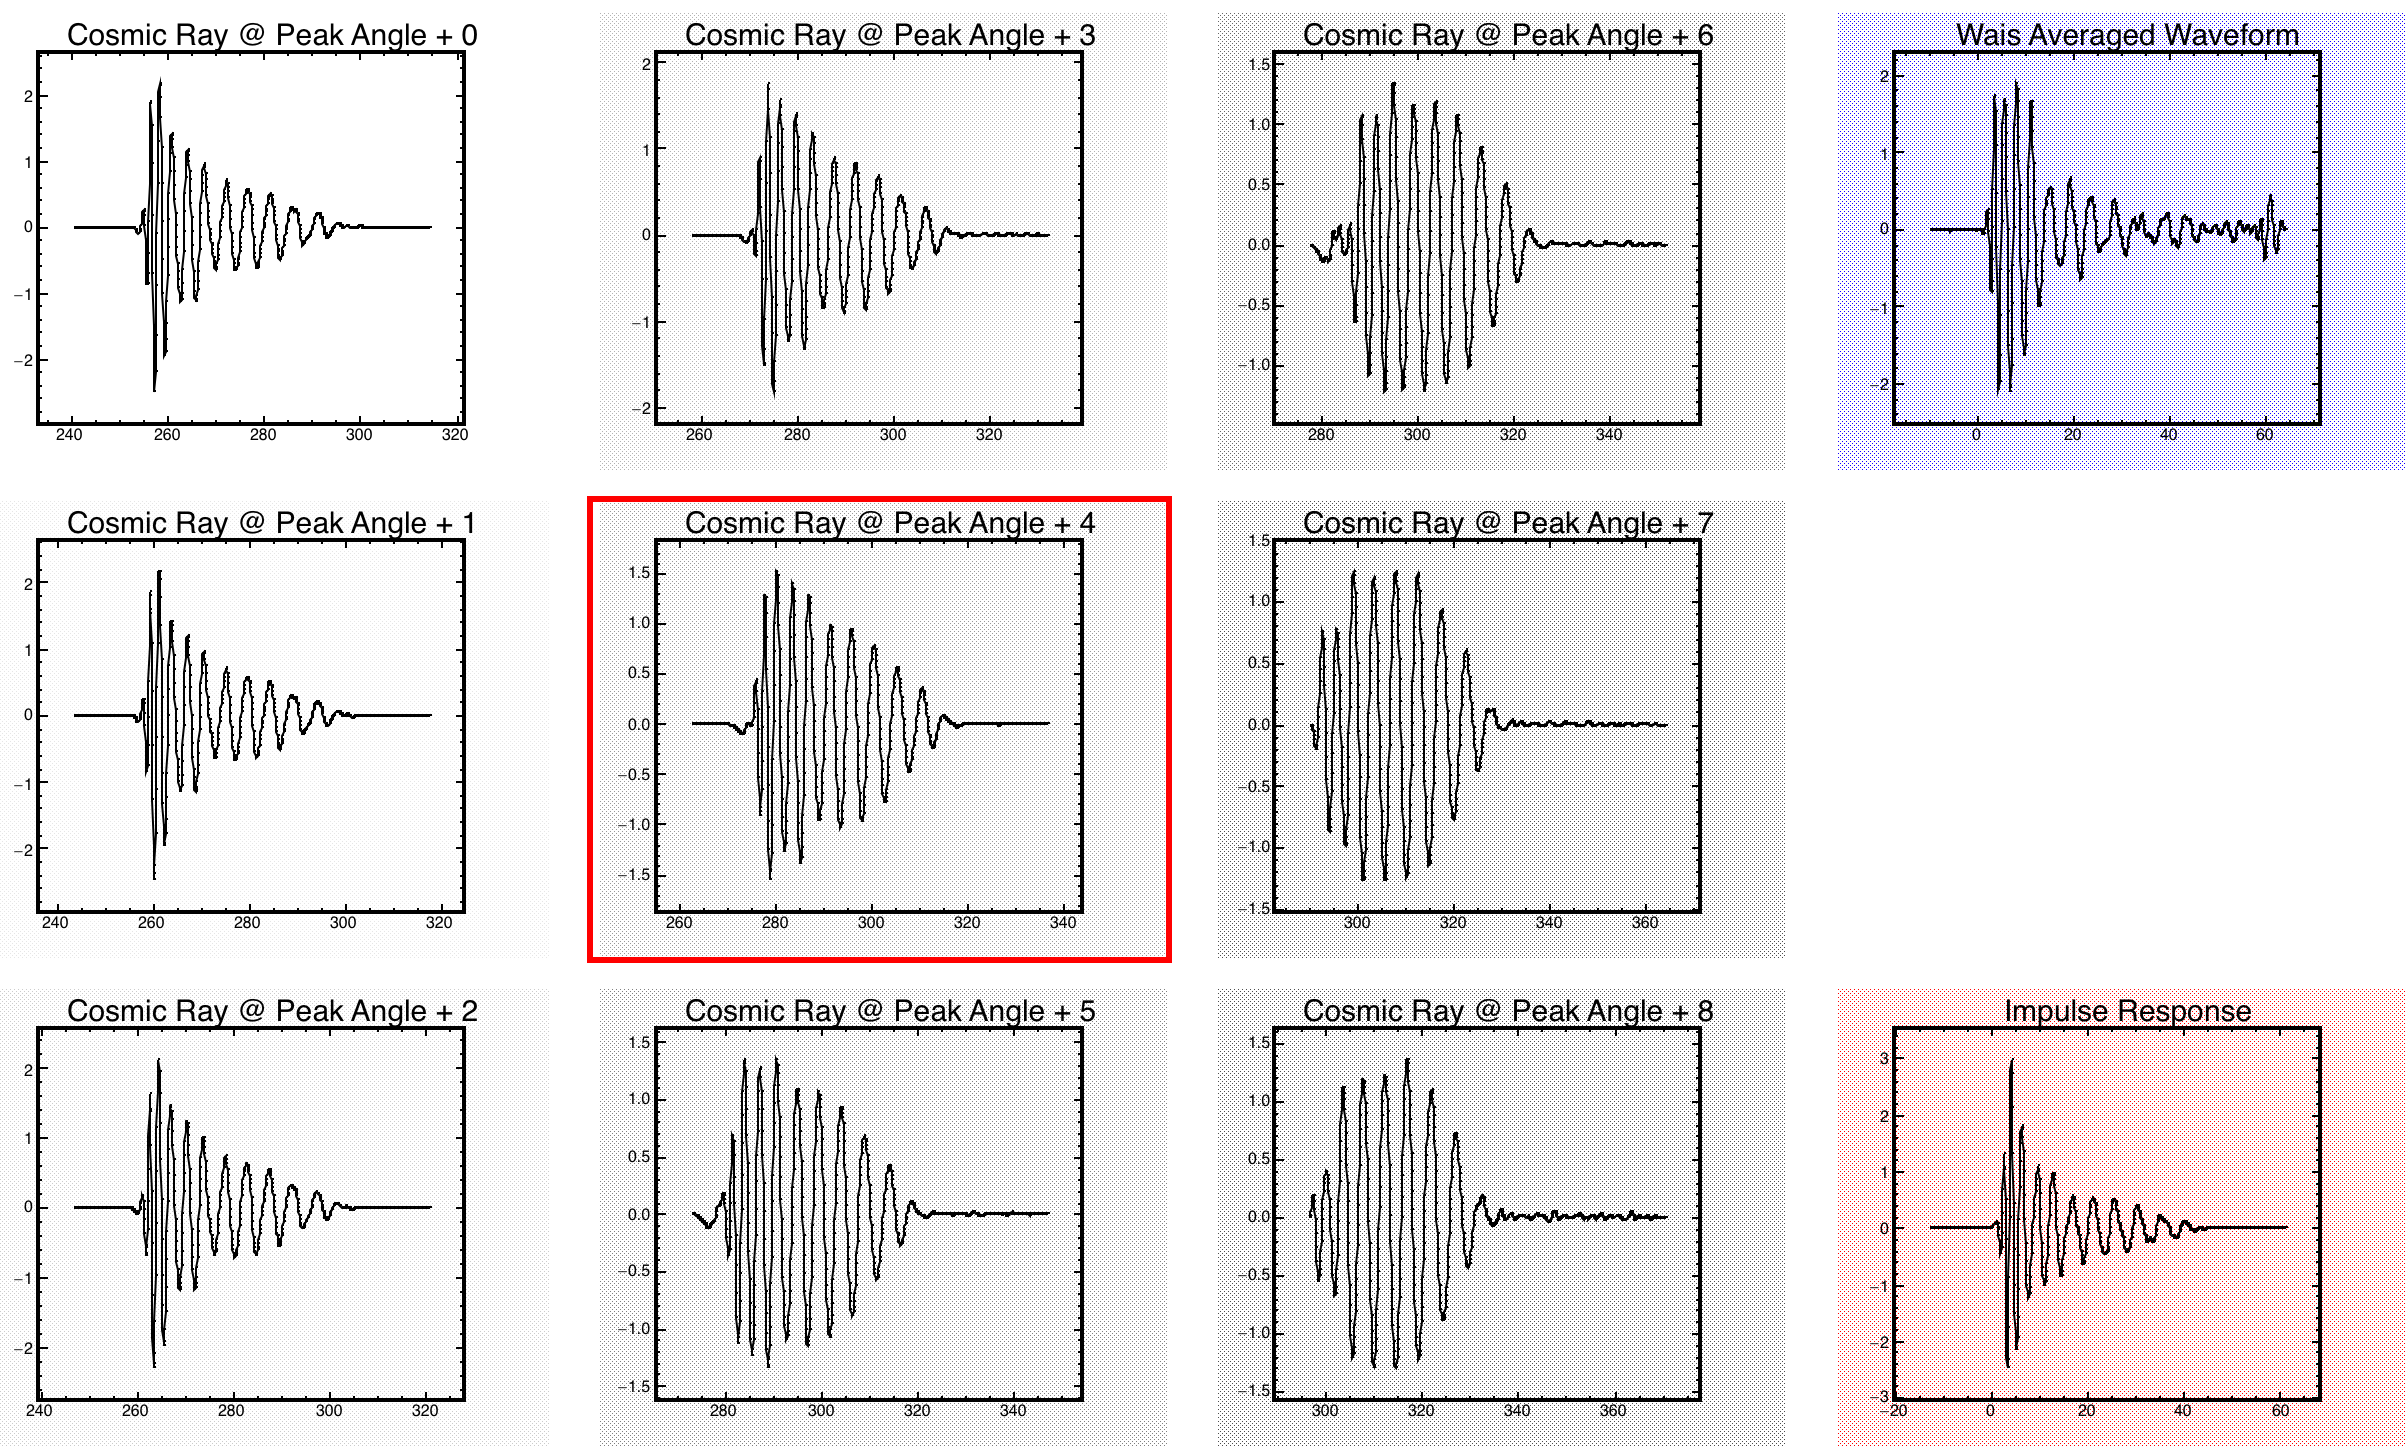
\includegraphics[width=\textwidth]{figures/templates}
	\caption{The 11 templates used in this analysis.  The leftmost 9 templates were generated from ZHAires simulations convolved with the system impulse response. The center waveform, in the red box, was used for setting cuts for the analysis.  The peak coherence angle for this simulated shower occurred at 0.675$^{\circ}$ from the shower axis, and each waveform was measured at steps of 0.04$^{\circ}$ from that peak.  The top right is a template derived by correlating and averaging 10,000 WAIS pulser events, and is used for determining reasonable cut parameters based on calibration pulser efficiency.  The bottom right is the impulse response of the system.  All waveforms are normalized so that their autocorrelation is one.} 
	\label{fig:templates}
\end{figure}		
		
		
	
	\subsection{Auto-correlation normalization}
		In order to make the template correlation value of different events directly relatable to one another, it is important to normalize both the template and the coherently summed waveform.  As this measurement is most interesting in determining the amount that any given event ``looks'' like the template, the final value should be a fraction from 0 to 1, where 1 would be a waveform that is an exact copy of the template.

	\subsection{Issues with filtering}
		Ideally these templates would be compared against the coherently summed waveforms that have been filtered for CW interference on a channel by channel basis.  However, the distortion of the phase structure induced by all of the filtering strategies, including sine subtraction, reduces the correlation to values below that of un-filtered waveforms.  For this reason, only the template correlation value for unfiltered coherently summed waveforms is used.

\section{Polarization cuts}%8
	The expected signal from a cosmic ray air shower has a characteristic polarization that can be used as a further discriminator between random noise, which will have a random polarization.  Specifically, the geomagnetically induced radiation component will be linearly polarized and orthogonal to both the shower axis and the magnetic field.  This allows two cuts to be made, one of the linear polarization fraction and one of the linear polarization angle.  Both these rely on the calculation of Stokes parameters made possible by the dual polarization antennas, which capture both these time domain electric fields simultaneously.

	\subsection{Stokes Parameters}
		The Stokes parameters are a mathematical method for describing the polarization of electromagnetic radiation with a four-vector of values.  The four parameters in the Stokes vector are $I$, which describes the total intensity, $V$ which describes the circular polarization, and $U$ and $Q$, which describe the linear polarization in two rotated bases.  $Q$ corresponds to linear polarization in coordinate basis that is either parallel or perpendicular to the complex electric field measurements, and $U$ is the basis rotated $45^{\circ}$ from that.  A visual representation of the Stokes parameters is shown in Figure \ref{fig:Stokes}.  These values can be determined for each digitized event by comparing the temporally dynamic electromagnetic fields of the orthogonally positioned Hpol and Vpol channels from each antenna.  The equations for calculating these values are shown in Equation \ref{eqn:Stokes}.
		
	\begin{gather*}
	\varepsilon_{i} = E_{i} + i\hat{E}_{i} \\
	I =	\frac{1}{n}\sum^{n-1}_{0}(|\varepsilon|^{2}_{i,H} + |\varepsilon|^{2}_{i,V}) \\
	Q =	\frac{1}{n}\sum^{n-1}_{0}(|\varepsilon|^{2}_{i,H} - |\varepsilon|^{2}_{i,V}) \\
	U =	Re(\frac{1}{n}\sum^{n-1}_{0}(\varepsilon_{i,H} \varepsilon_{i,V}*)) \\
	V =	Im(\frac{1}{n}\sum^{n-1}_{0}(\varepsilon_{i,H} \varepsilon_{i,V}*)) \\
	\label{eqn:Stokes}
	\end{gather*}

		
	 $\hat{E}$ is the Hilbert transform of the electric field waveform, $E_{H}$ is the signal from the horizontally oriented antenna channel, and $E_{V}$ is the vertically polarized signal.  The $i$ is the sample number from the evenly spaced waveform.  $\varepsilon$ is then the complex voltage of the signal, where $i=\sqrt{-1}$.  $Re$ and $Im$ denote taking the real or imaginary part of the value, and $*$ is the complex conjugate operator.  This equation has axes referenced to the horizontal, perpendicular to the vector normal to the Earth. \cite{PhysRevD.94.103010}
	 
	 To reduce the effect that background noise has on the calculation of the Stokes vector, the waveform was truncated after 500 points ($n=500$ in Equation \ref{eqn:Stokes}), or 50ns after the beginning of the coherently summed waveform.  This was chosen to capture the entirety of measured WAIS calibration pulses, but remove the trailing edge.
	 
	 Determining the uncertainty on the calculation of these values was done by calculating the Stokes parameters for each waveform used in the coherent sum and determining the spread of the distribution of calculated values around the value calculated for the coherent sum.
	 
	\subsection{Linear Polarization Fraction}
		The fraction of the signal that is linearly polarized can be calculated using Stokes Parameters.  The $Q$ and $U$ components of the vector represent the linearly polarized portions of the signal, which can be normalized to the total coherent radiation $I$ and added in quadrature to determine the fraction of power that is linearly polarized, $L$, as shown in Equation \ref{eqn:LinPolFrac}.
		
	\begin{equation}
		L=\sqrt{U^2 + Q^2}
	\label{eqn:LinPolFrac}
	\end{equation}
		
	It is expected that signal-like events will be mostly linearly polarized, while incoherent thermal sources will have low values of $L$.  This can be used as a cut parameter for a cosmic ray search.  The distribution of $L$ for events that pass quality cuts can be seen in Figure \ref{fig:LinPolFrac_goodEvs}.
	
	\begin{figure}
	\centering
	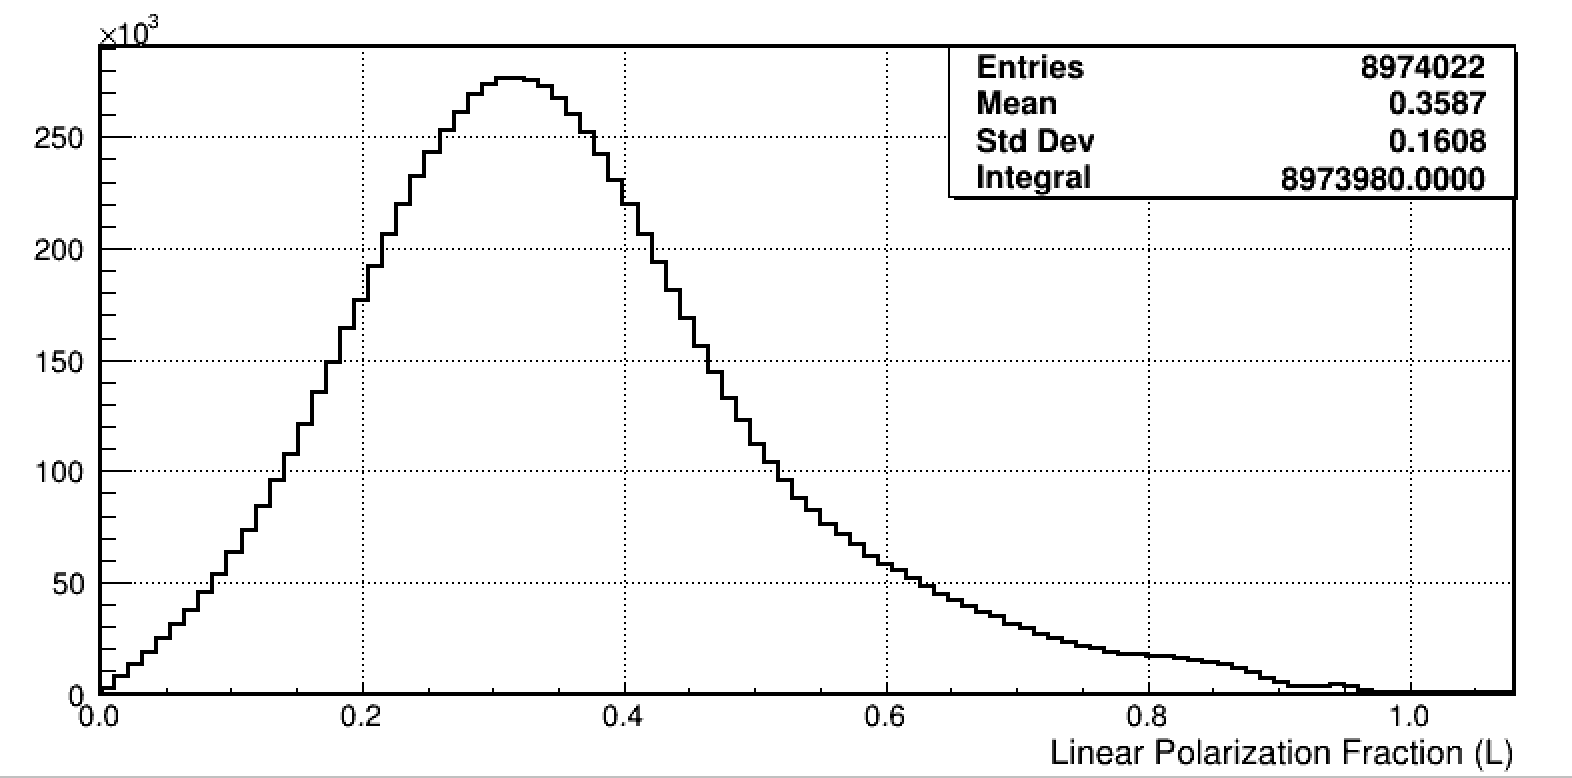
\includegraphics[width=\textwidth]{figures/linPolFrac_goodEvs}
	\caption{The distribution of linear polarization fraction for events measured during the ANITAIII flight that pass quality cuts.  As expected, the majority of events are thermal in nature, and have low measured values of $L$.} 
	\label{fig:LinPolFrac_goodEvs}
\end{figure}
	
	
	\subsection{Total polarization fraction}
		The two major contributors to CR induced EAS radiation, radially polarized Askaryan and linearly polarized Geomagnetic, can combine to create a signal with a circularly polarized element.  It is therefore useful to calculate the total polarization fraction of the measured events.  Since $U$, $Q$, and $V$ all measure components of polarized coherent radiation, the quadrature sum of the total coherent radiation normalized parameters gives the total polarization fraction $I_{p}$, shown in Equation \ref{eqn:Ip}.
		
	\begin{equation}
		I_p = \sqrt{(\frac{U}{I})^2 + (\frac{Q}{I})^2 + (\frac{V}{I})^2}
	\label{eqn:Ip}
	\end{equation}

		Equation \ref{eqn:Ip} simplifies to Equation \ref{eqn:Ip2}.
		
	\begin{equation}
		I_p = \frac{\sqrt{U^2 + Q^2 + V^2}}{I}
	\label{eqn:Ip2}
	\end{equation}

		This 
	\subsection{Plane and angle of linear polarization}
		The predominant geometric plane of linearly polarized radiation is referred to the plane of polarization.  The angle between the horizontally polarized antenna electric field axis and this plane is the linear polarization angle, and will be denoted by $\Psi_{L}$.  This angle can be calculated by computing the angle between projections of the $U$ and $Q$ Stokes parameters onto their corresponding coordinate bases, shown in Equation \ref{eqn:polAngle}.
	
	\begin{equation}
		\Psi_{L} = \frac{1}{2}tan^{-1}(\frac{U}{Q})
	\label{eqn:polAngle}
	\end{equation}
		
		Since the convention of the sign of the polarization of the signal is a matter of definition, for simplicity the values of $\Psi_{L}$ are restricted to angles between $0^\circ$ and $90^\circ$.
		
	\subsection{Expected vs measured geomagnetic polarization angle}
		The expected linear polarization angle of radiation emitted by an EAS will correspond primarily to the cross product between the shower axis and the geomagnetic field vector at the shower maximum.  Comparing the expected and measured polarization angle for observed isolated impulsive events can be used as a final discriminator on the likelihood that they are from an astrophysical interaction.  
		
		Calculating this expected angle requires a knowledge of the pointed event location on the continent of Antarctica, its reconstructed incidence elevation angle, and the geomagnetic field at the location in the atmosphere where shower max occurred.  Additionally, a majority of detectable EAS events will have reflected off the ice sheet of the continent, requiring the the calculation to include the Fresnel reflection coefficients for components of the incident radiation Poynting vector perpendicular and parallel to the ice-air boundary.  This reflection also inverts the polarity of the parallel components of the electromagnetic field.
		
		Up-going tau neutrino candidates are also expected to be dominated by linearly polarized geomagnetic radiation, however the location of the shower maximum will be above the ice sheet between the pointed source location and the payload.  These events will then have different expected geomagnetic polarization angles than if the event was a reflected down-going cosmic ray induced extensive air shower.  In order to preserve both astrophysical signals in the final candidate list, the expected geomagnetic angle is calculated for both cases, and the measurement falling close to the expectation of either case is treated as sufficient to pass cuts.
		
		
\section{Polarity Estimator}%9

	In order to identify up-going tau neutrino candidates within the detected cosmic ray candidate set, it is important to have a method for determining the sign of the polarity for any particular event.  Since a reflection off the ice will invert the polarity of the electromagnetic field impulse, it is clear that an event with a steep elevation angle but polarization that is inverted from the bulk of the CR candidates will be from an astrophysical particle exiting the continent and creating a shower within the atmosphere.
	
	The polarity estimation for this thesis was accomplished by determining whether the absolute value of the peak of the correlation is the maximum or minimum, i.e. if the sign of the peak is negative or positive.  Since detection of a tau neutrino would be both exciting and controversial, the mis-identification of this method is desired to be as small as possible.  The sign of the peak of the correlation is recorded for both the coherently summed and the de-dispersed waveforms.  When this method is applied to the 118,268 tagged WAIS pulser events, which all have the same polarity, only one was identified as the incorrect polarity by using the coherent sum, a misidentification rate of $8.46\times10^{-6}$.  However, using the de-dispersed waveform, 200 events (including the single mis-identified event from the coherent sum) were found, a misidentification rate of $1.69\times10^{-3}$.  This is shown graphically in Figure \ref{fig:waisPolarity}.  To be considered properly identified, the estimates for the dispersed and coherent waveforms are required to be identical.  This yields 1 ($8.46\times10^{-6}$) WAIS event that is mis-identified, and 199 ($1.68\times10^{-3}$) events of indeterminate polarity.
	
		
\begin{figure}
	\centering
	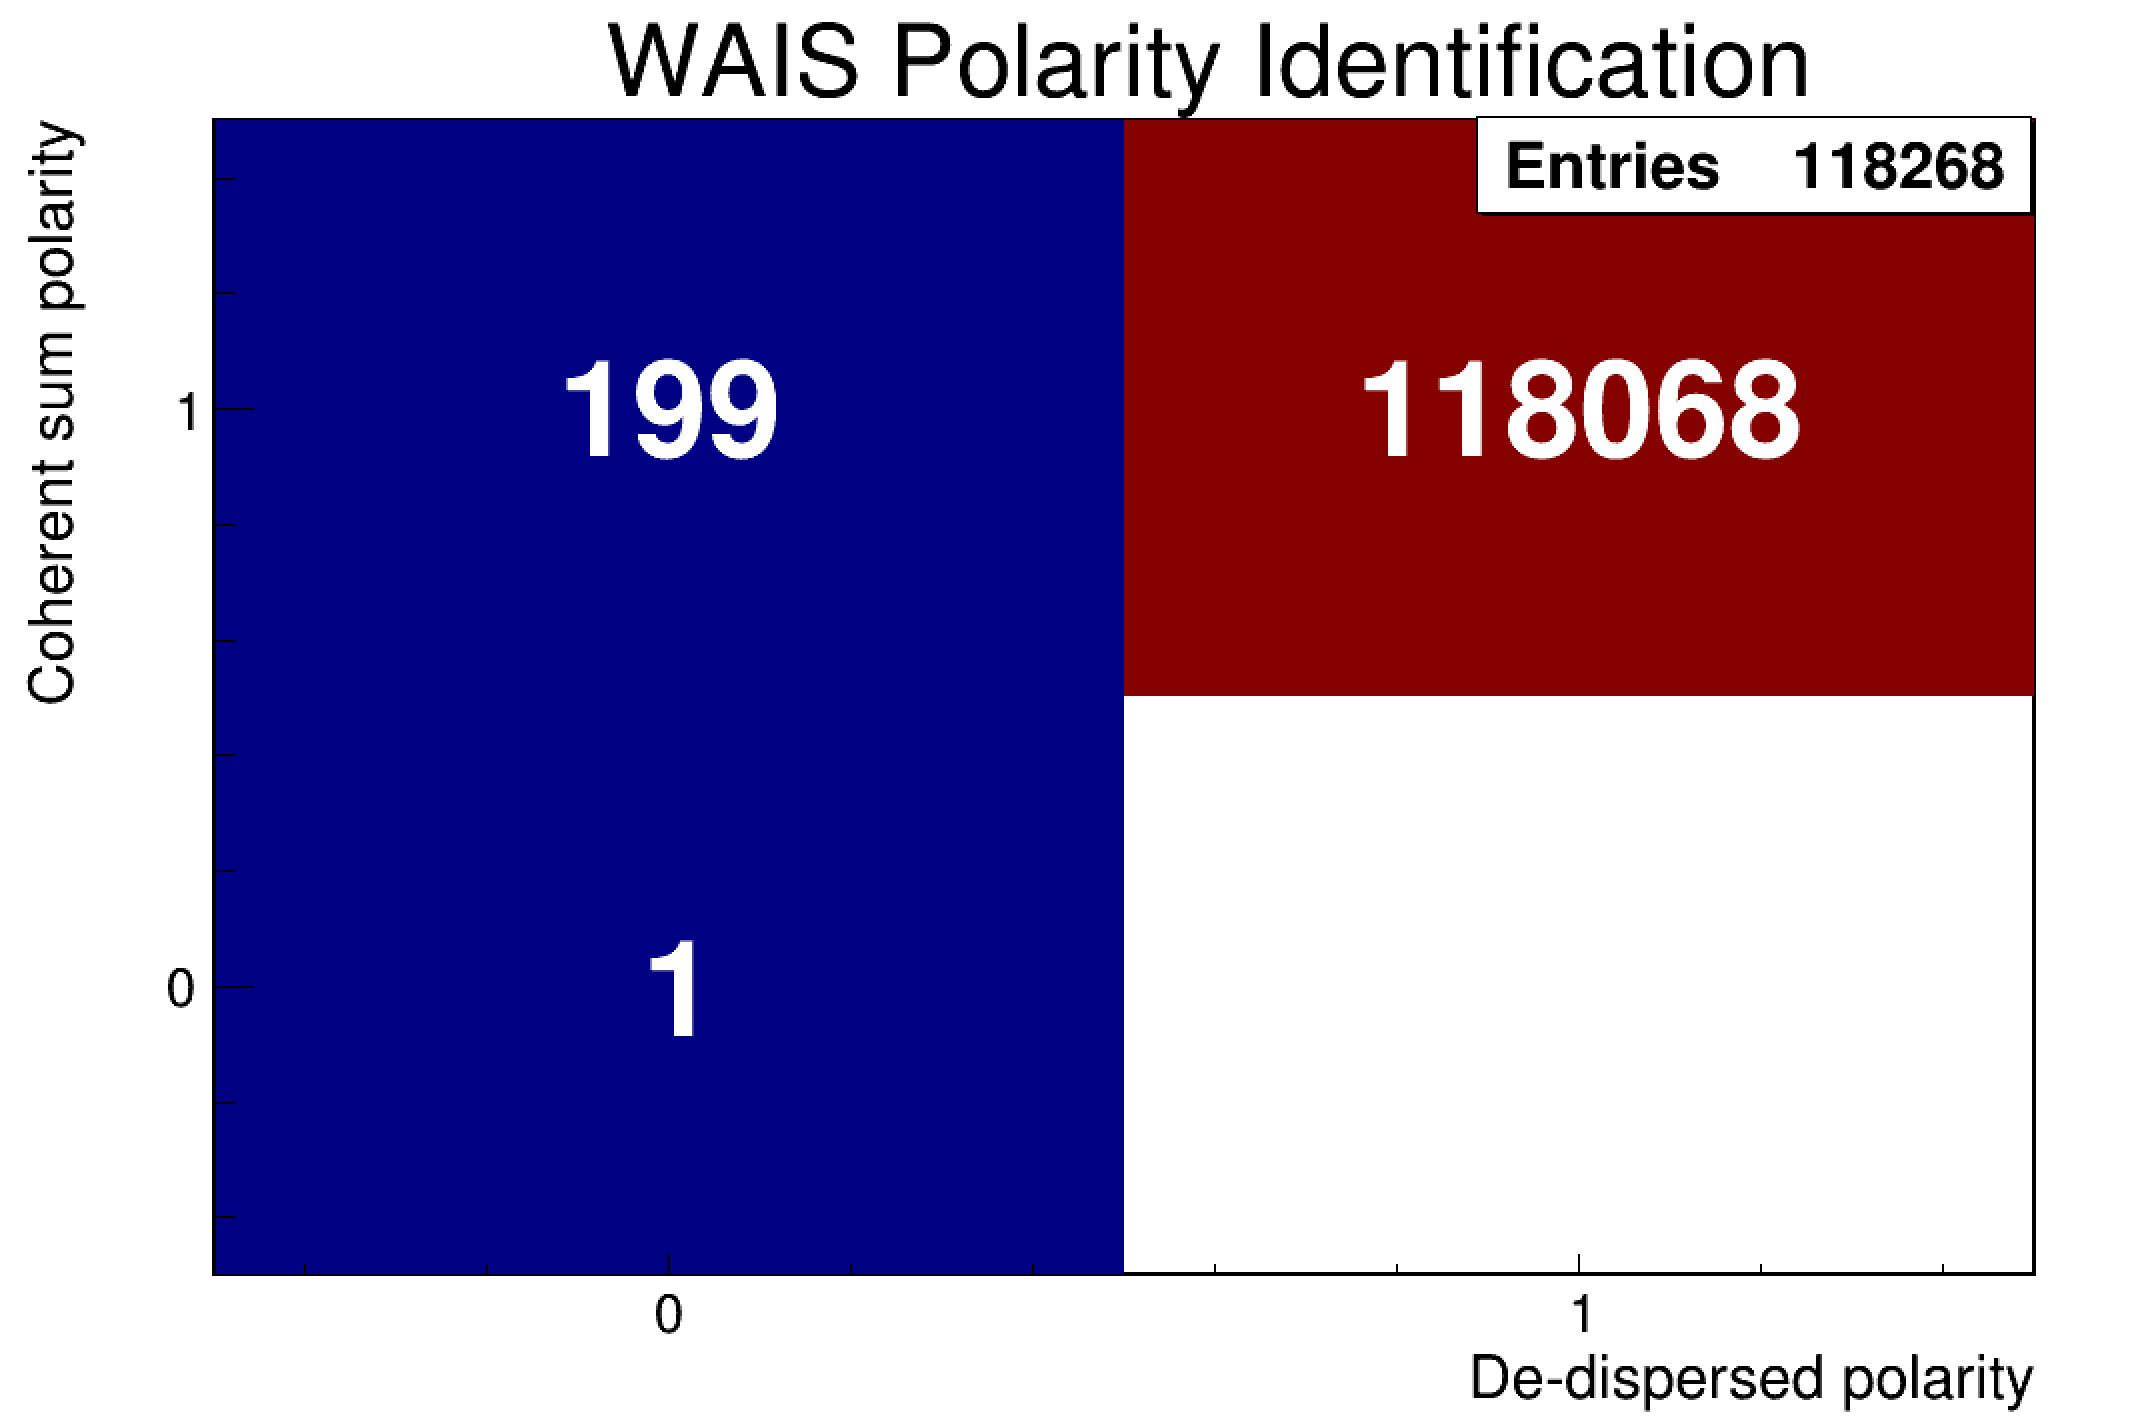
\includegraphics[width=\textwidth]{figures/waisPolarity}
	\caption{The results of the polarization identification on the 118,268 WAIS pulses.  The algorithm has a $8.46\times10^{-6}$ misidentification rate, and a $1.68\times10^{-3}$ probability of returning an indeterminate polarity.} 
	\label{fig:waisPolarity}
\end{figure}
	

		
\section{Known and Measured Source Identification}%10
	Many bases on the Antarctic continent are already cataloged by the various national programs that operate them.  Using these known bases we can eliminate events that interferometrically point to objects of expected anthropogenic noise.  There also likely exist bases that are, for whatever reason, not included in our catalog.  We also use a list of "pseudo-bases" generated from clustered event lists from previous ANITA flights to eliminate possible anthropogenic interference.  The resulting effect these excluded regions have on the flight can be determined by its flight path and a log-likelihood method for generating pointing error elipses around the bases.
	
	
	\subsection{Sun and Its Reflection, Thermal Noise Effect}
		The Sun does pass below the horizon during the austral summer, and it stays within the field of view of the ANITAIII instrument throughout the flight.  While the thermal noise from the sun is random and unpolarized in nature, it presents as a coherent noise source to the antennas where it is within their field of view.  For many events measured in the flight, the Sun presents itself as the highest interferometric peak.  However, since the sun is above an elevation angle of zero these events will not pass quality cuts. However, when the sun is at high elevation angles far from the antenna beam patter, the reflection of the sun off the ice, which is also coherent, can dominate the interferometric image.
	
	\subsection{Satellites, bases, and other ``known'' anthropogenic sources}
		The continent of Antarctica is under constant study by many scientific groups spread across the ice.  Additionally, humanity has launched orbiting artificial satellites that are equipped with radio frequency communications.  Both these sources are known to exist, and can be compiled into a list and used to mask portions of the field of view.  

	\subsection{Pseudo-bases: unknown anthropogenic sources}
		Despite the best efforts of the collaboration, it is not possible to compile a complete list of Antarctic camps during the flight to a high degree of certainty.  Because of this, it becomes necessary to use measurements from the payload itself to discern locations of human activity.  


	
\section{Event Quality Cuts}%11
	All events taken with the ANITA instrument must first pass basic checks on their ability to be considered in a sample of astrophysical impulses.  ANITAIII does not seem to suffer from significant issues related to the digitization or storage of waveforms, however there are several observed event types that can be identified and removed prior to analysis.

	\subsection{RF Triggered}
		The first requirement for an impulse to be considered as a CR candidate is that the RF trigger must have initiated the readout.  The 2Hz of minimum bias triggers are therefore excluded from the analysis.

	\subsection{Calibration Pulsers}
		Accurate tagging of calibration pulsers allows us to remove them from the sample considered in the physics analysis.  This is done using the recorded nanosecond precision trigger time, a knowledge of the time in each second where each pulser fired, and the time of flight between the payload at the event record time and the calibration pusler.  These events are known, do not contribute to either the background or can be considered as signal, and are thus removed.

	\subsection{Payload Blasts}
		The ANITAIII flight was plagued by high power signals that seem to emanate from the payload.  These events, called payload blasts, have a large amplitude signal in several neighboring phi sectors and tend to happen in rapid succession.  A sample payload blast event can be seen in Figure \ref{fig:payloadBlast}.  The blasts characteristically have high total RF power in the bottom two rings of antennas, but very little signal power in the top ring, suggesting that these events have a source on-board the payload.  Blasts also do not have high interferometric peaks, adding further evidence that they are spherically propagating electromagnetic waves with a source on the payload, and suggesting that they will likely be removed through signal cuts later in the analysis process.
		
		The primary metric used to select and remove these events is this ratio of total waveform power between top and bottom rings (Equation \ref{eqn:topToBottom}). This distribution can be seen in Figure \ref{fig:payloadBlastDist}.  The cut for these events was placed at a value of 3, which eliminates approximately 731k  events (1.77\%) of events from the Hpol data set, while effecting a trivial number of non-RF triggered thermal events.  The source of these blasts is unknown, though there is much speculation to their cause, and were present in both the ANITAI and ANITAII flights.  Removing these events from the dataset is done prior to all other analysis steps.  
		
\begin{equation}
	R_{topToBottom} = \cfrac{\sum\limits_{n=0}^{N} V^{2}_{bottom}}{\sum\limits_{n=0}^{N} V^{2}_{top}}
	\label{eqn:topToBottom}
\end{equation}
		
\begin{figure}
	\centering
	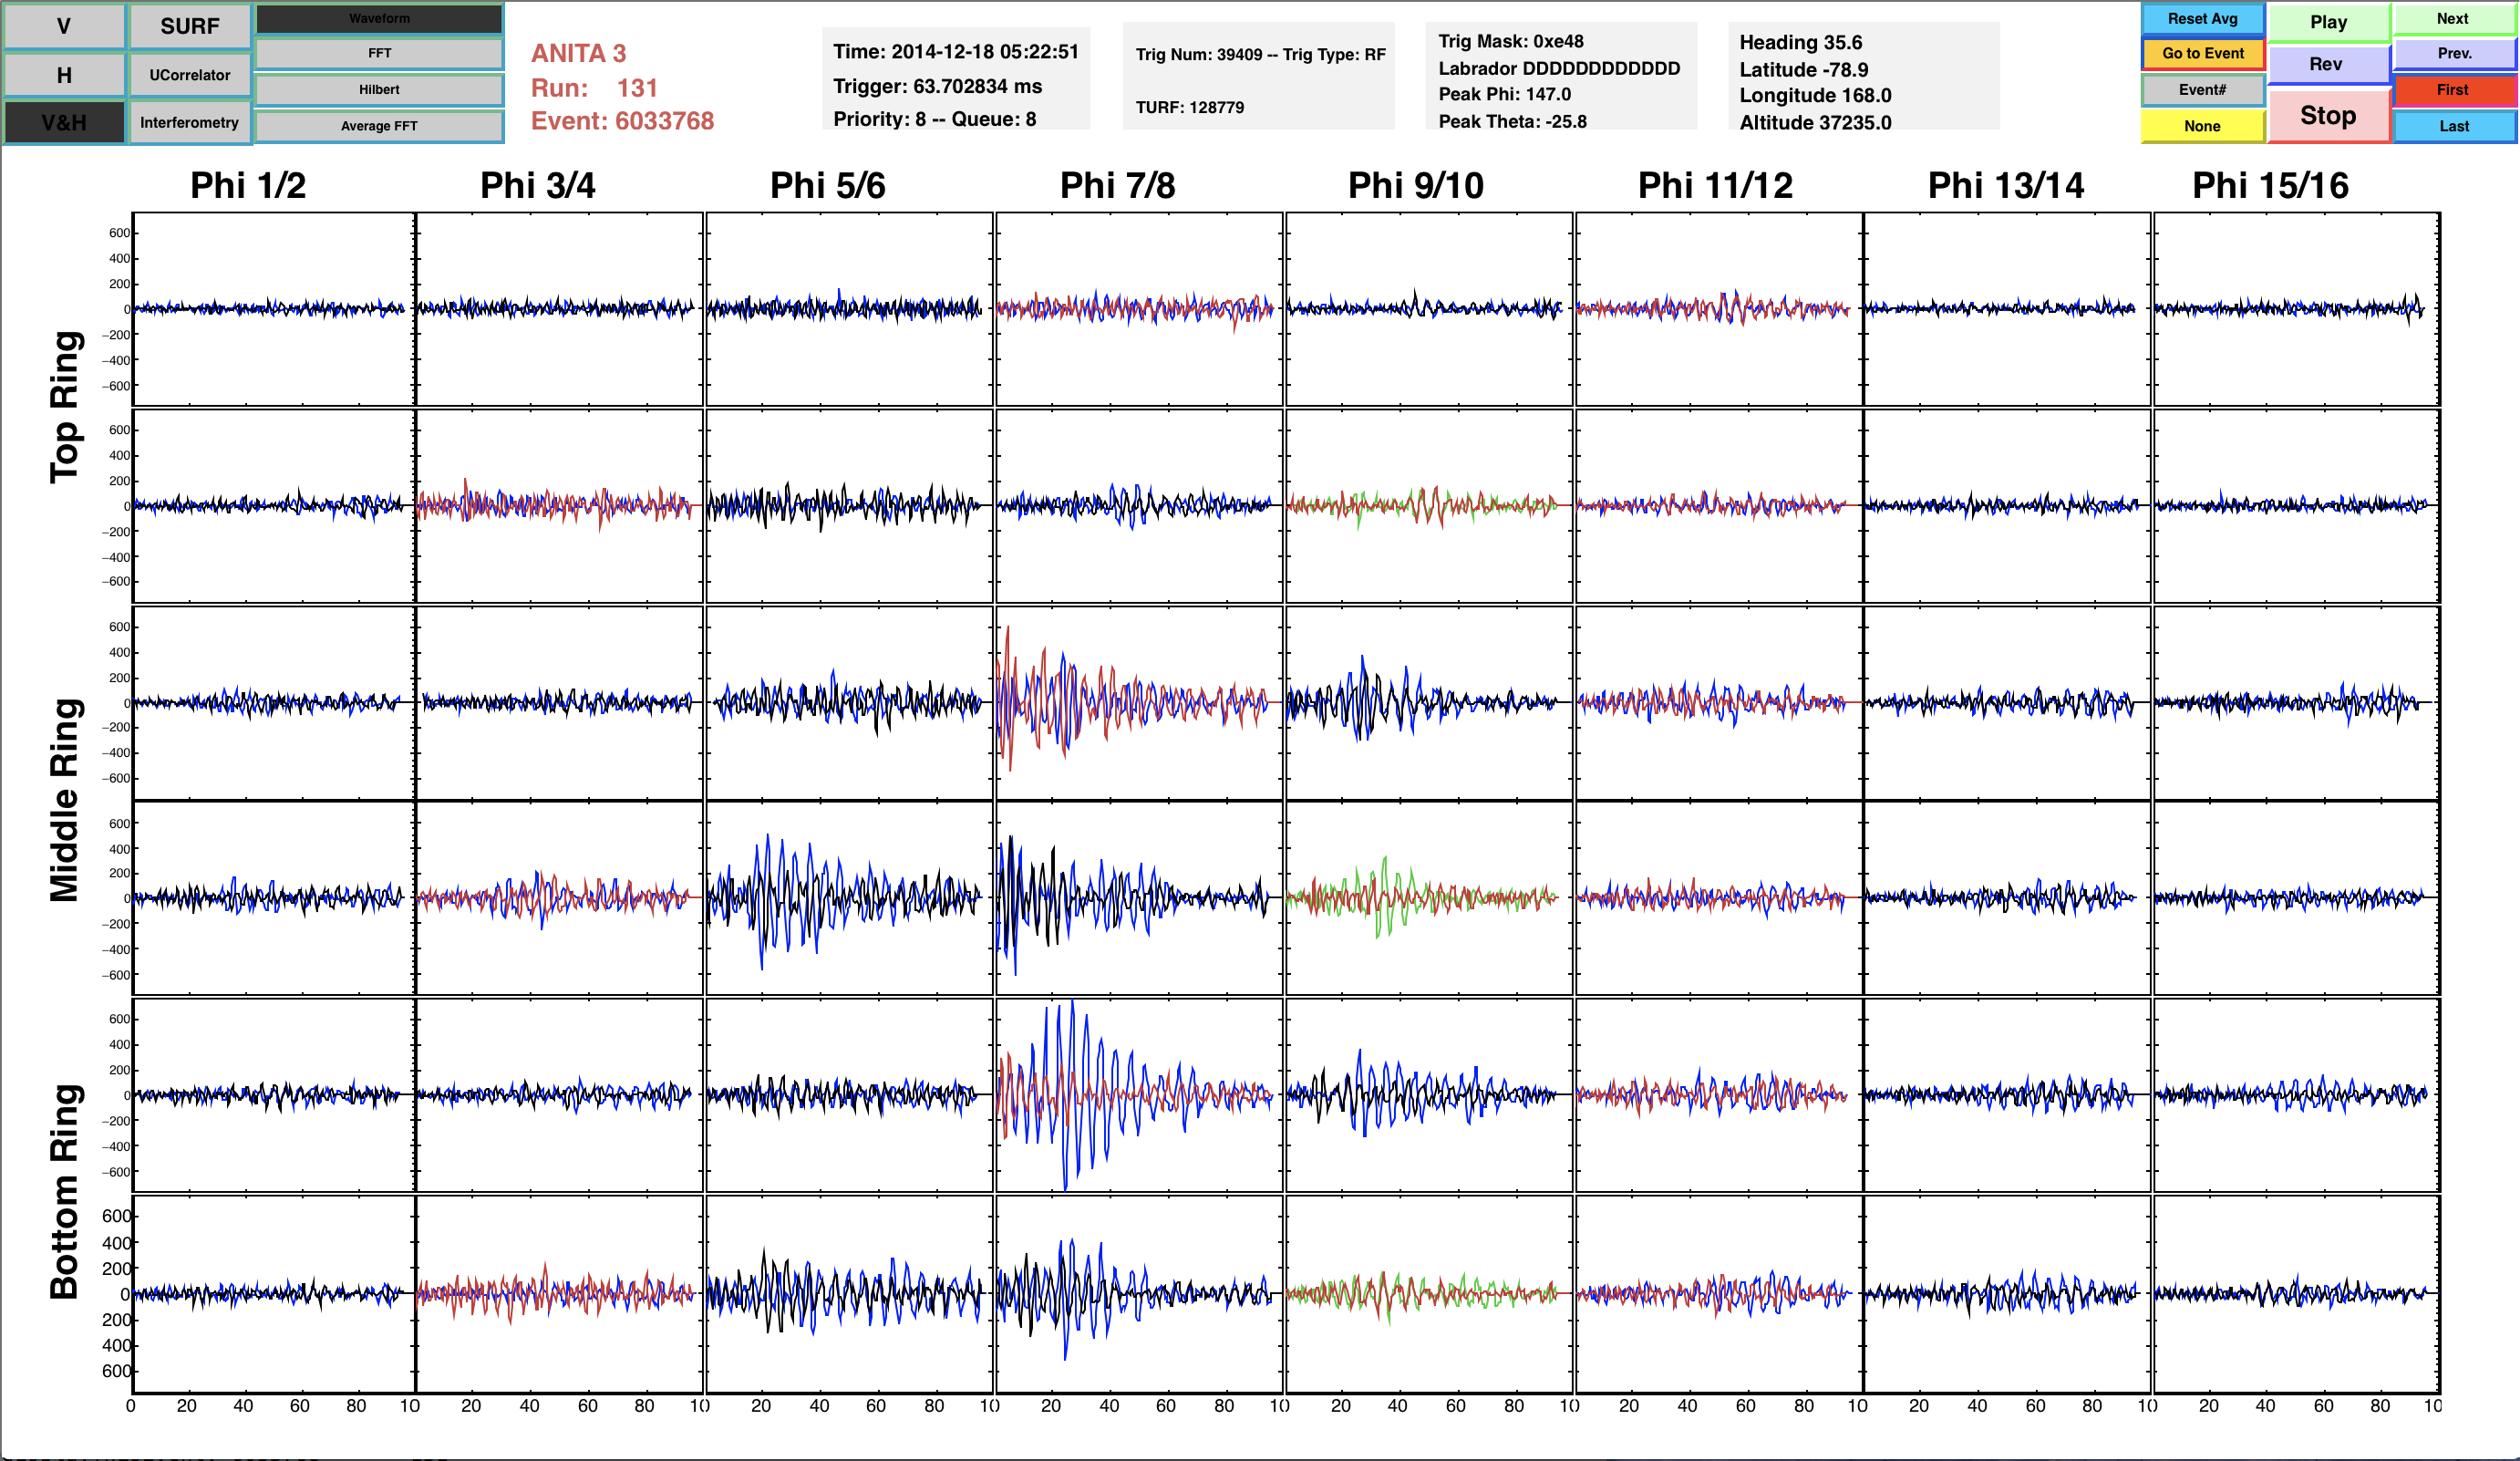
\includegraphics[height=0.5\textheight]{figures/payloadBlast}
	\caption{A magicDisplay screen capture of a suspected payload blast event.  This event was selected due to the high ratio of power between the top and bottom antenna, 6.15 for this particular event.  This pulse is additionally part of a 14 event train of pulses}
	\label{fig:payloadBlast}
\end{figure}

\begin{figure}
	\centering
	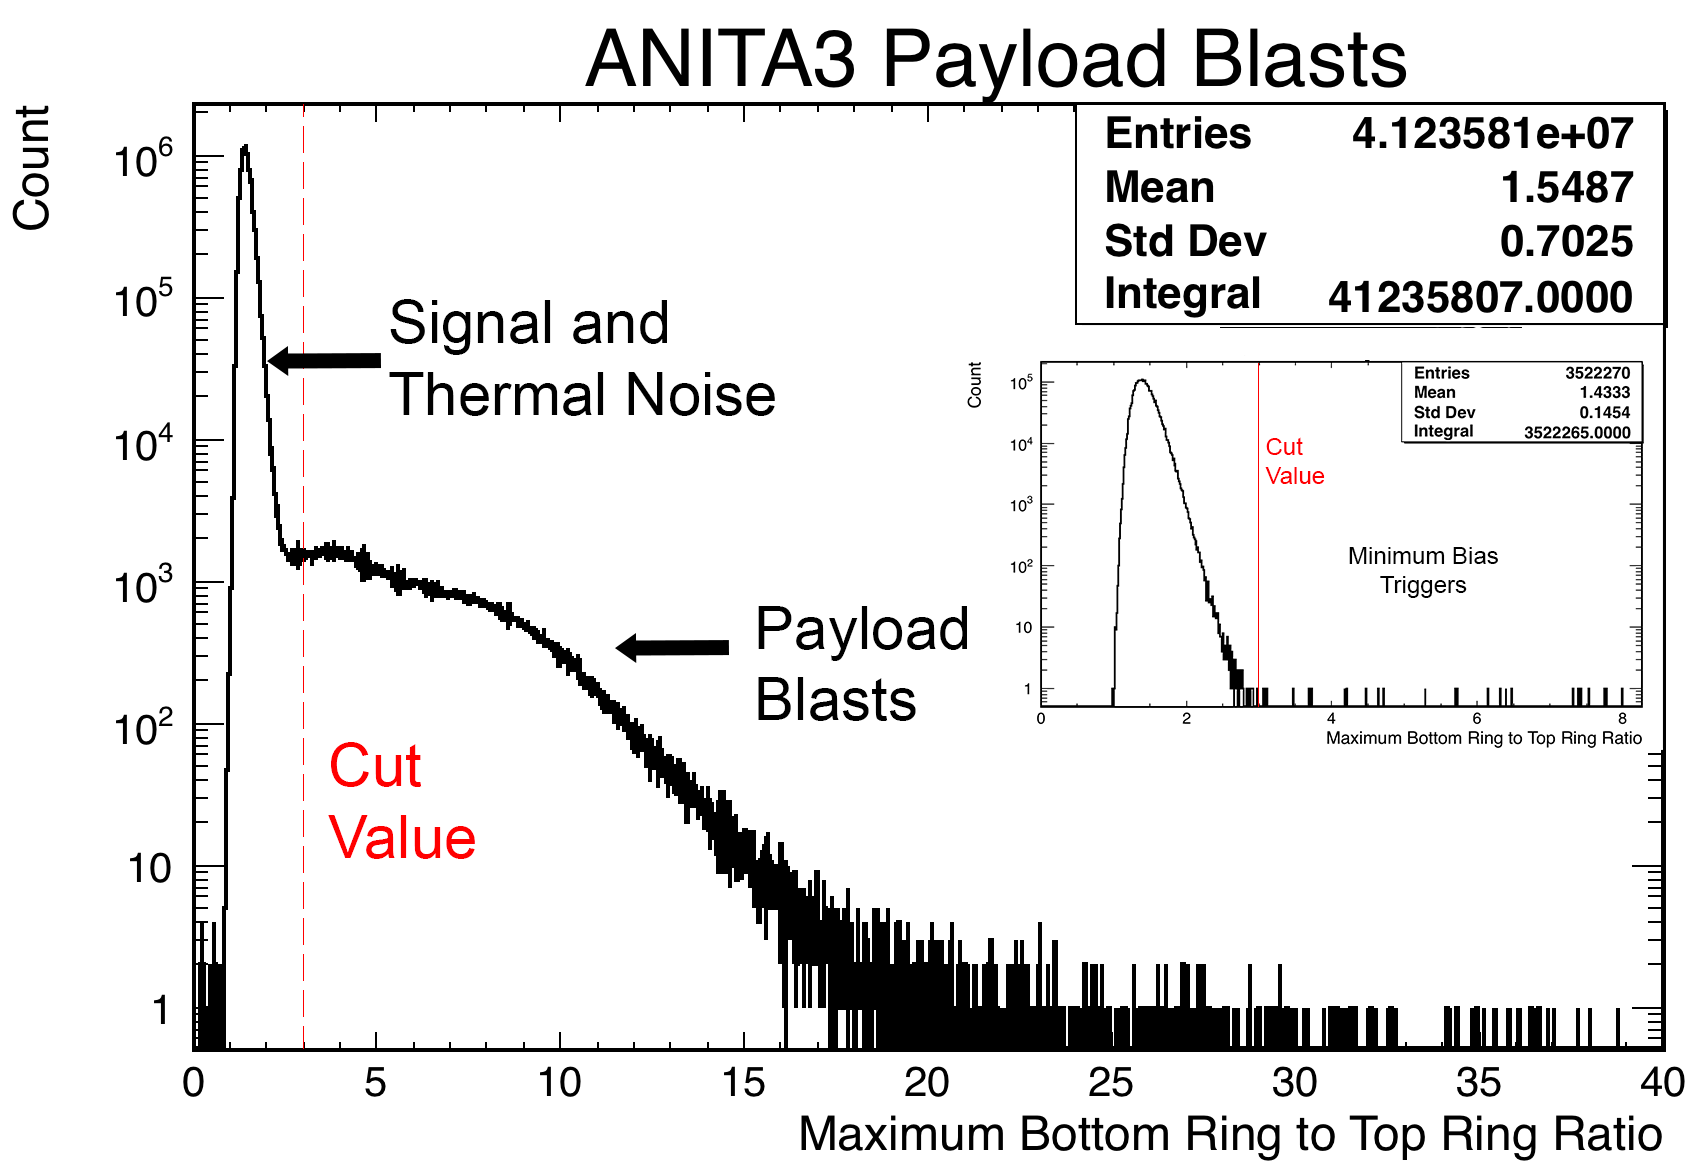
\includegraphics[height=0.5\textheight]{figures/payloadBlastDistribution}
	\caption{The event distribution of the ratio between the power measured in top and bottom rings of antenna for all horizontal polarization triggered phi sectors.  The distribution for non-RF triggered events is displayed as well, within the full distribution plot.  Red dashed lines denote the location of the quality cut.}
	\label{fig:payloadBlastDist}
\end{figure}
	
%	\subsection{SURF Saturation}
%		A small fraction of events have recorded voltage values outside the dynamic range of the LABRADOR digitizer.  Though several of these are from extremely high power sources within the field of view, several saturation events are caused by single bit errors in LABRADOR digitization.  These have the characteristic of having a single voltage sample with a value a power of two higher than the remaining points in a waveform.  For simplicity, all events with these bit errors are excluded.
		
		
	\subsection{Downward pointing, above horizontal events}
		Events that have an interferometric map peak that points upwards cannot be created by any of the astrophysical event types under consideration for this analysis.  ANITAIII floats at the top of the stratosphere, above which there is sparingly small amounts of atmosphere with which a particle can interact.  Even direct CRs will have impulsive signals that emanate from within the atmosphere.  Because of this, all events that have peak elevation angles above zero can be safely discarded.
		
	
	\subsection{Delayed waveforms: reconstructed angle to hardware trigger angle cut}
		The dynamic phi sector masking introduces a class of events in which the waveform ``falls off'' the end of the digitization record, subsequently losing information about the earliest structure in the waveform.  This is caused when impulsive events hit the payload in a masked phi sector, but have a sufficient amount of power to trigger channels with antennas in un-masked phi sectors, despite the large angles from their peak gain boresight.  The majority of the signal power will still be observed in channels pointing towards the impulsive source, however the free space propagation time between the masked and unmasked phi sectors delay the trigger formation enough so that the waveform is truncated and information is lost.  An example of this non-ideality can be seen in Figure \ref{fig:earlyWaveform}.
		
		Since these waveforms are missing important information, and the incident electric field cannot be reliably reconstructed, they can not be included in a final signal sample.  To ensure that the at least one antenna involved with the coherent sum is included in the reported hardware trigger, this cut is set at $45^\circ$.
		
\begin{figure}
	\centering
	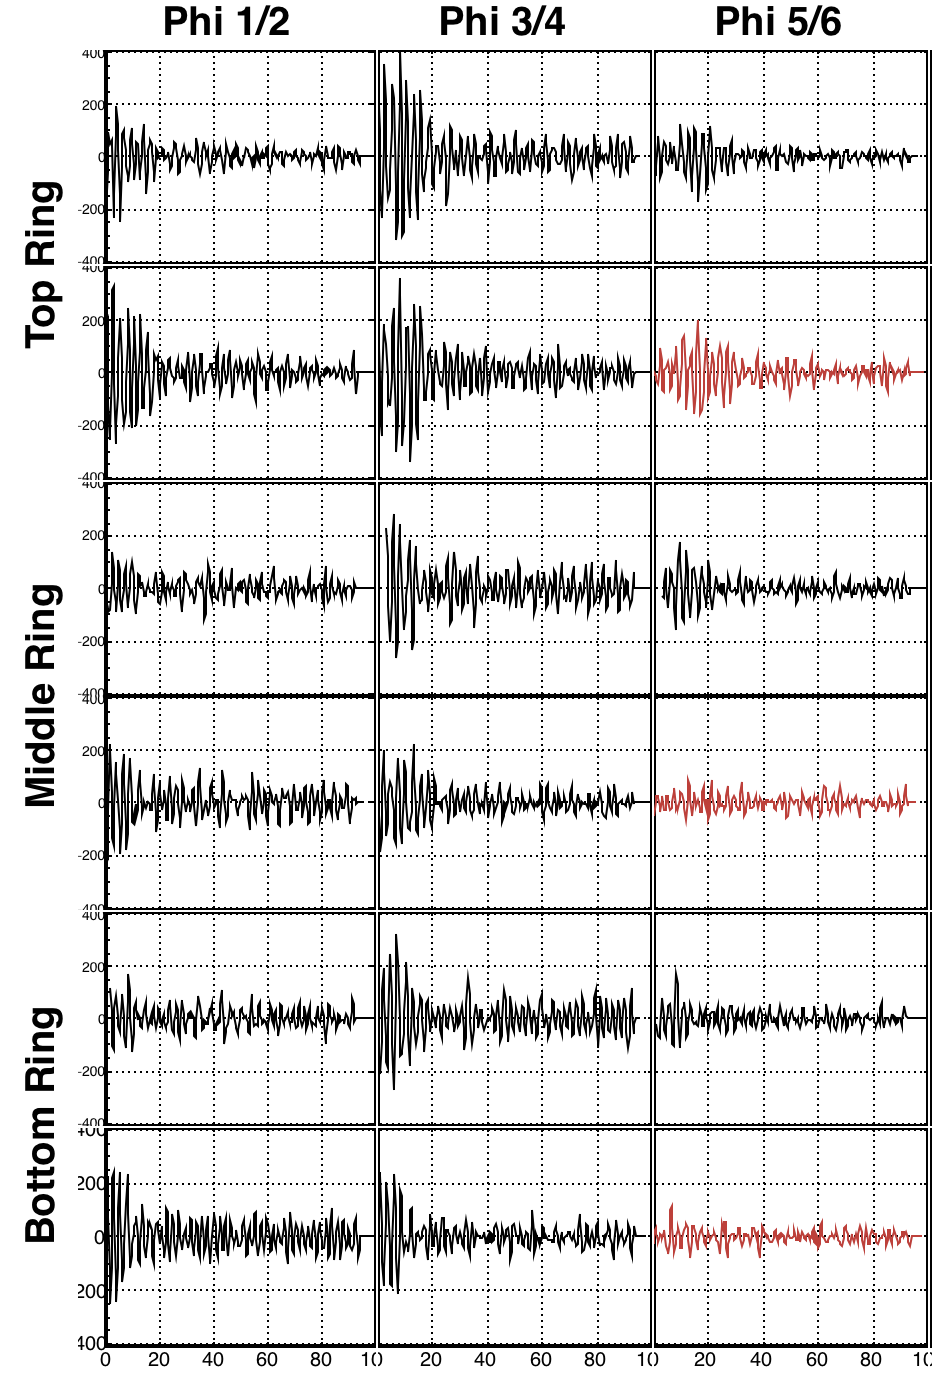
\includegraphics[height=0.85\textheight]{figures/EarlyWaveform}
	\caption{An example of a waveform where the promptest radiative component has fallen off the record and is not recorded.  The red waveforms note channels which were reported to be involved in the trigger by the hardware.  This event, 5877965, has a difference between the peak map angle and the hardware trigger angle of $77.5^\circ$.} 
	\label{fig:earlyWaveform}
\end{figure}		


		
	\subsection{Major Bases}
		WAIS Divide and McMurdo Station are, for this analysis, defined as major bases which are removed prior to analysis.  These bases have some of the highest activity on the continent, and the sheer number of events that come from these two bases has the effect of biasing the remainder of the analysis.  Any event that reconstructs near either base is excluded.  Nearness is conservatively defined as the map peak being within a geometric angular sum of 6$^circ$ of the geographic coordinates of either base.  This check is only done if the payload is within 700km of either base.  This cut will also exclude any calibration pulsers from either base that are not correctly tagged.


	\subsection{Effect of quality cuts on number of events}
		The quality cuts remove a large fraction of the events recorded by the payload.  The number removed by each cut can be found in Table \ref{tab:qualityCutReason}.  The resulting quality cut event list contains 2,670,191 events. %REVISE
		
		\begin{figure}
		\centering
		\begin{tabular}[c]{|l|c|c|c|}
		\hline
		Cut Parameter & Events Failed  \\
		 & (Single)  \\
		\hline
		LDB Pulser & 342,108 \\
		WAIS Pulser & 118,458 \\
		Points to LDB* & 314,438 \\
		Points to WAIS* & 17,188 \\
		Above Horizontal & 10,106,687 \\
		Hardware Trigger Angle & 28,022,208 \\
		Payload Blast & 733,458 \\
		Not RF Triggered & 3,571,726 \\
		\hline
		\end{tabular}
		\caption{The number of events removed by each quality cut from the set of events with H-pol triggers.  The cuts remove any event with a single value below those in Table \ref{tab:cutValues}.  Events that are removed by several cuts are double counted, unless denoted by a ``*'', when tagged calibration pulser events are removed prior to determining removed event quantities.}
		\label{tab:qualityCutReason}
		\end{figure}



\section{Analysis Cut Methodology}%12
	Cut values that separate astrophysical sources from thermal and non-astrophysical anthropogenic background are determined by examining the distributions of various cut parameters for triggered events.  The most desirable cut value will be one that maximizes the quantity CR-like while minimizing the number of thermal or anthropogenically triggered events.
	
	First, distributions of values for events that point at known major Antarctic bases are examined to determine a level which would capture weaker bases to high likelihood in order to identify and exclude them.    This first more general ``impulsivity'' cut will capture information about locations on the continent that produce impulsive signal distributions that may leak into the signal. This allows clustering to remove generators of impulsive signals.
	
	Secondly, WAIS calibration pulses were examined as a representative signal source.  In order to extract the highest number of events with measured quantities most similar to an expected CR EAS radiation pattern, cuts were selected primarily to maximize efficiency on signal, and allow for a maximum exposure for the analysis.  An a posteriori background estimate (discussed later in \autoref{sec:backgroundEstimate}) that examines the underlying localized distributions of events will be performed on all CR candidates in order to further constrain and quantify the background that leaks into the signal region.
	
	Six calculated values were considered for the cuts.  These are: the peak of the interferometric map (map peak), the peak of the Hilbert envelope of the coherently summed waveform (hilbert peak), the linear polarization fraction of the coherently summed waveform, and the template correlation peak value for both the coherently summed and for the de-dispersed waveforms.  These values, whose calculations are described above, require that the measured signals both are impulsive and have a shape comparable to a CR.  Plots of these values for the non-RF triggered events, for events that point at major bases, and for the WAIS pulses are shown in Figures \ref{fig:mapPeakCut}, \ref{fig:hilbertCut}, \ref{fig:linPolCut}, \ref{fig:templateCoherCut}, and \ref{fig:templateDeconvCut}.  As a note, the template used for the analysis of WAIS pulses was the coherently summed and averaged WAIS pulse, derived from measurements.
	
	
\begin{figure}
	\centering
	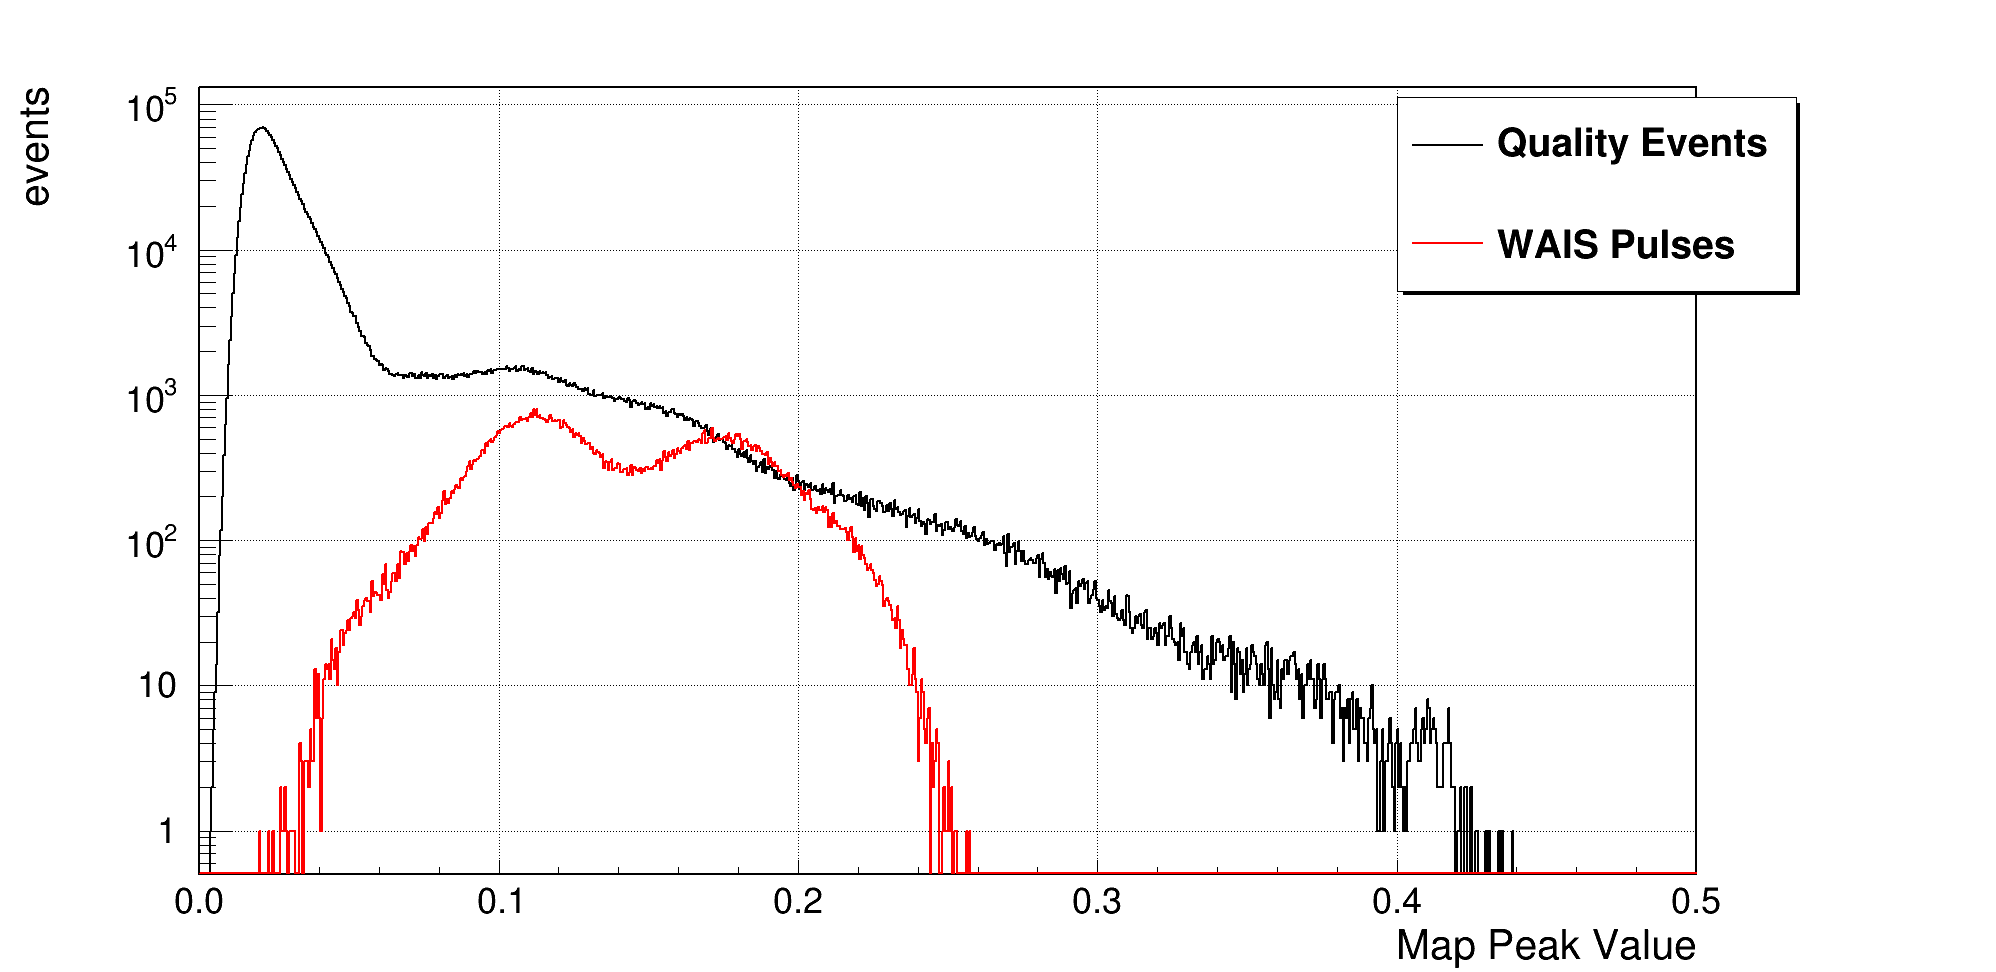
\includegraphics[width=\textwidth]{figures/mapPeakCut}
	\caption{Distribution of interferometric map peak values for events that pass quality cuts and WAIS calibration pulser events.} 
	\label{fig:mapPeakCut}
\end{figure}
	
\begin{figure}
	\centering
	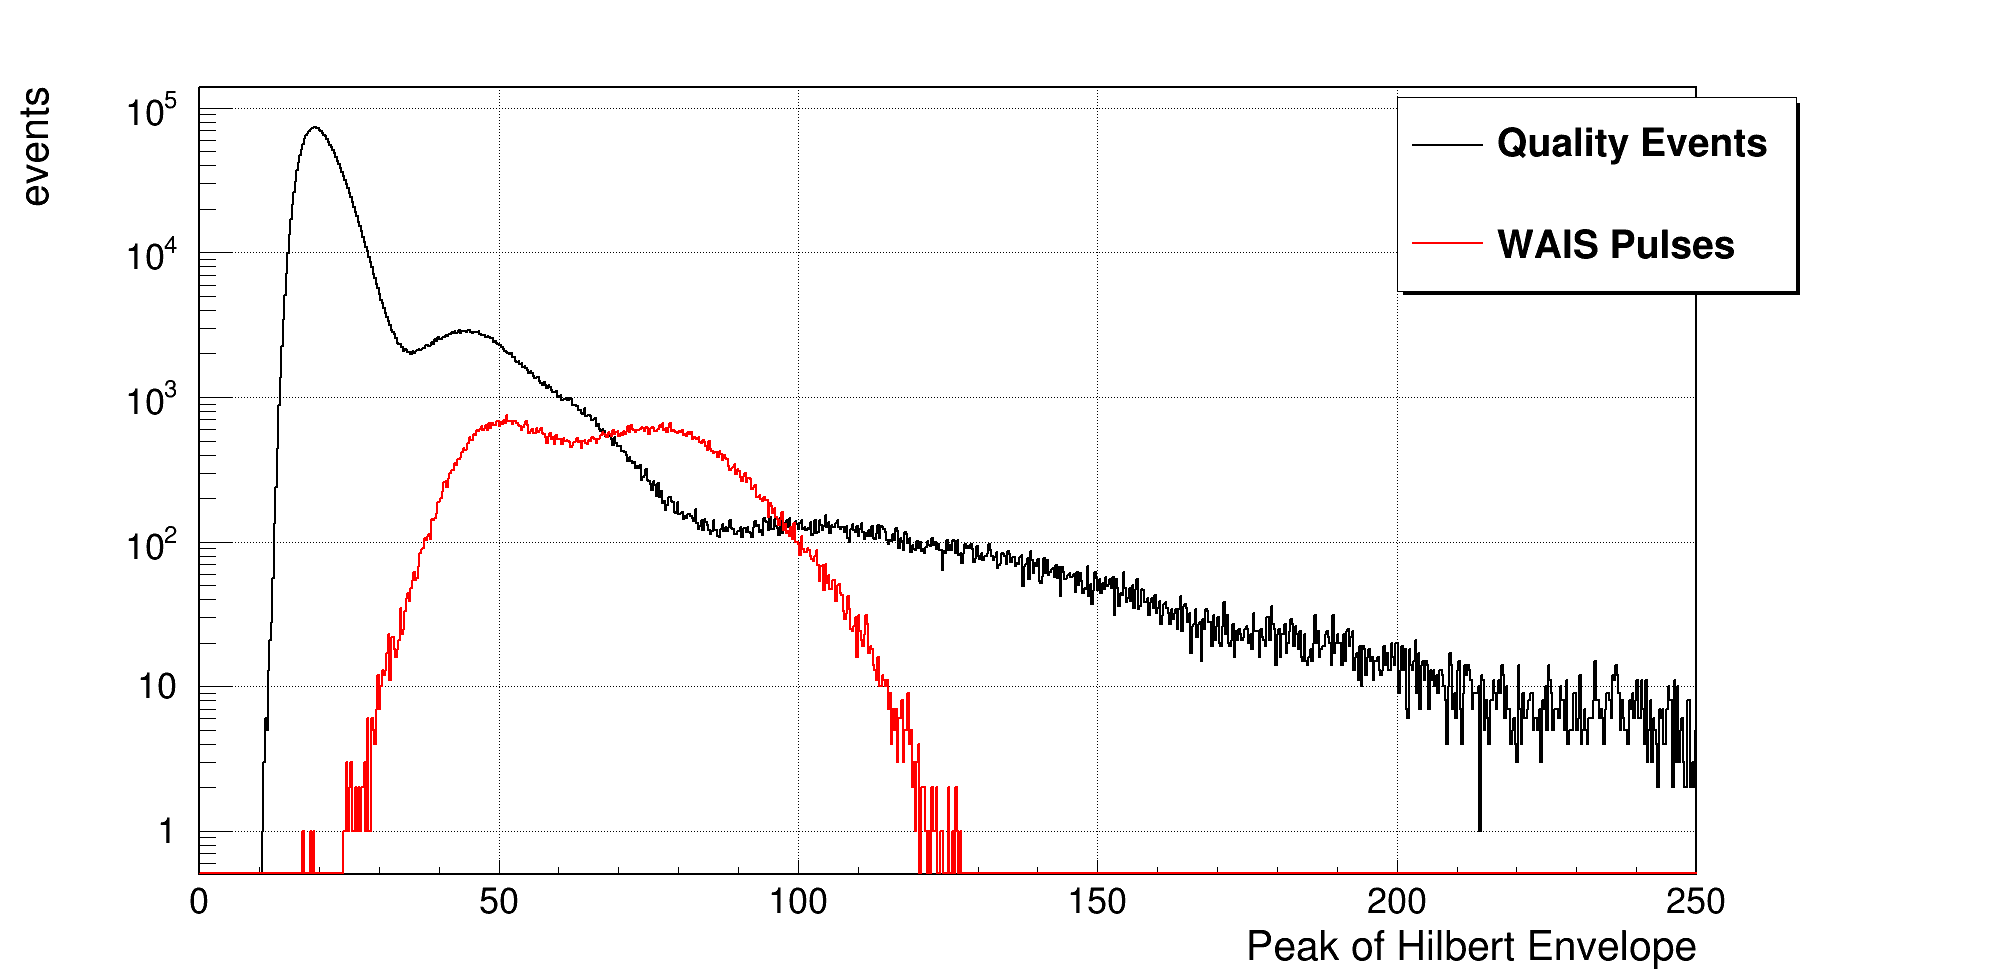
\includegraphics[width=\textwidth]{figures/hilbertCut}
	\caption{Distribution of Hilbert envelope peak values for events that pass quality cuts and WAIS calibration pulser events.} 
	\label{fig:hilbertCut}
\end{figure}

\begin{figure}
	\centering
	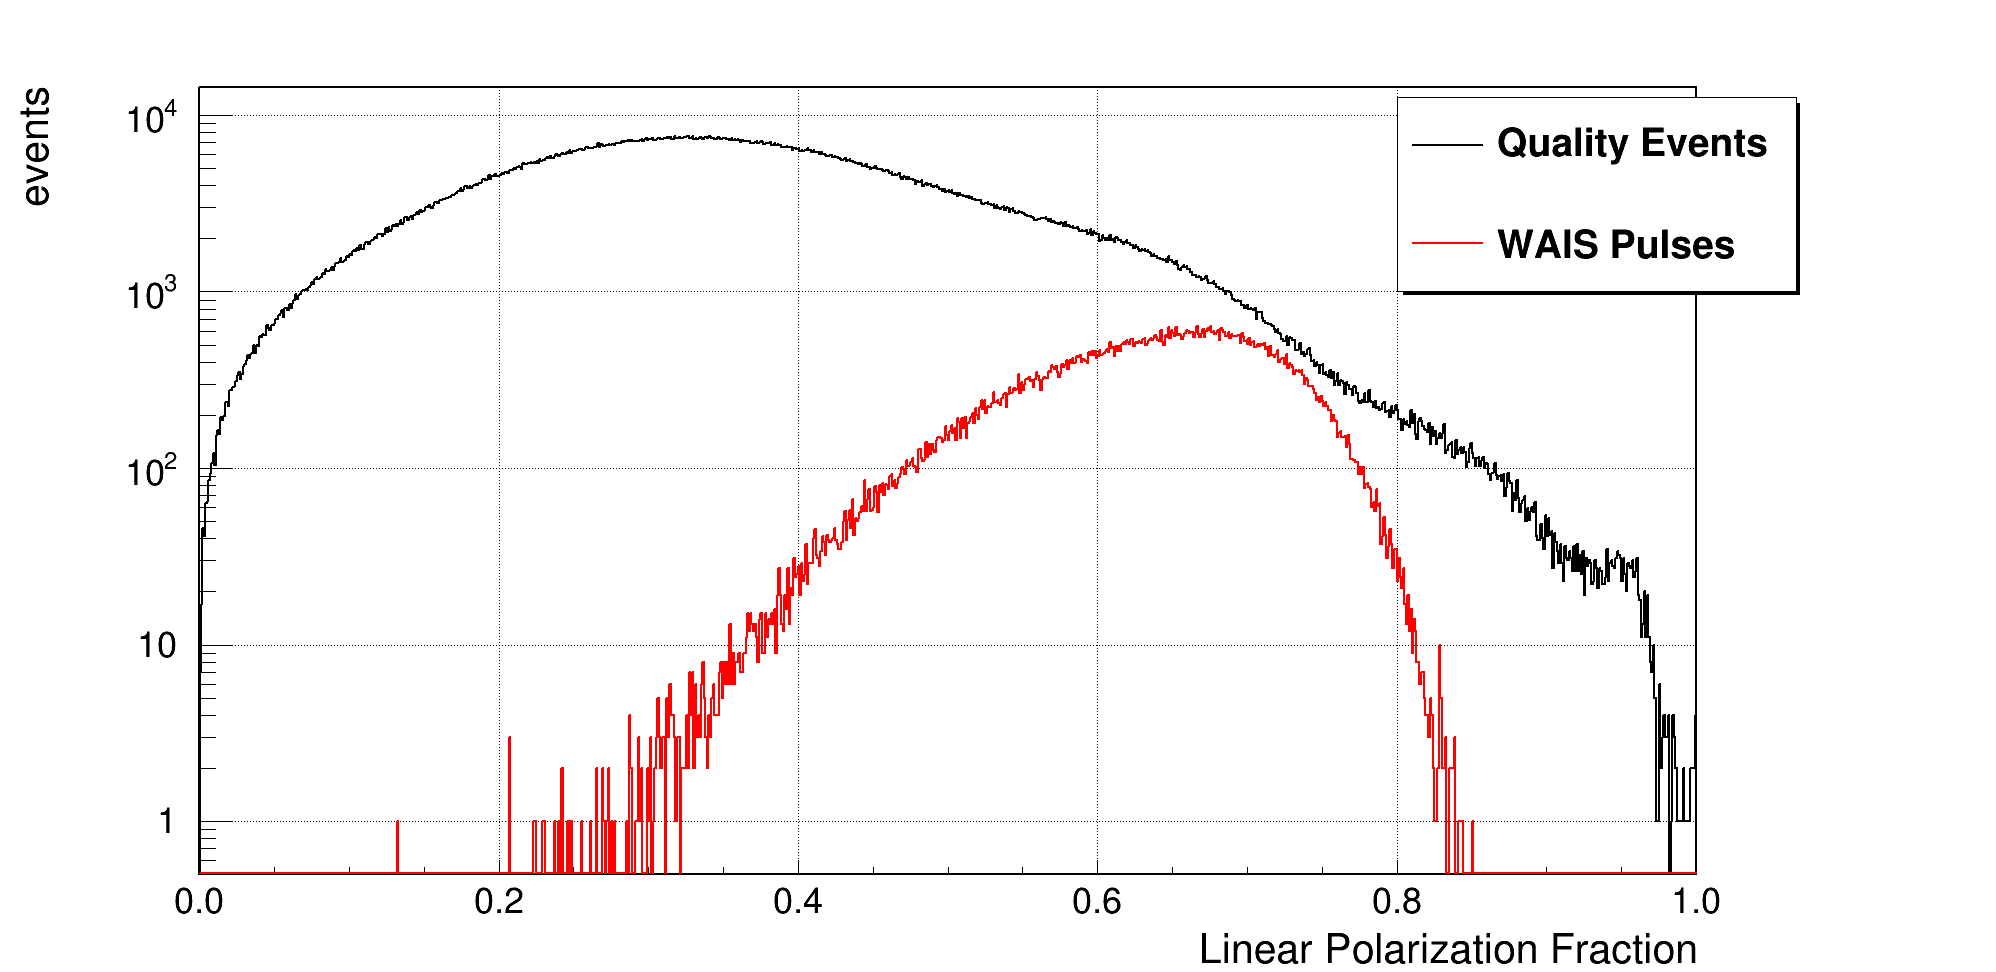
\includegraphics[width=\textwidth]{figures/linPolCut}
	\caption{Distribution of linear polarization fractions for events that pass quality cuts and WAIS calibration pulser events.} 
	\label{fig:linPolCut}
\end{figure}

\begin{figure}
	\centering
	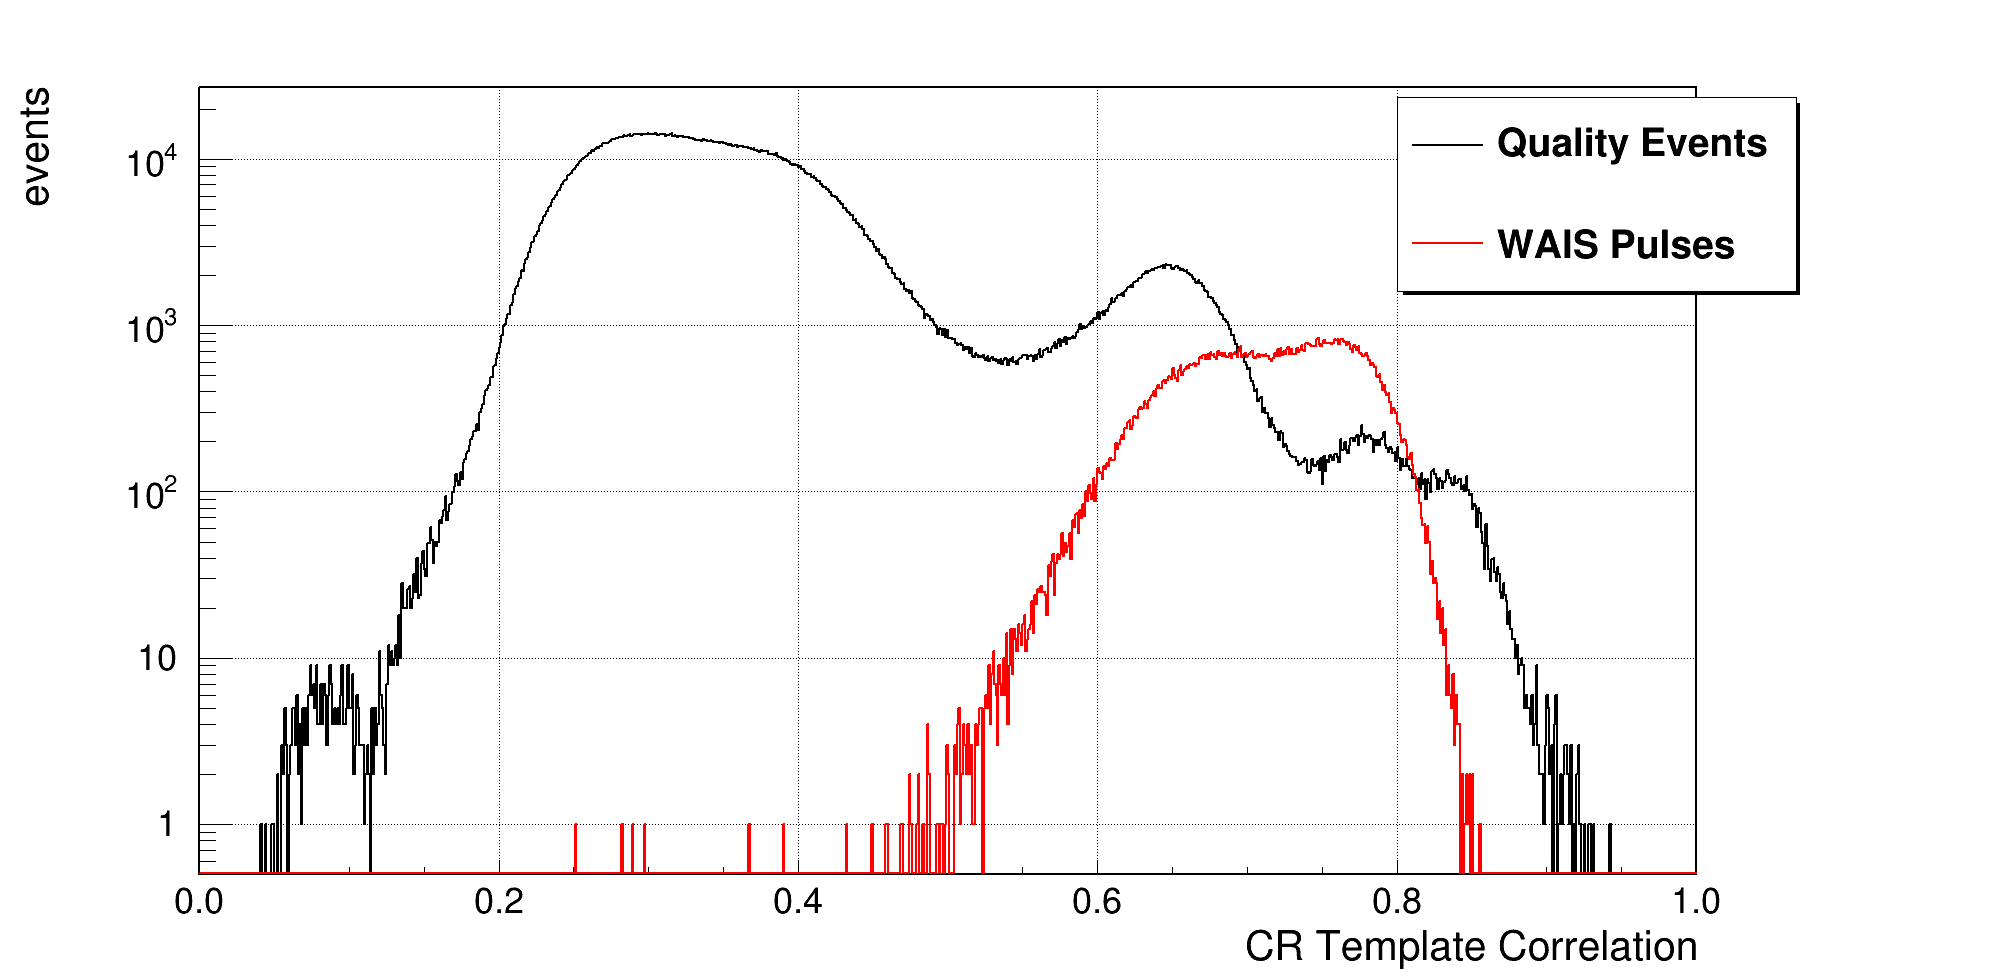
\includegraphics[width=\textwidth]{figures/tempCorrCut}
	\caption{Distribution of peak cosmic ray template correlation values for events that pass quality cuts and WAIS calibration pulser events.} 
	\label{fig:templateCoherCut}
\end{figure}

\begin{figure}
	\centering
%	\includegraphics[width=\textwidth]{figures/tempDeconvCut}
	\caption{Distribution of peak cosmic ray template correlation values for events that pass quality cuts and WAIS calibration pulser events.} 
	\label{fig:tempDeconvCut}
\end{figure}
	
	
The values for the cuts are shown in Table \ref{tab:cutValues}.  The final signal cut values were set so that 99.9\% of WAIS pulser events are captured.

\begin{figure}
\begin{tabular}[c]{|l|c|c|}
\hline
Quantity Name & Impulsivity Cut Value & Signal Cut Value \\
\hline
Map Peak & 0.0435 & 0.0435 \\
Map SNR & 9.05 & 9.05 \\
Hilbert Peak & 25.0 & 31.1 \\
Linear Polarization Fraction & 0.50 & 0.60 \\
Coherent Template Correlation & 0.50 & 0.666 \\
Deconvolved Tempalte Correlation & 0.50 & 0.666 \\
\hline
\end{tabular}
\caption{Values used for impulsivity and signal cuts.  Impulsivity cuts are derived from measurements of known major bases, which produce a wide range of anthropogenic signals.  Signal cuts were determined from WAIS pulser measurements.  Determinations of the cuts is detailed in the text.}
\label{tab:cutValues}
\end{figure}



\section{Geographic Clustering}%13
	After enriching the event sample by removing events with a high probability of being thermal noise or non-impulsive anthropogenic background, geographical clustering of the events can be done to further discriminate against backgrounds. Astrophysical signal events are expected to be isotropically distributed evenly across the continent, as there is no preferred cardinal direction for UHECR or UHE$\nu_{\tau}$ detections.  Human activity, on the other hand, tends to cluster around regions of logistical or scientific interest.  Anthropogenic background sources are thus expected to point at other captured events, which can be used to discriminate against them and further refine the data sample.

	\subsection{Base Clustering}
		Through communication with various international Antarctic institutions, a list of active camps and other human activity on the continent was compiled for the time frame of the ANITAIII flight.  An image of these bases mapped to the continent can be seen in Figure \ref{fig:BaseMap}.  However these bases are not used to exclude any signal events.  Determining the validity of this base map is plagued with issues, as they are run an managed by a large collection of different nations and groups, many of whom do not wish or care to make their activities publicly available.  Additionally, camps that are reported by groups may be inactive, or have moved from when they were last reported.  Due to this non-statistical and very difficult to model uncertainty, the relationship between any impulsive event and a camp present on the list does not significantly enhance our understanding of the source of such event.  We must therefore employ alternate means to estimate the likelihood that a specific event is anthropogenic or astrophysical in nature.
		
\begin{figure}
	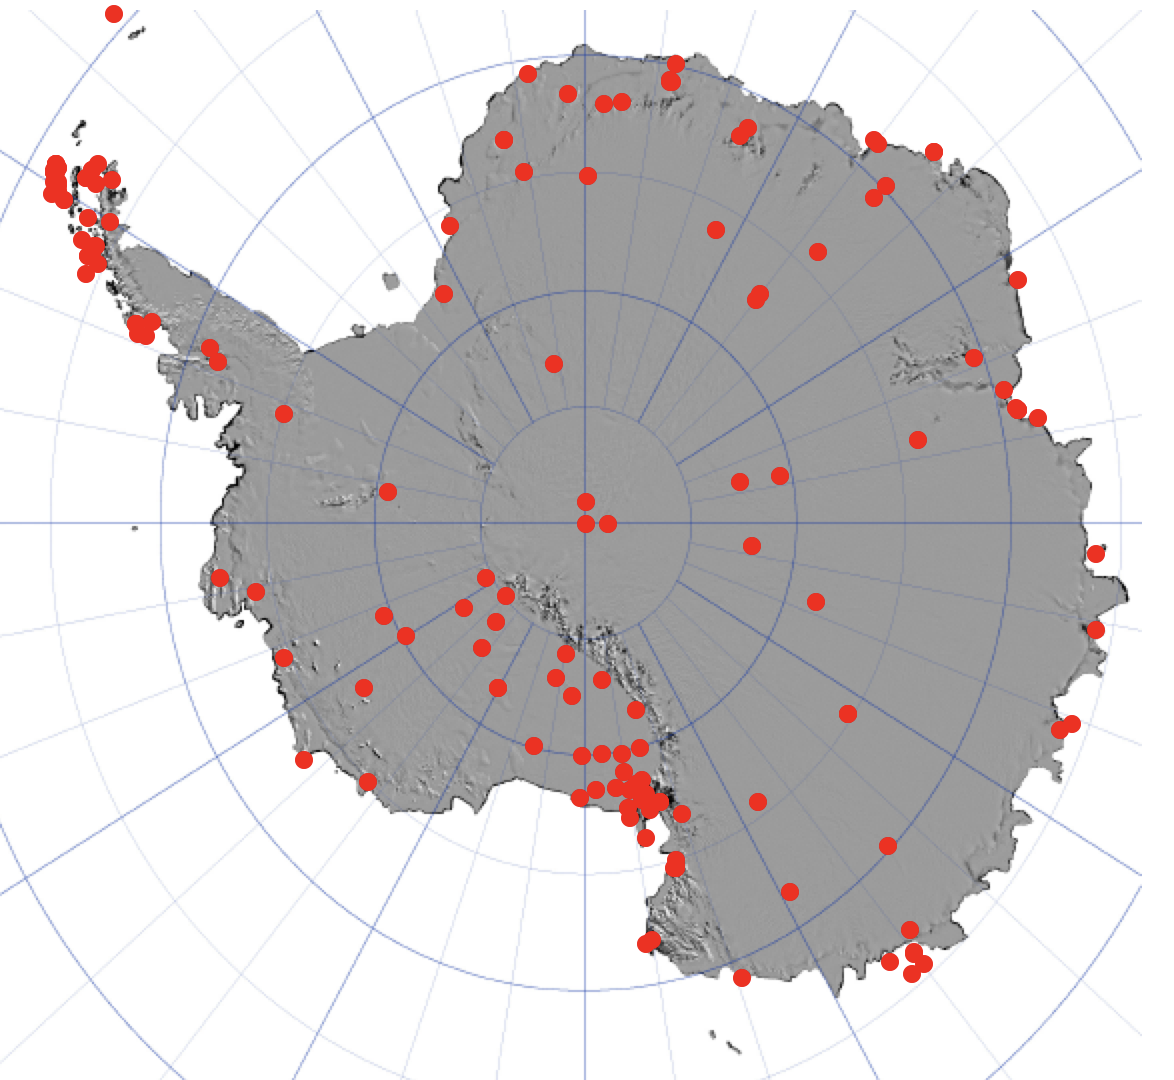
\includegraphics[width=\textwidth]{figures/BaseMap}
	\caption{A map of the recorded human activity on the continent of Antarctica during the ANITAIII flight.}
	\label{fig:BaseMap}
\end{figure}	
	
	
	\subsection{Log likelihood clustering metric}
		Impulsive events that point back to a geographically isolated source location have the highest likelihood to be astrophysical in nature.  The metric that has been used in past ANITA experiments to determine the ``closeness'' of one event to another has been called the Log Likelihood, and is represented by the variable $L$.  This measurement must take into account both the pointing uncertainty of the instrument, as well as the constantly changing payload location.  Since each event can be seen from a different angle, the angular separation between the projected location of one event on the ice from the perspective of another event may not be the same as the inverse.  This is shown graphically in Figure \ref{fig:clusteringProjection}.  

\begin{figure}
	\centering
	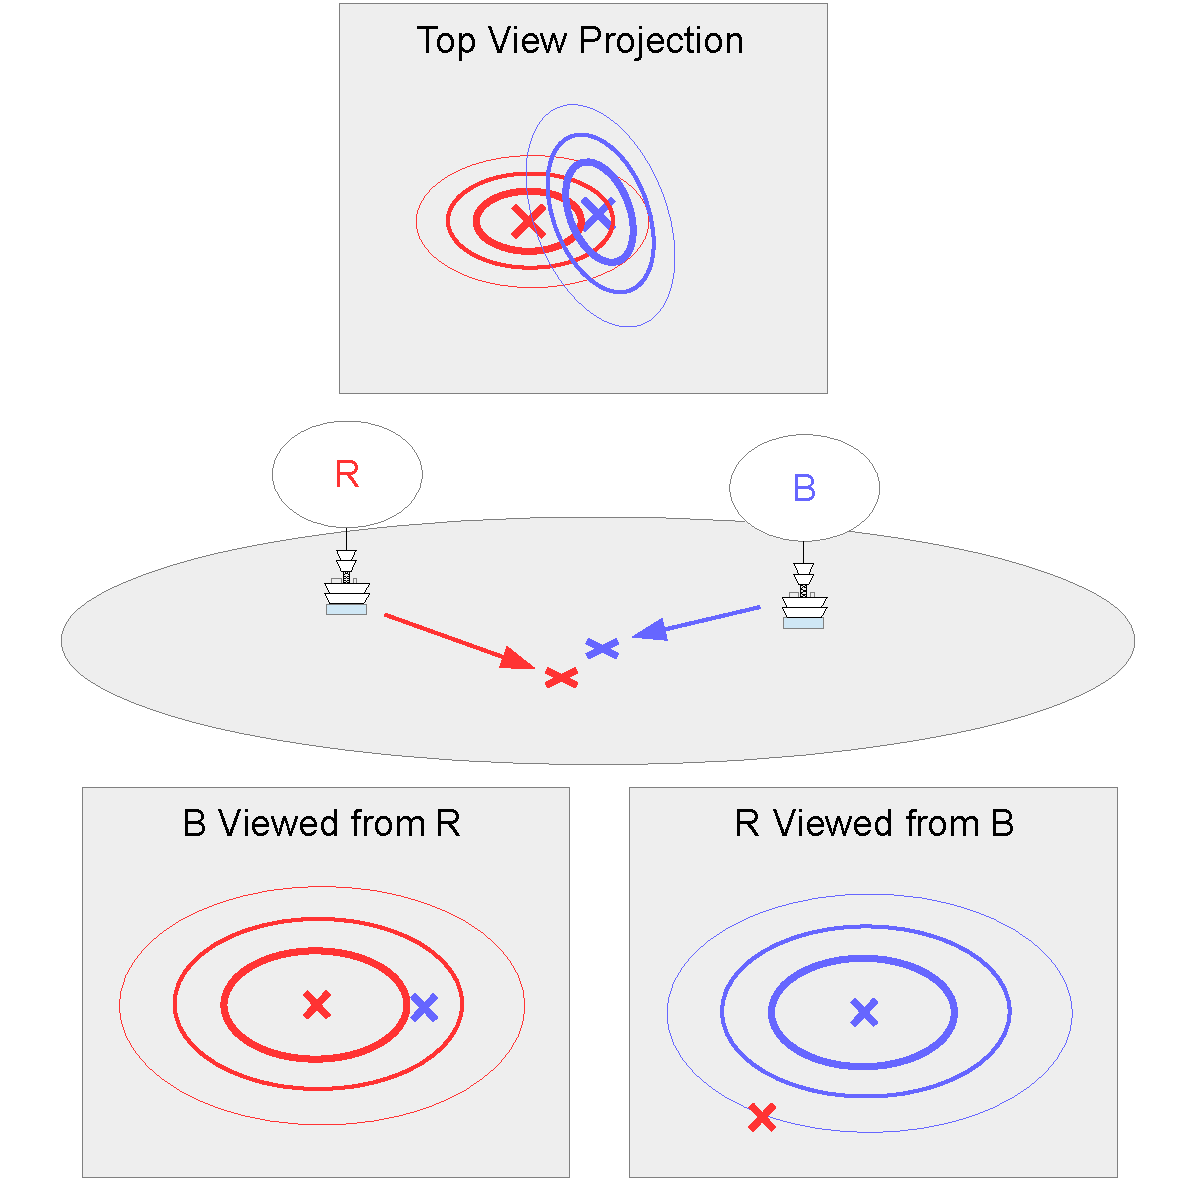
\includegraphics[width=\textwidth]{figures/clusteringProjection}
	\caption{A simplified diagram showing the projection of two events recorded from two different locations into the field of view of each other.  The Xs denote the location on the continent where the event pointed.  The elliptical paths drawn around each location represent the $1\sigma$, $2\sigma$, and $3\sigma$ pointing confidence intervals.  In this example, event B (blue) is less than$2\sigma$ away event R (red) from the point of view of event R.  However event R is more than $3\sigma$ away from event B from the perspective of event B.} 
	\label{fig:clusteringProjection}
\end{figure}
		
		
		Lets assume that we have two events that are projected nearby onto the continent, $A$ and $B$.  From the payload location where event $A$ is captured, you can measure the angular separation between the two projected positions in elevation($\theta$) and azimuth ($\phi$).  These angular separations will be denoted as $\Delta\theta_{AB}$ and $\Delta\phi_{AB}$  Equivalently, these separations can be measured from the payload position from which event $B$ was captured, which will be denoted as $\Delta\theta_{BA}$ and $\Delta\phi_{BA}$.  Since the elevation and azimuth angles are orthogonal, the total angular separation would be Equation \ref{eqn:angularSeparation}
		
	\begin{equation}
		\sqrt{\Delta\phi^2 + \Delta\theta^2}
		\label{eqn:angularSeparation}
	\end{equation}
	
	This equation however does not factor in the pointing uncertainty difference between azimuth ($\sigma_phi$) and elevation ($\sigma_theta$). Due to the longer baseline differences, elevation angles can be pointed with higher certainty than azimuthal angles.  The normalized angular separation, which has units of angular uncertainty, is shown in Equation \ref{eqn:angularSeparationNormalized}.
	
	\begin{equation}
		\sqrt{\cfrac{\Delta\phi}{\sigma_{phi}(SNR)}^2 + \cfrac{\Delta\theta}{\sigma_{theta}(SNR)}^2}
		\label{eqn:angularSeparationNormalized}
	\end{equation}
		Note that the pointing resolution  of of any single event is a function of the SNR, and thus any clustering analysis must factor this into its calculation.  The pointing resolution as a function of SNR was found from analyzing self triggered WAIS pulses and their subsequent pointing to the known calibration pulser location on the continent.  This was discussed earlier in the Calibration chapter.  Events with SNR values lower than the lowest WAIS pulse, a value of approximately 4.0, are treated as if they had the pointing uncertainty of an impulse with an SNR of 4.0.  An inverse relationship between SNR and pointing resolution is assumed based on a fit to the data.  This is shown in Equation \ref{eqn:pointVsSNR}.
		
		\begin{gather*}
		\Delta\theta = \left(\frac{A_{\theta}}{SNR}\right) + B_{\theta} \\
		\Delta\phi = \left(\frac{A_{\phi}}{SNR}\right) + B_{\phi} \\
		\label{eqn:pointVsSNR}
		\end{gather*}
				
The values determined from the fit are shown in table \ref{tab:pointVsSNRFit}.

	\begin{figure}
	\centering
	\begin{tabular}[c]{|c|c|}
	\hline
	$A_{\phi}$ & 0.68726 \\
	$B_{\phi}$ & 0.338725 \\
	$A_{\theta}$ & 0.132516 \\
	$B_{\theta}$ & 0.1557 \\
	\hline
	\end{tabular}
	\caption{Fitted parameters for inverse relationship between SNR and pointing uncertainty.  $\theta$ refers to elevation angle, and $phi$ refers to azimuth angle.}
	\label{tab:pointVsSNRFit}
	\end{figure}
	
							
		The figure of merit is then the geometric sum of the pointing uncertainty normalized angular separation from each event observation location, shown in Equation \ref{eqn:LogLikelihood}.
		
	\begin{equation}
		L = \sqrt{\frac{\Delta\phi_{AB}^2   + \Delta\phi_{BA}^2}{\sigma_{\phi}(SNR)} + \frac{\Delta\theta_{AB}^2 + \Delta\theta_{BA}^2}{\sigma_{\theta}(SNR)}}
		\label{eqn:LogLikelihood}
	\end{equation}


		Using this equation we can determine the relative ``closeness'' of any two events, as derived from the measurements and including the systematic uncertainties.
		
	
	\subsection{Distance clustering}
		Events that reconstruct with steep downward elevation angles will not have high log likelihood values even to events that occur close in physical distance.  To prevent events that may be related physically from avoiding clustering cuts, an additional condition for considering two events to be clustered is that they fall within 50km of each other on the ice.  This is calculated using the great circle distance between the mapped locations of the events onto the ice.
	
	\subsection{Impulsive source identification}
		In order to exclude events that are likely to be anthropogenic background, it is necessary to determine locations on the continent from which impulsive RF transients are produced.  Since events created by Humans are likely to emanate from discrete sources, this can be done by determining locations in which many impulsive events occur close to one another.  This is done by marking events that fall within a log likelihood of $L<40$ from any other event.  Events with a single other event falling within this threshold are marked as pseudo-bases.  By keeping the information for all events that fall within a cluster, instead of combining them to a single mean point, clustered impulsive source locations become elongated and exclude a larger region of the instrumental exposure.  This is done conservatively to keep anthropogenic background from leaking into the signal region.
		
	\subsection{Event Clustering}
		The final set of signal cuts will provide a set of events that are most likely to be signal.  These events are then clustered with all events tagged as pseudo-bases, and removed from the signal sample if they do.  The remaining events will then be isolated impulsive transients that closely match the simulated radiation from an EAS, and will be the final candidates of the analysis.



	